\section{Results}

\subsection{Description of the stroke and matched control populations}

There were 236,630 instances in each of the matched populations (stroke and control populations). Table \ref{tab:populations} shows the descriptive statistics of the main features.

\begin{table}[!ht]
    \centering
    \begin{tabular}{|l|l|l|l|}
    \hline
        \multicolumn{2}{|c|}{\bf Population cohort} & \bf Stroke & \bf Control \\ \hline
        \multicolumn{2}{|l|}{\bf Matched populations} & 236,630 & 236,630 \\ \hline
        \multirow{2}{*}{\bf Sex} & \bf Female & 110595 & 110595 \\
        & \bf Male & 126,035 & 126,035 \\ \hline
        \multirow{5}{*}{\bf Age, years} & \bf 0-20 & 130 & 240 \\
        & \bf 20-40 & 4460 & 5660 \\
        & \bf 40-60 & 36,915 & 42,565 \\
        & \bf 60-80 & 109,170 & 116,220 \\
        & \bf 80+ & 85,950 & 71,945 \\
        & \bf Mean [std] & 74 [13.7] & 71 [13.8] \\ \hline
        \multirow{5}{*}{\bf IMD quintiles (2019)} & \bf 1 & 48050 & 36155 \\
        & \bf 2 & 46,820 & 43,155 \\
        & \bf 3 & 48,305 & 49,680 \\
        & \bf 4 & 48,210 & 53,355 \\
        & \bf 5 & 45,250 & 54,285 \\ \hline
        \multirow{5}{*}{\bf Ethnicity} & \bf White & 213,240 & 213,240 \\
        & \bf Asian or Asian British & 12,160 & 12,160 \\
        & \bf Black, Black British, Caribbean or African & 6,545 & 6,545 \\
        & \bf Other ethnic group & 2,085 & 2,085 \\
        & \bf Mixed or multiple ethnic groups & 1,645 & 1,645 \\
        & \bf Unknown & 955 & 955 \\ \hline
        \multirow{4}{*}{\bf Covid} & \bf Infection only & 3,445 & 415 \\
        & \bf Vaccination only & 124,965 & 128,500 \\
        & \bf Vaccination and infection & 5,105 & 1,210 \\
        & \bf None & 103,115 & 106,510 \\ \hline
        \multirow{9}{*}{\bf Region} & \bf South East & 35,680 & 41,125 \\
        & \bf North West & 35,295 & 30,705 \\
        & \bf South West & 29,145 & 27,435 \\
        & \bf East of England & 26,160 & 27,965 \\
        & \bf Yorkshire and The Humber & 24,880 & 23,055 \\
        & \bf West Midlands & 24,275 & 25,085 \\
        & \bf London & 24,055 & 28,605 \\
        & \bf East Midlands & 22,390 & 21,120 \\
        & \bf North East & 14,750 & 11,535 \\ \hline
        \multirow{2}{*}{\bf Rural/urban (2011)} & \bf Urban & 188,895 & 185,025 \\
        & \bf Rural & 47,740 & 51,605 \\ \hline
    \end{tabular}
    \caption{Descriptive statistics of the main features for the 236,630 instances in the matched stroke and control populations. Counts to the nearest 5. Age of stroke patients was as recorded in SSNAP, while age of control patients was as recorded in demographic data (matching was performed using ages in demographic data)}.
    \label{tab:populations}
\end{table}

In the year following a stroke, stroke patients spent, on average (mean), 266.4 days at home (sd 138.6), 23.2 days in care (sd 32.7) and 75.5 days dead (sd 135.7). This was in comparison to the matched control population spending, on average (mean), 352.8 days at home (sd 50.8), 2.4 days in care (sd 10.2) and 9.8 days dead (sd 48.0). When comparing individual matched patients, stroke patients spent, on average (mean), 86.4 days less at home (sd 143.5), 20.8 more days in care (sd 34.1), and died 65.7 days sooner (sd 140.5). Detailed results for the stroke and control matched population are given in the supplementary material.

%%%%%%%%%%%%%%%%%%%%%%%%%%%%%%%%%%%%%%%%%%%%%%%%%%%%%%%%%%%%%%%%%%%%%%%
\subsection{Survival analysis following stroke}

Survival analysis was performed on the full stroke population.

We defined the baseline characteristics of a patient to be: white; under 60 years old; living in the 20\% most deprived area; had no Covid vaccination within 12 months of stroke event; had no Covid infection within 30 days of stroke event; receive no acute treatment (thrombolysis or thrombectomy), no diabetes, no arterial fibrillation, precisely known onset time, infarction, onset out of hospital and arrive within 6 hours. The survival rate of the baseline stroke patient for the exploratory population and the causal population in the first year following a stroke event is shown in figure \ref{survival_baseline}. Within 50 days of their stroke 10.5\% of the full exploratory stroke population have died, and 22.0\% being dead by the end of the first year following their stroke. In comparison, 9.3\% of the causal stroke population have died within the first year of the stroke event, and 19.9\% being dead at the end of the first year following their stroke.

The effect of a patients characteristics deviating from this defined baseline stroke patient (for each population: exploratory and causal) are shown as hazard ratios for each feature as a forest plot (figure \ref{fig:forest_plot_main}) with the features ranked by impact on survival.

\begin{figure}[ht]
  \centering
  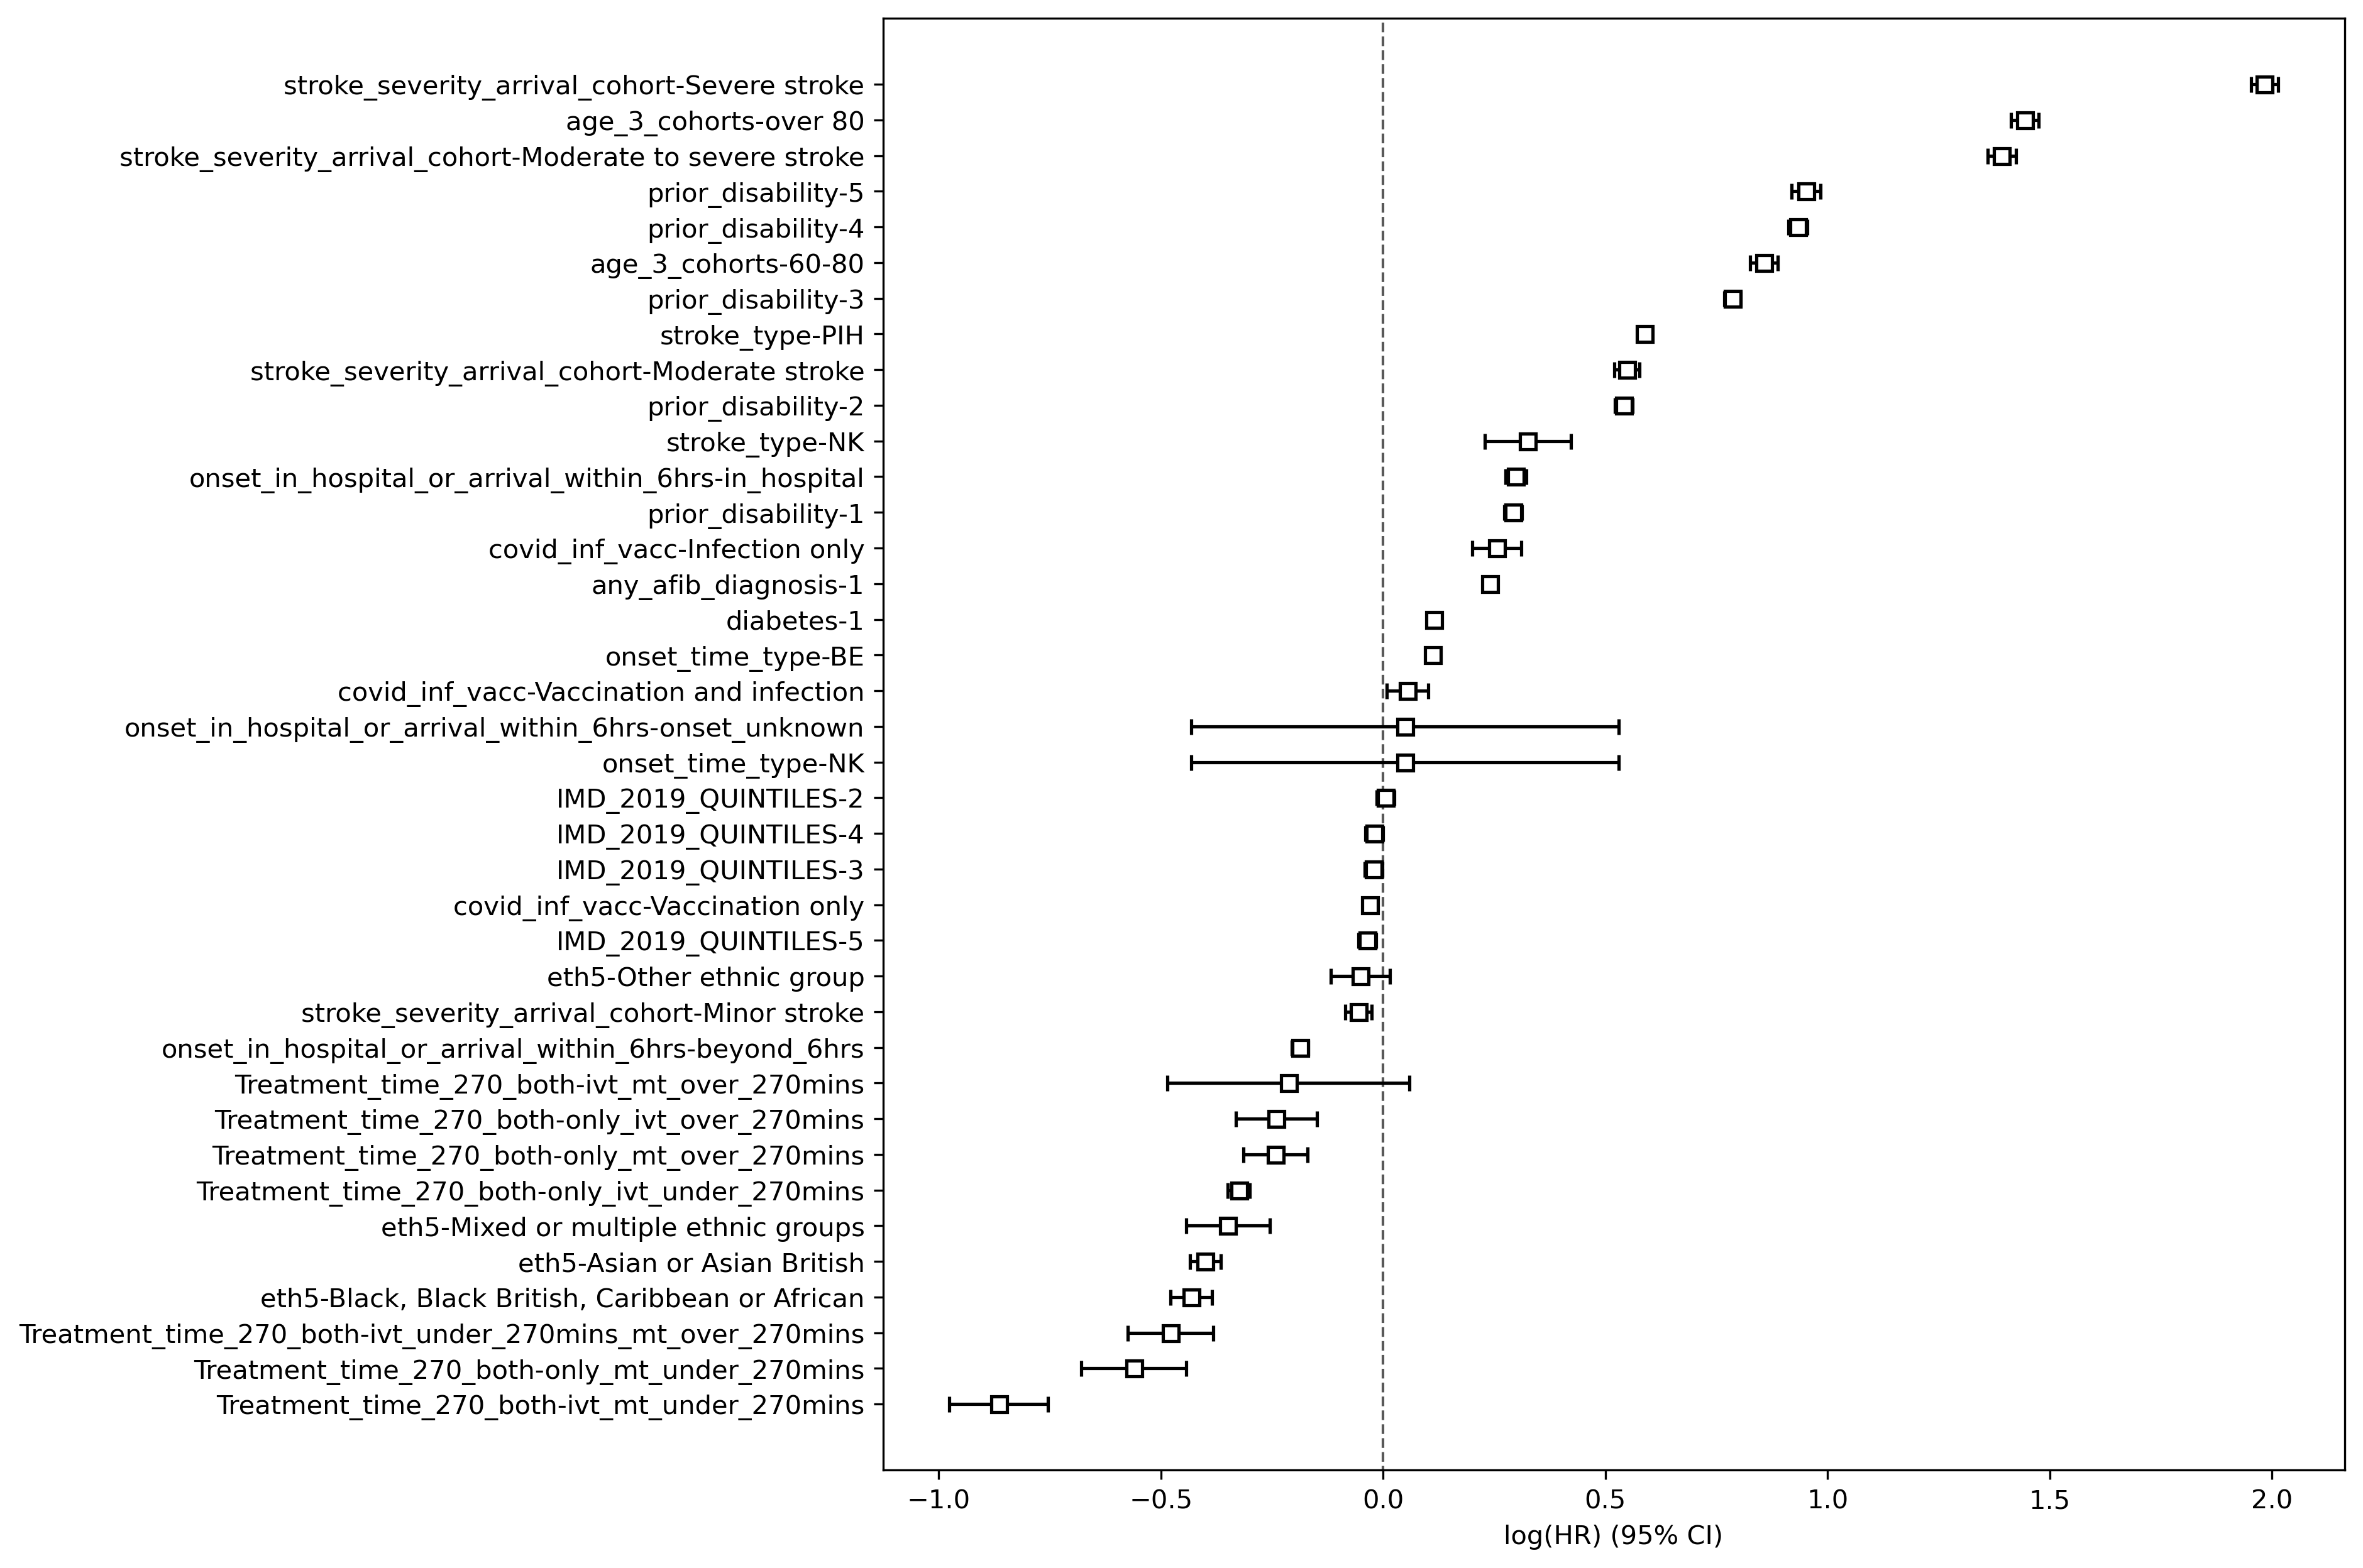
\includegraphics[width=1.0\textwidth]{./images/output_results_from_SDE/ccu085_040_forest_plot_hazard_ratios_from_cox_proportional_hazard_ratio_model_survival_in_year_following_stroke_exploratory_population}
  \caption{Forest plot of one-year post-stroke survival rates, with reference (baseline) categories defined as: white ethnicity; age under 60 years; residence in the most deprived 20\% of areas; no Covid-19 vaccination within 12 months before stroke; no Covid-19 infection within 30 days before stroke; no acute treatment received (thrombolysis or thrombectomy); no stroke symptoms present on arrival; no pre-existing disability; no diabetes; no atrial fibrillation; ischaemic stroke subtype; community (out-of-hospital) onset; and arrival within 6 hours of onset.}
  \label{fig:forest_plot_main}
\end{figure}

The five characteristics (deviating from the baseline characteristics) that had the largest impact on increasing the risk of death of a stroke patient in the first year following their stroke were: 1. having a severe stroke (rather than no stroke symptoms); 2. being over 80 years old (rather than under 60); 3. having a moderate to severe stroke (rather than no stroke symptoms); 4. having a prior disability of mRS5 (rather than mRS0); 5. having a prior disability of mRS4 (rather than mRS0). These characteristics increased risk of death by 727\%, 424\%, 402\%, 259\%, and 254\%. 

The five characteristics (deviating from the baseline characteristics) that had the largest impact on reducing the risk of death of a stroke patient (from the exploratory population) in the first year following their stroke are: 1. having early IVT and MT (rather than no treatment); 2. early MT only (rather than no treatment; 3. early IVT with late MT (rather than no treatment; 4. Black (rather than white); 5. Asian (rather than white). These characteristics reduced a patients risk of death by 42\%, 57\%, 62\%, 65\%, and 67\%.

%%%%%%%%%%%%%%%%%%%%%%%%%%%%%%%%%%%%%%%%%%%%%%%%%%%%%%%%%%%%%%%%%%%%%%%

\subsection{Explainable machine learning}

When investigating the full stroke population, twelve features were chosen to investigate how patient characteristics affect outcomes (see Supplementary Material for detailed results). With these features selected, the R-squared for prediction of time spent in care, at home, or dead, were  12.0\% 38.0\ and 34.7\%. 

Figures \ref{fig:shap_1} to \ref{fig:shap_3} show how general patient characteristics affect model predictions. General observations are, common across both models, unless otherwise commented on:

\begin{itemize}
    \item \textit{Stroke severity}: Time in NHS inpatient care increased and then reduced with increasing stroke severity. Time at home reduced with increasing stroke severity, while time dead increased.

    \item \textit{Prior disability}: Time in NHS inpatient care increased and then reduced with increasing prior disability. Time at home reduced with increasing prior disability, while time dead increased.

    \item \textit{Age}: There was no clear pattern in time in NHS inpatient care with age, but time at home reduced with increasing age, while time dead reduced.

    \item \textit{Ethnicity}: Being in Black, Mixed, and Other ethnic groups led to a prediction of higher time in NHS inpatient care. Being in White ethnic group, compared to other groups, led to lower predictions of time at home, and higher predictions of time dead.

    \item \textit{Deprivation} (IMD quintile): Increasing deprivation predicted slightly higher time in care, slightly lower time at home, slightly higher time dead.

     \item \textit{Covid status}: Covid infection, with or without vaccine led to a prediction of higher length in NHS inpatient care. Covid infection without vaccine led to predictions of lower time and at home, and more time dead. The effect of Covid infection was largely ameliorated by having being vaccinated.

     \item \textit{Stroke type}: Stroke type did not significantly alter predictions of time in care, but hemorrhagic stroke (adjusting for stroke severity) was associated with less time at home, and more time dead, compared to ischemic stroke.

     \item \textit{Atrial fibrillation}: A diagnosis of atrial fibrillation made little difference to predicted time in NHS inpatient care, but led to lower predicted time at home, and higher predicted time dead.

     \item \textit{Diabetes}: A diagnosis of diabetes led to a prediction of a little more time in care, less time at home and more time dead.    
\end{itemize}

Examining how reperfusion treatment received affects predicted outcomes was performed using the full stroke population which all used predictive features, and in a population and choice of features chosen to better isolate the causal influence of treatment (figure \ref{fig:shap_4}).

Across both models were the observations, after adjusting for all other features in the models were:

\begin{itemize}
    \item Early treatment with IVT and MT predicted lower time in NHS inpatient care, more time at home, and less time dead.

    \item Early treatment with IVT but late treatment with MT predicted increased time in NHS inpatient care, but less at home. The models differ in whether time dead is increased or reduced.

    \item Early treatment with IVT alone was associated with slightly lower time in NHS inpatient care, and more time at home (with little difference time dead).

     \item Early treatment with MT alone was associated with little difference in time in care, time at home, or time at home outcomes.

     \item Late treatment with both IVT and MT was associated with less time at home or more time dead. The models differ in whether time in NHS inpatient care was increased or largely unchanged.

     \item Late treatment with IVT alone predicted little change in outcome.

     \item Late treatment with MT alone predicted longer length of stay in NHS inpatient care, less time at home, and more time dead.     
    
\end{itemize}

%%%%%%%%%%%%%%%%%%%%%%%%%%%%%%%%%%%%%%%%%%%%%%%%%%%%%%%%%%%%%%%%%%%%%%%%

\begin{figure}[htbp]
    \centering

    % ---------- Row 1 ----------
    
    \begin{subfigure}[t]{0.31\textwidth}
        \centering
        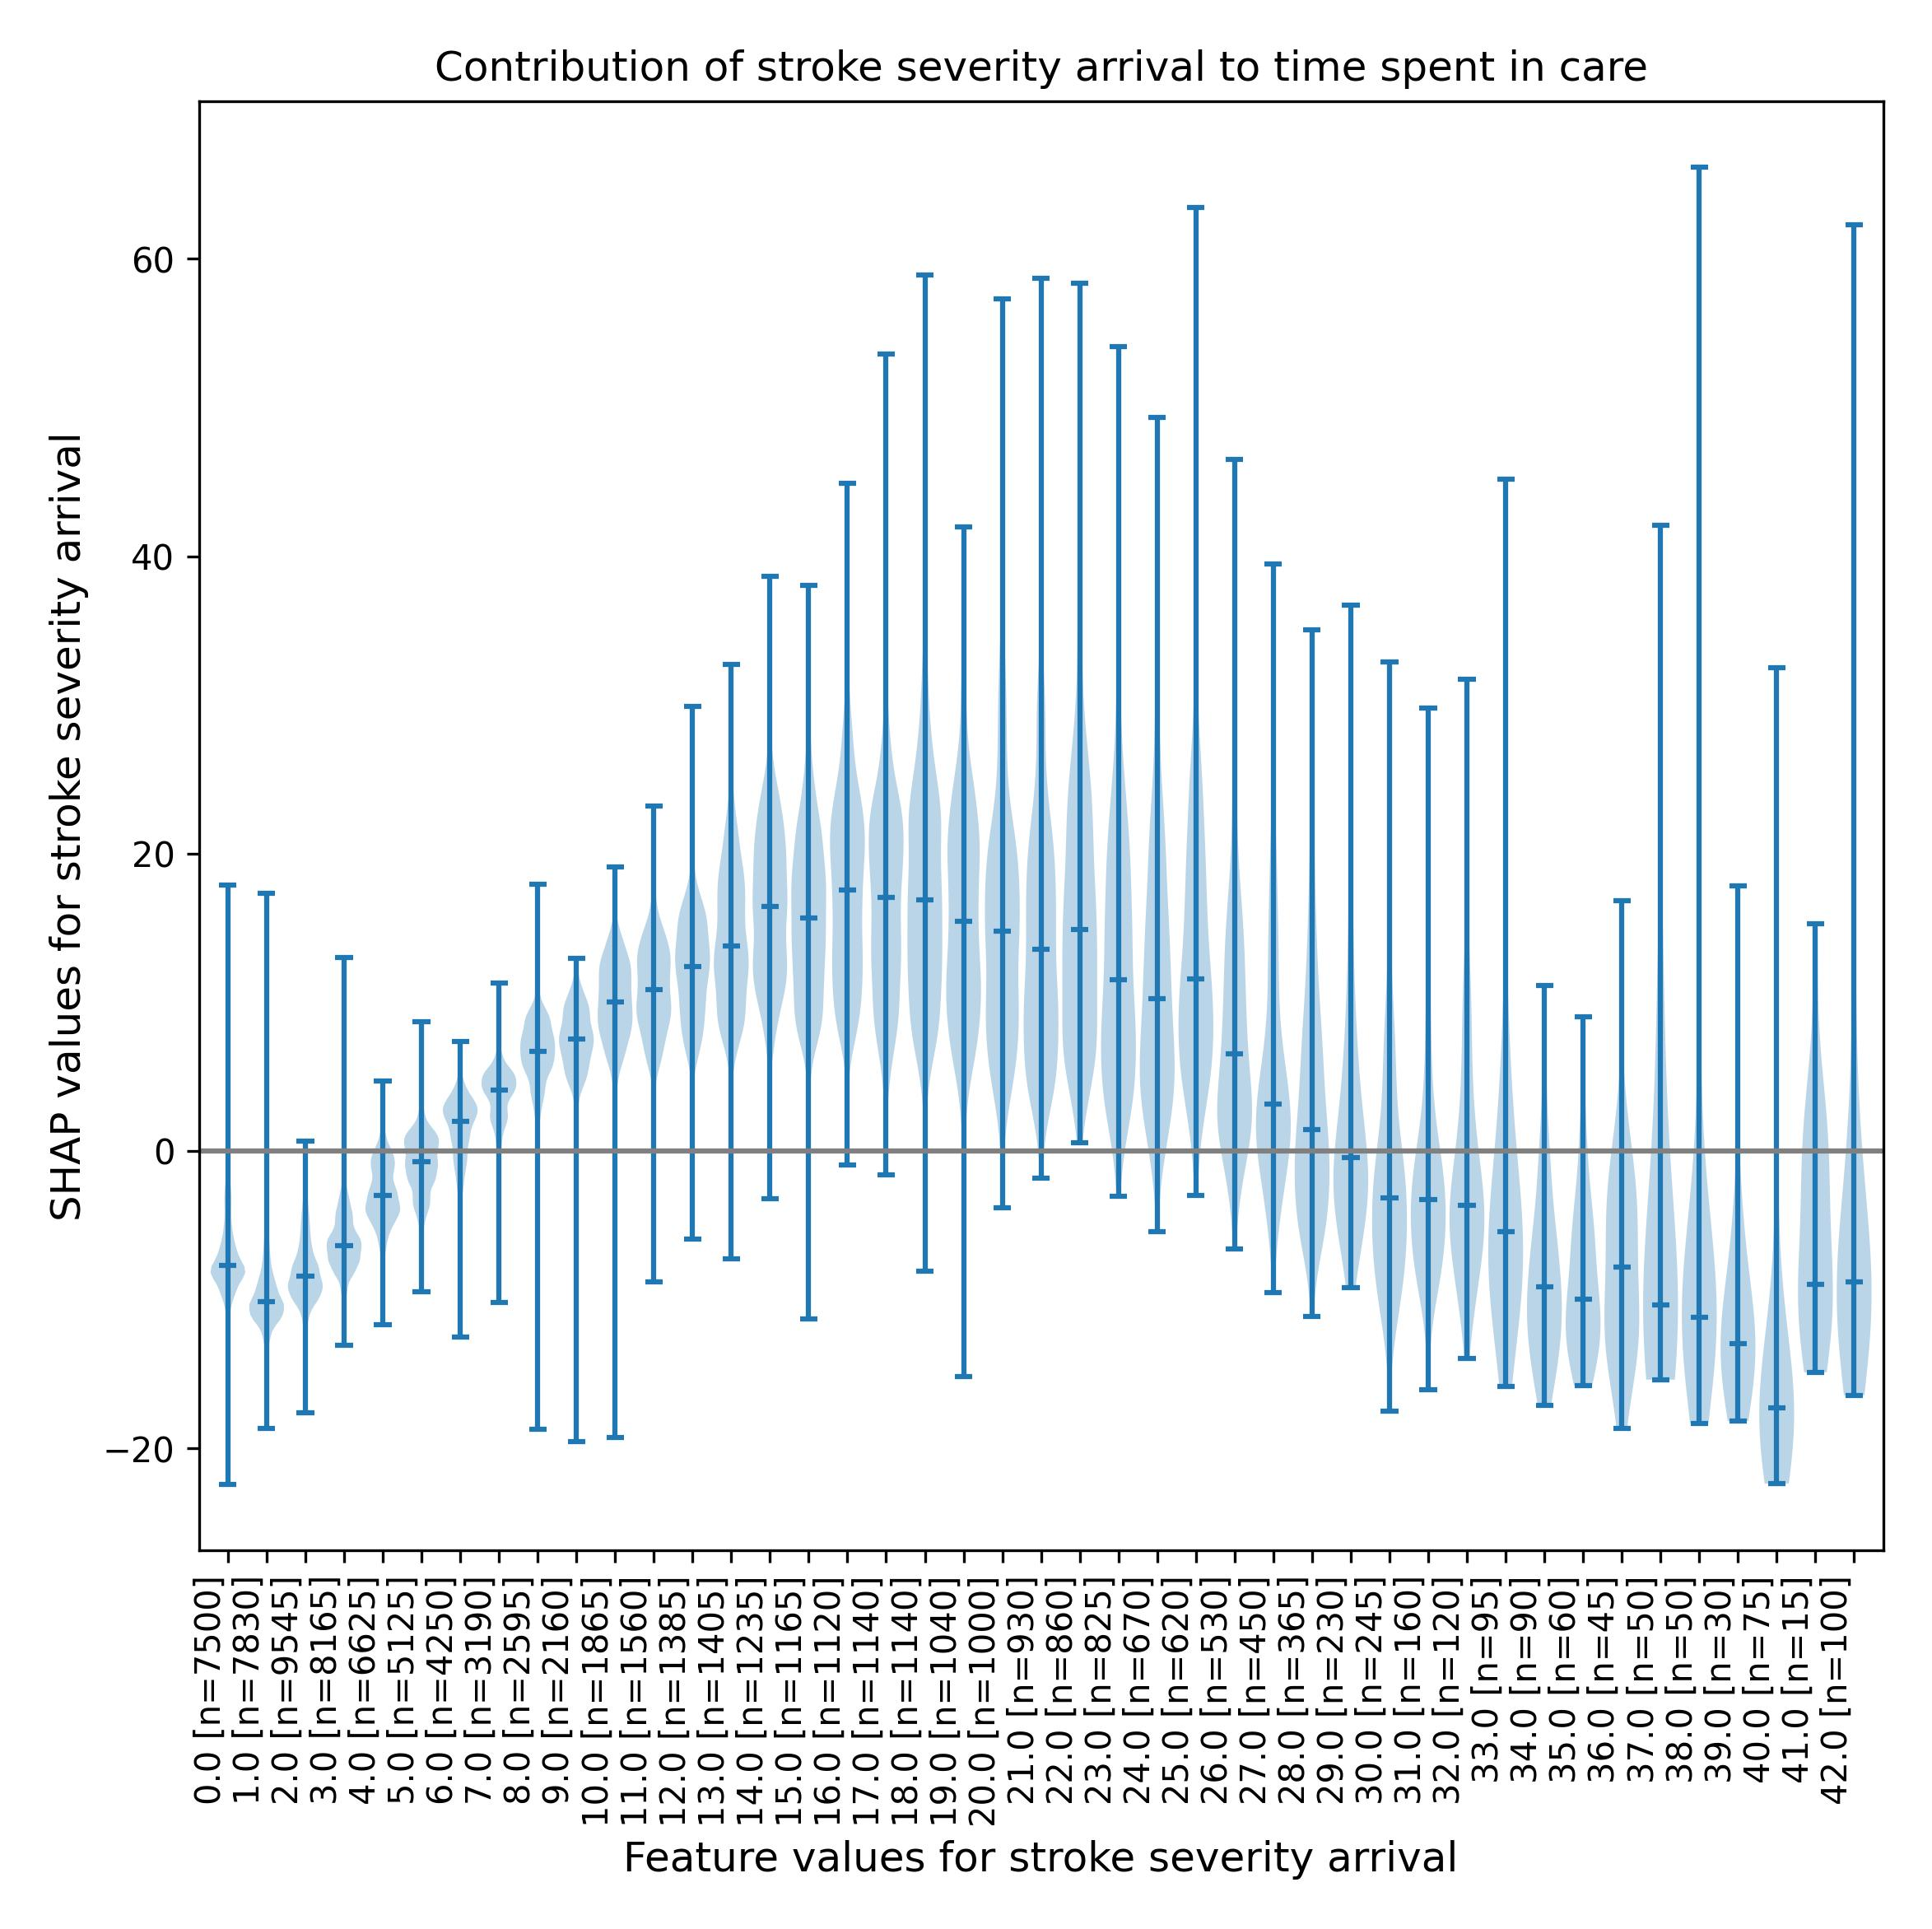
\includegraphics[width=\linewidth]{images/output_results_from_SDE/180_xgboost_in_care_exploratory_population_12_features_violin_shap_stroke_severity_arrival_kfold0.jpg}
        \caption{In care}
        \label{fig:sub1}
    \end{subfigure}
    \hfill
    \begin{subfigure}[t]{0.31\textwidth}
        \centering
        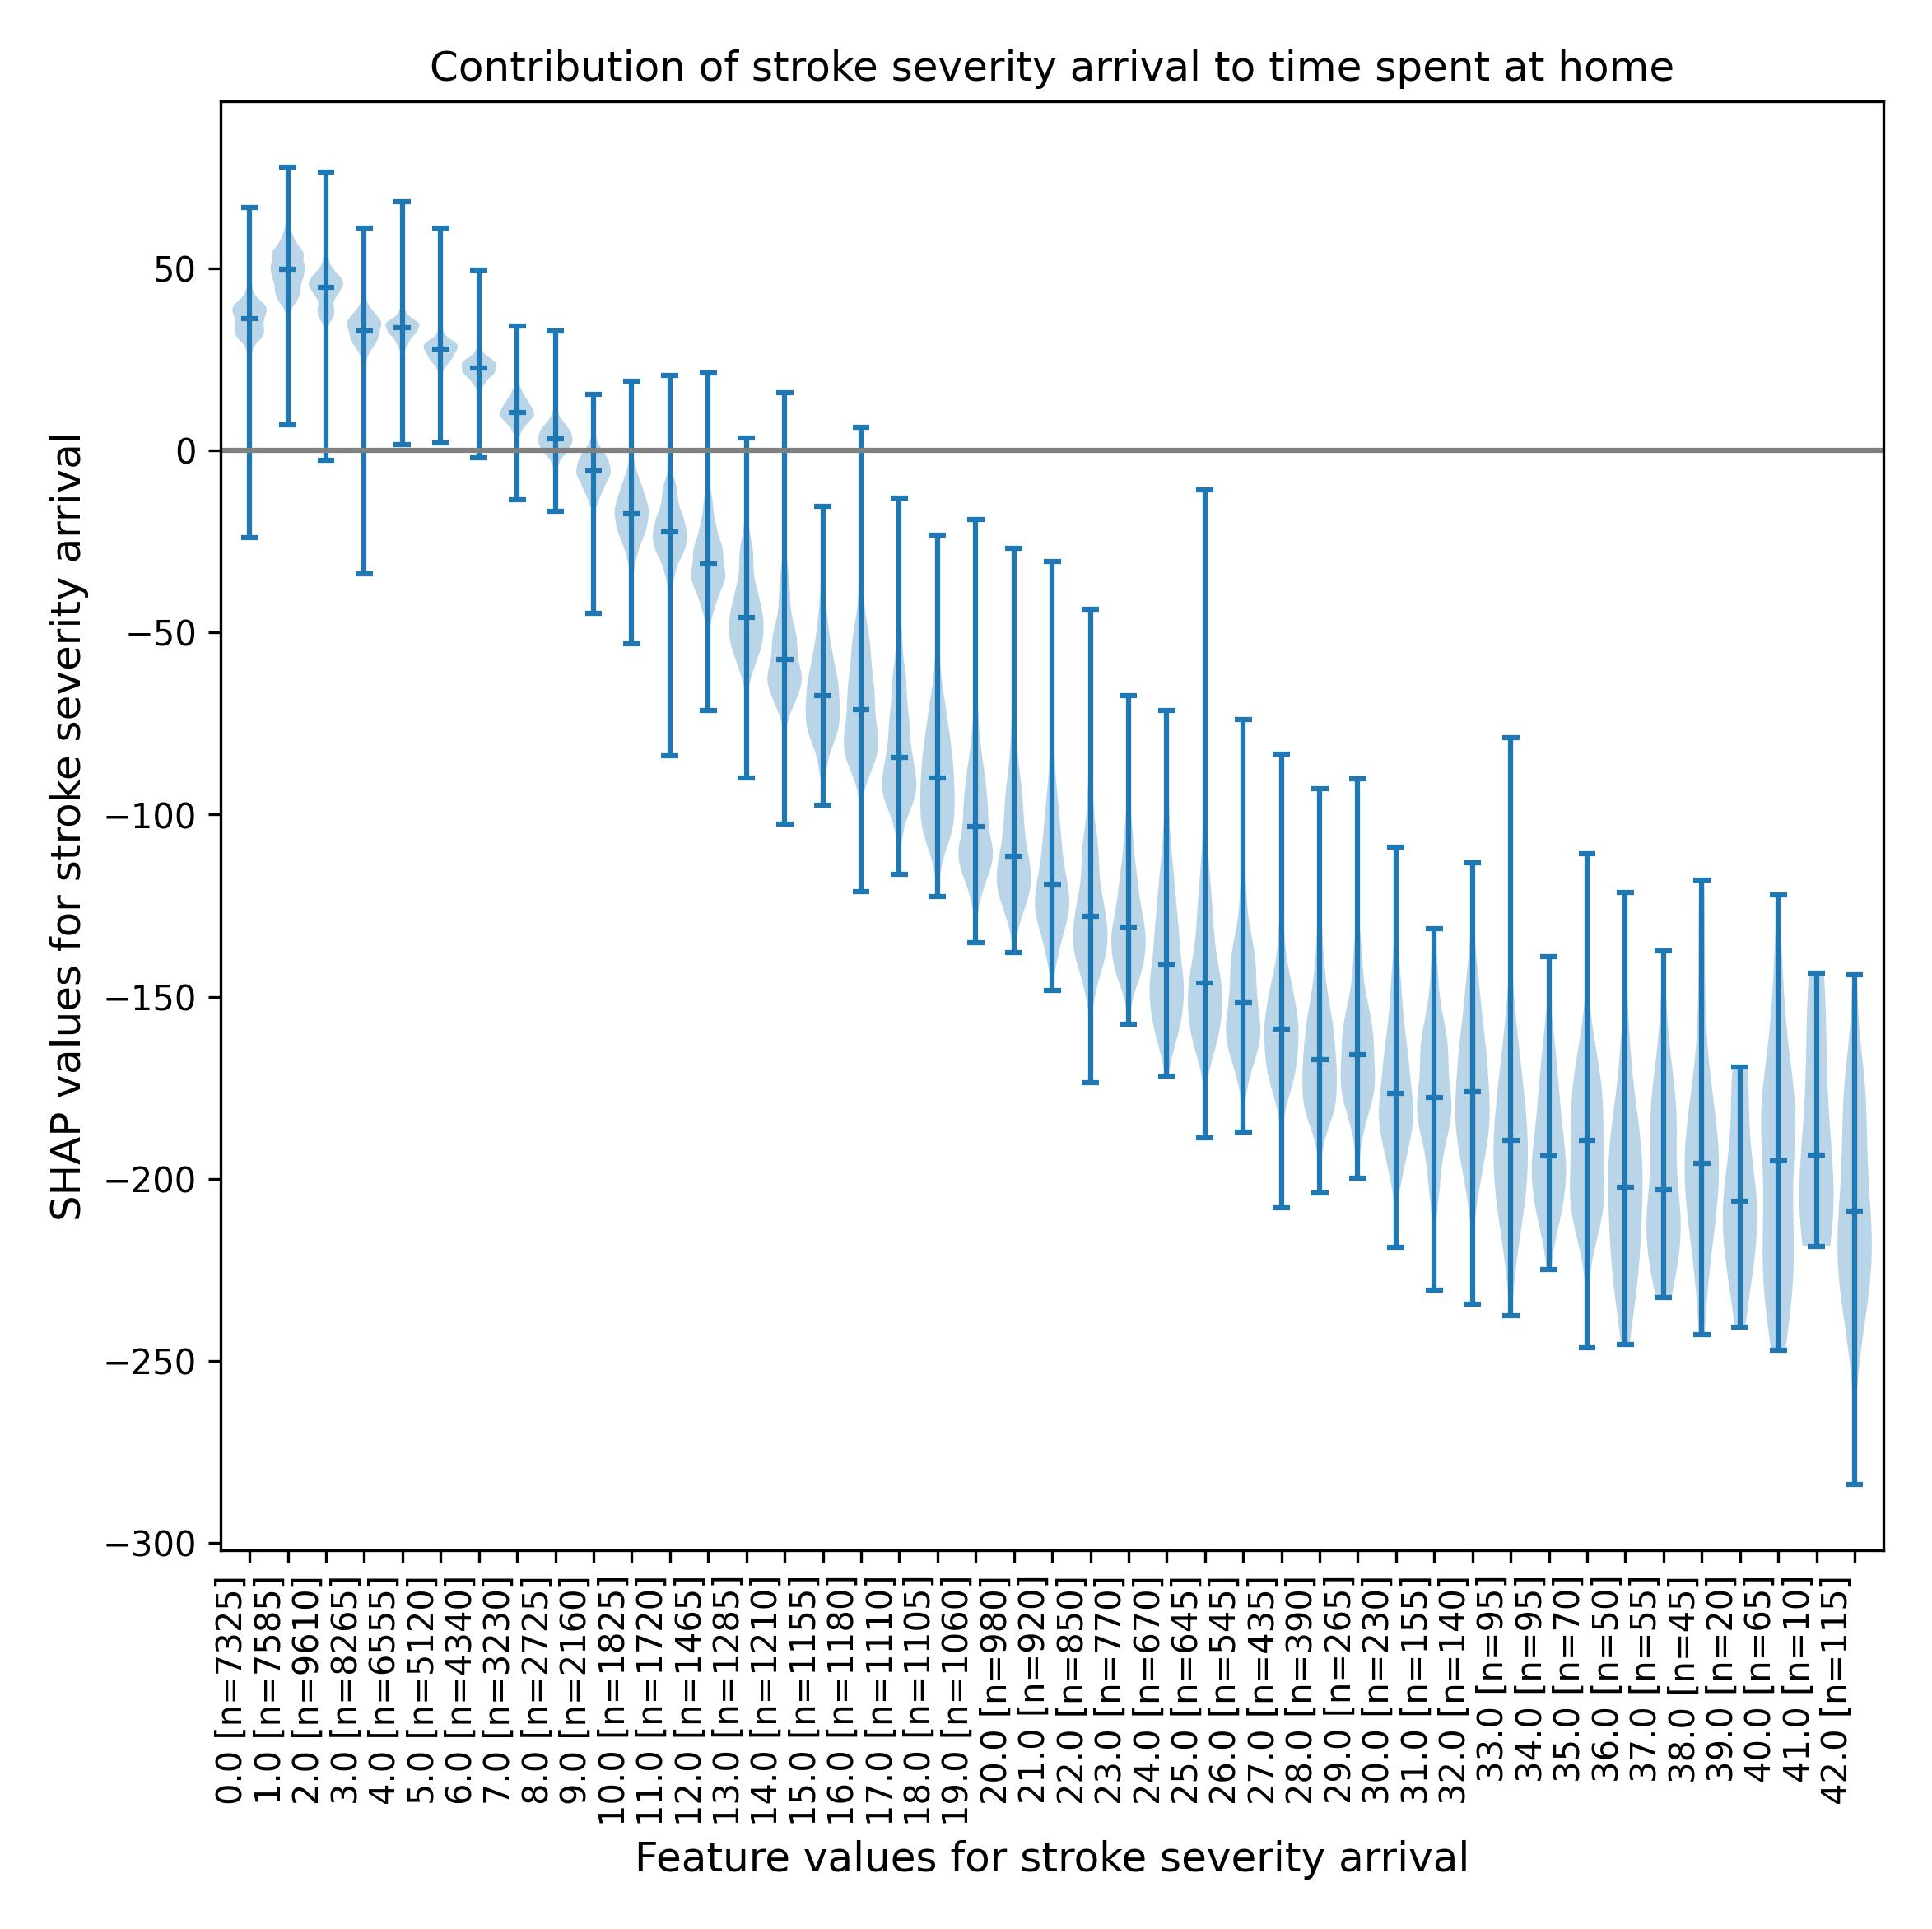
\includegraphics[width=\linewidth]{images/output_results_from_SDE/190_xgboost_at_home_exploratory_population_12_features_violin_shap_stroke_severity_arrival_kfold0.jpg}
        \caption{At home}
        \label{fig:sub2}
    \end{subfigure}
    \hfill
    \begin{subfigure}[t]{0.31\textwidth}
        \centering
        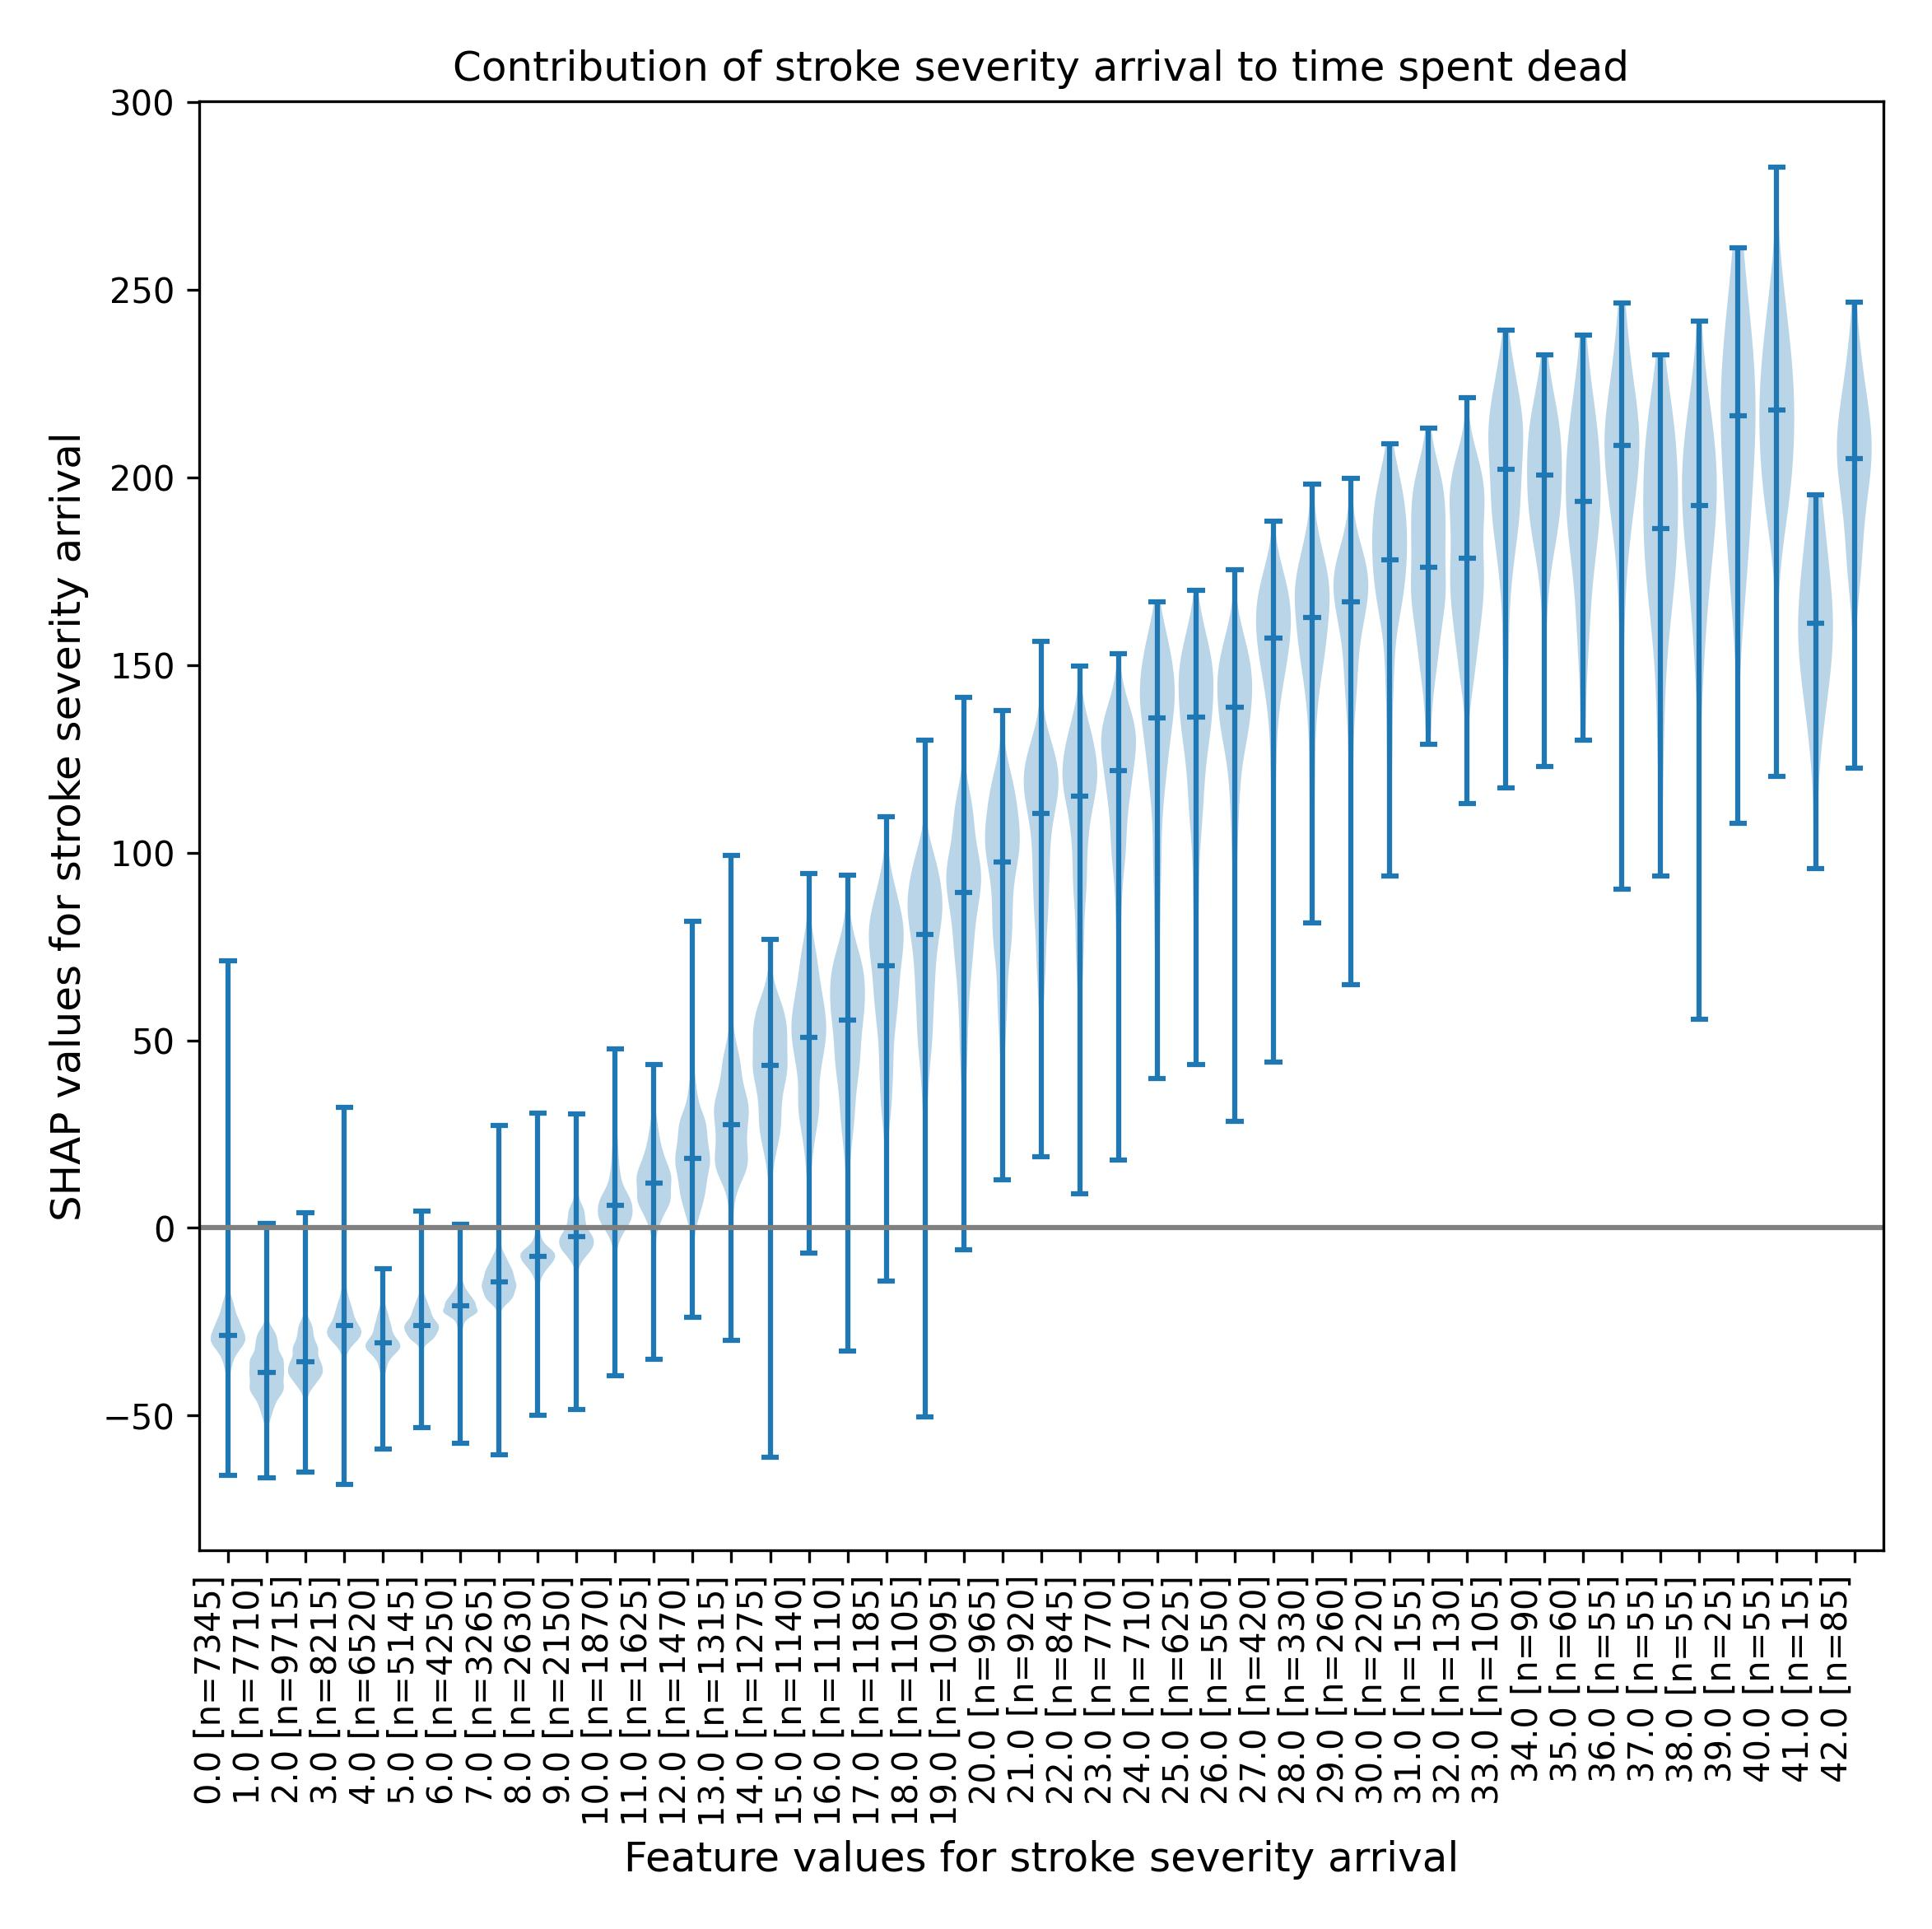
\includegraphics[width=\linewidth]{images/output_results_from_SDE/200_xgboost_dead_exploratory_population_12_features_violin_shap_stroke_severity_arrival_kfold0.jpg}
        \caption{Dead}
        \label{fig:sub3}
    \end{subfigure}
    \caption*{Stroke severity}

    \vspace{2em} % space between rows

    % ---------- Row 2 ----------
    \begin{subfigure}[t]{0.31\textwidth}
        \centering
        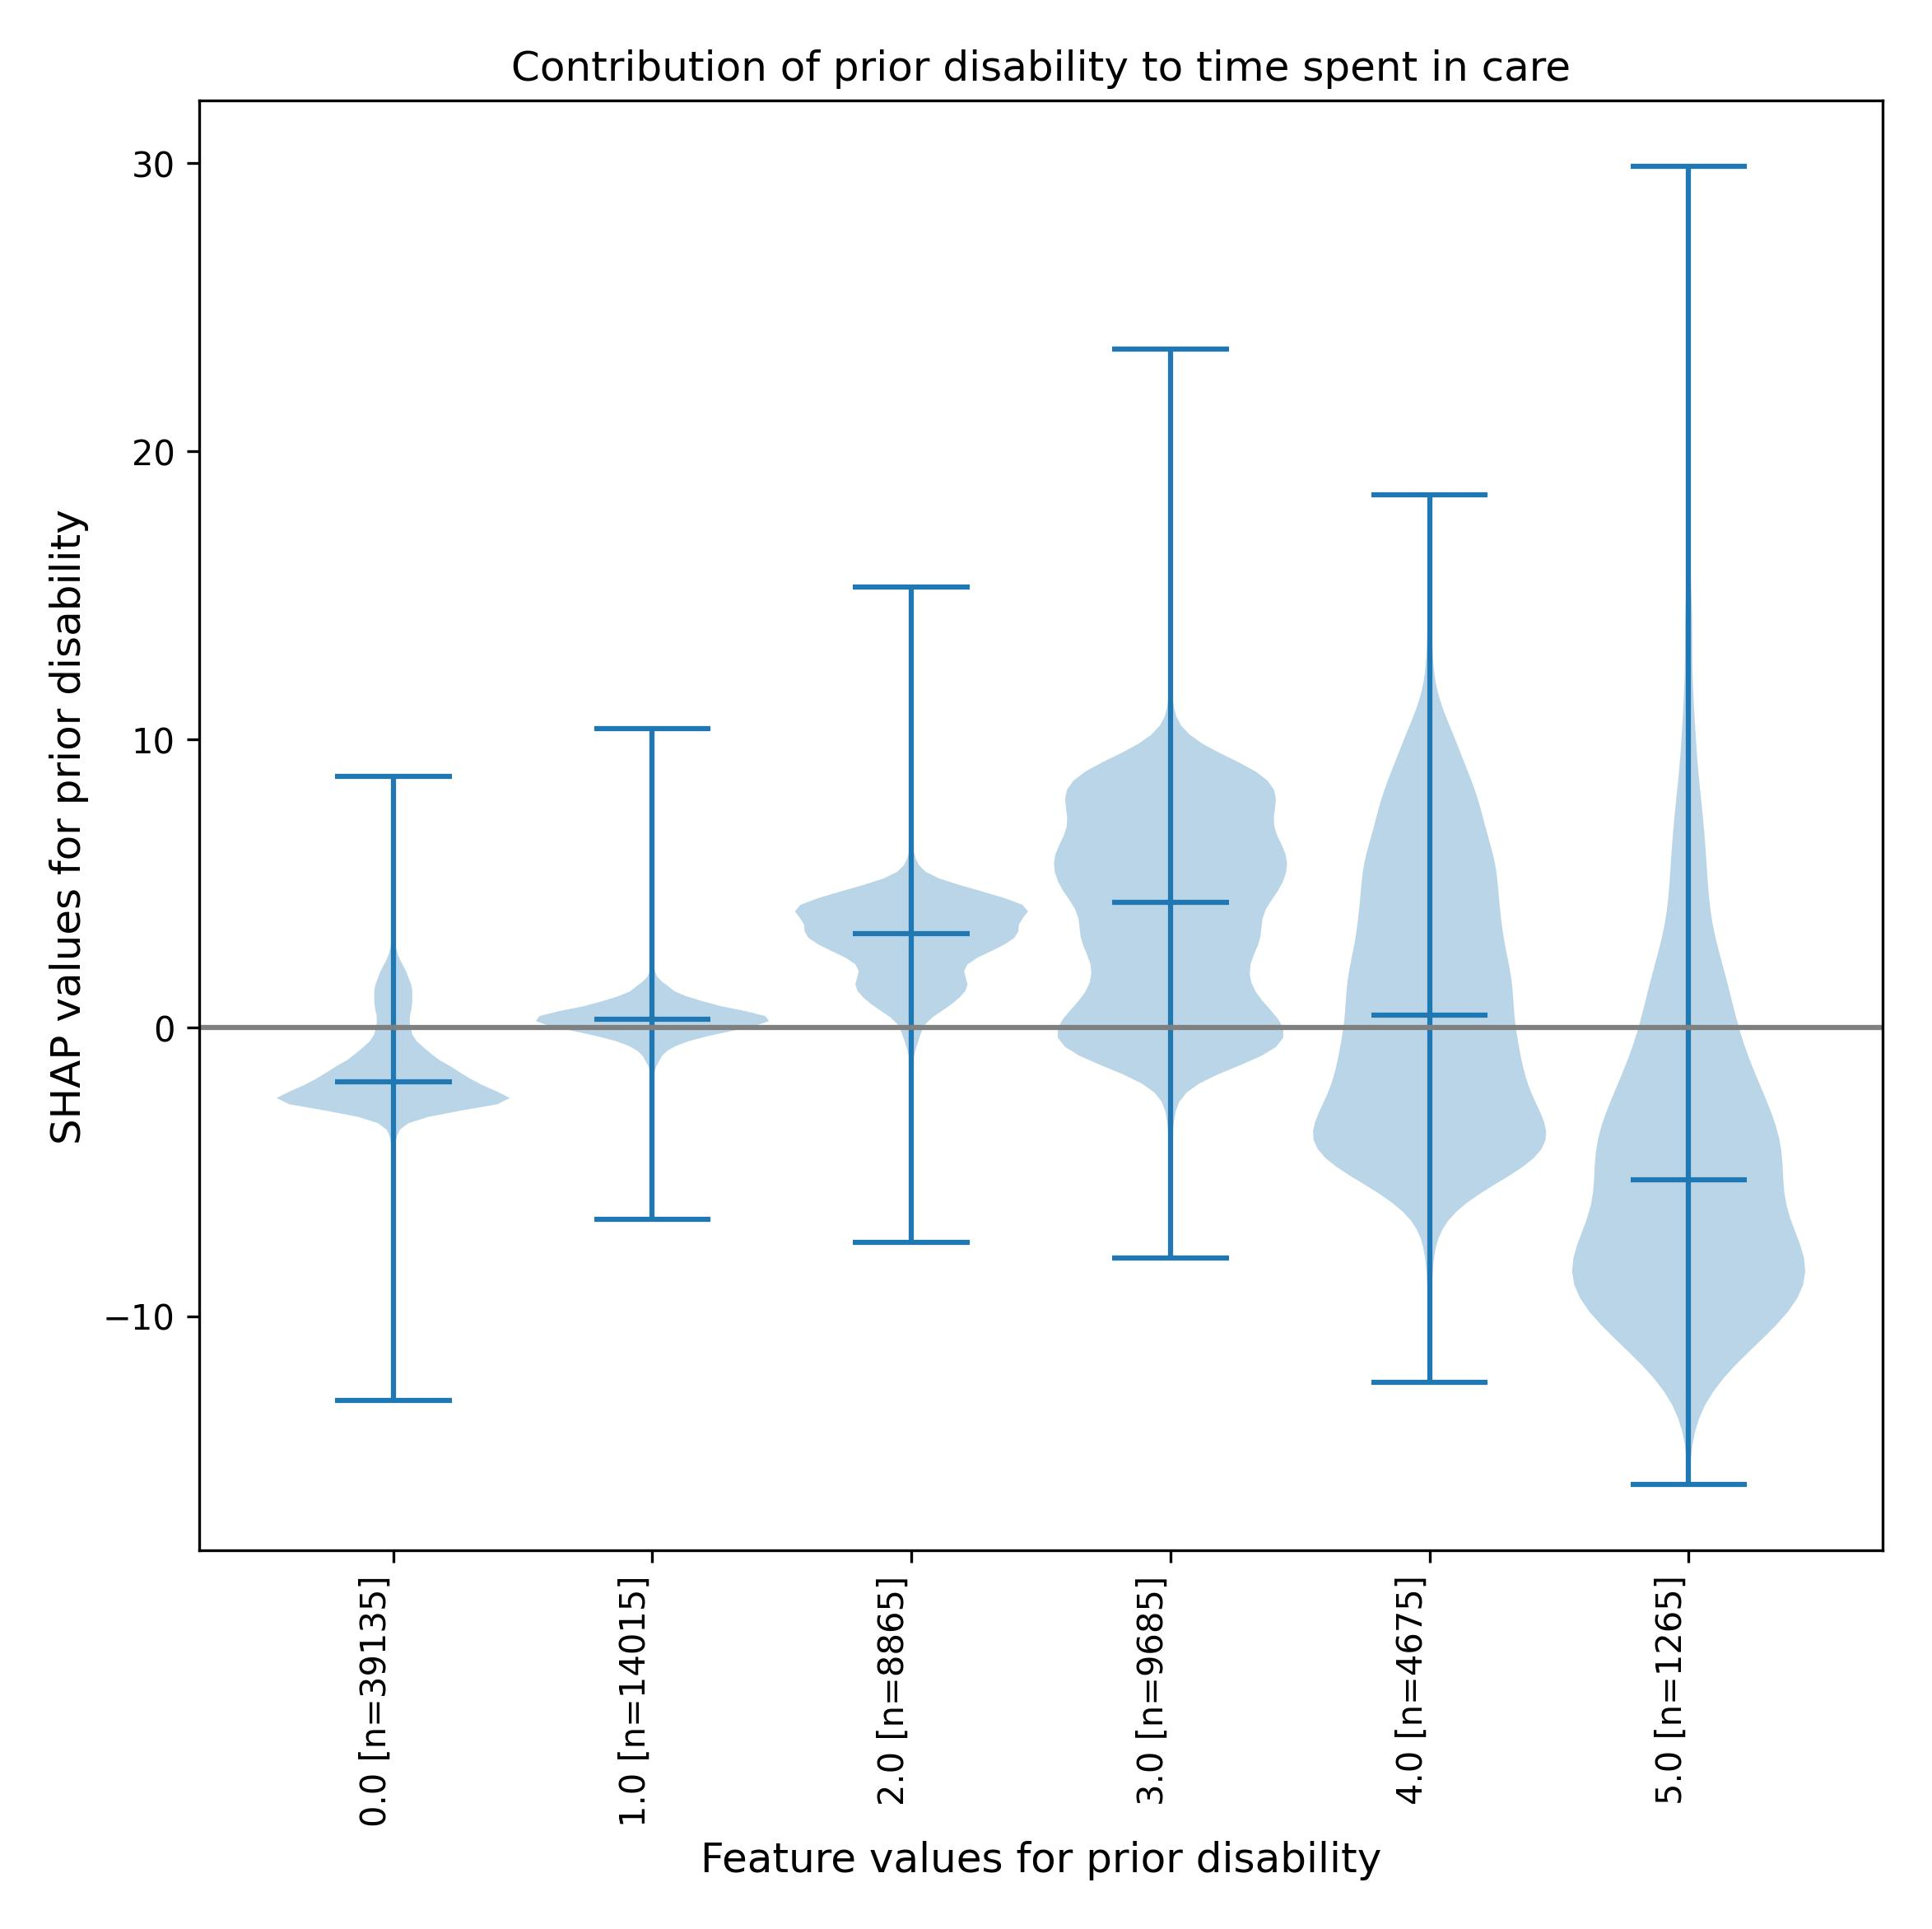
\includegraphics[width=\linewidth]{images/output_results_from_SDE/180_xgboost_in_care_exploratory_population_12_features_violin_shap_prior_disability_kfold0.jpg}
        \caption{In care}
        \label{fig:sub4}
    \end{subfigure}
    \hfill
    \begin{subfigure}[t]{0.31\textwidth}
        \centering
        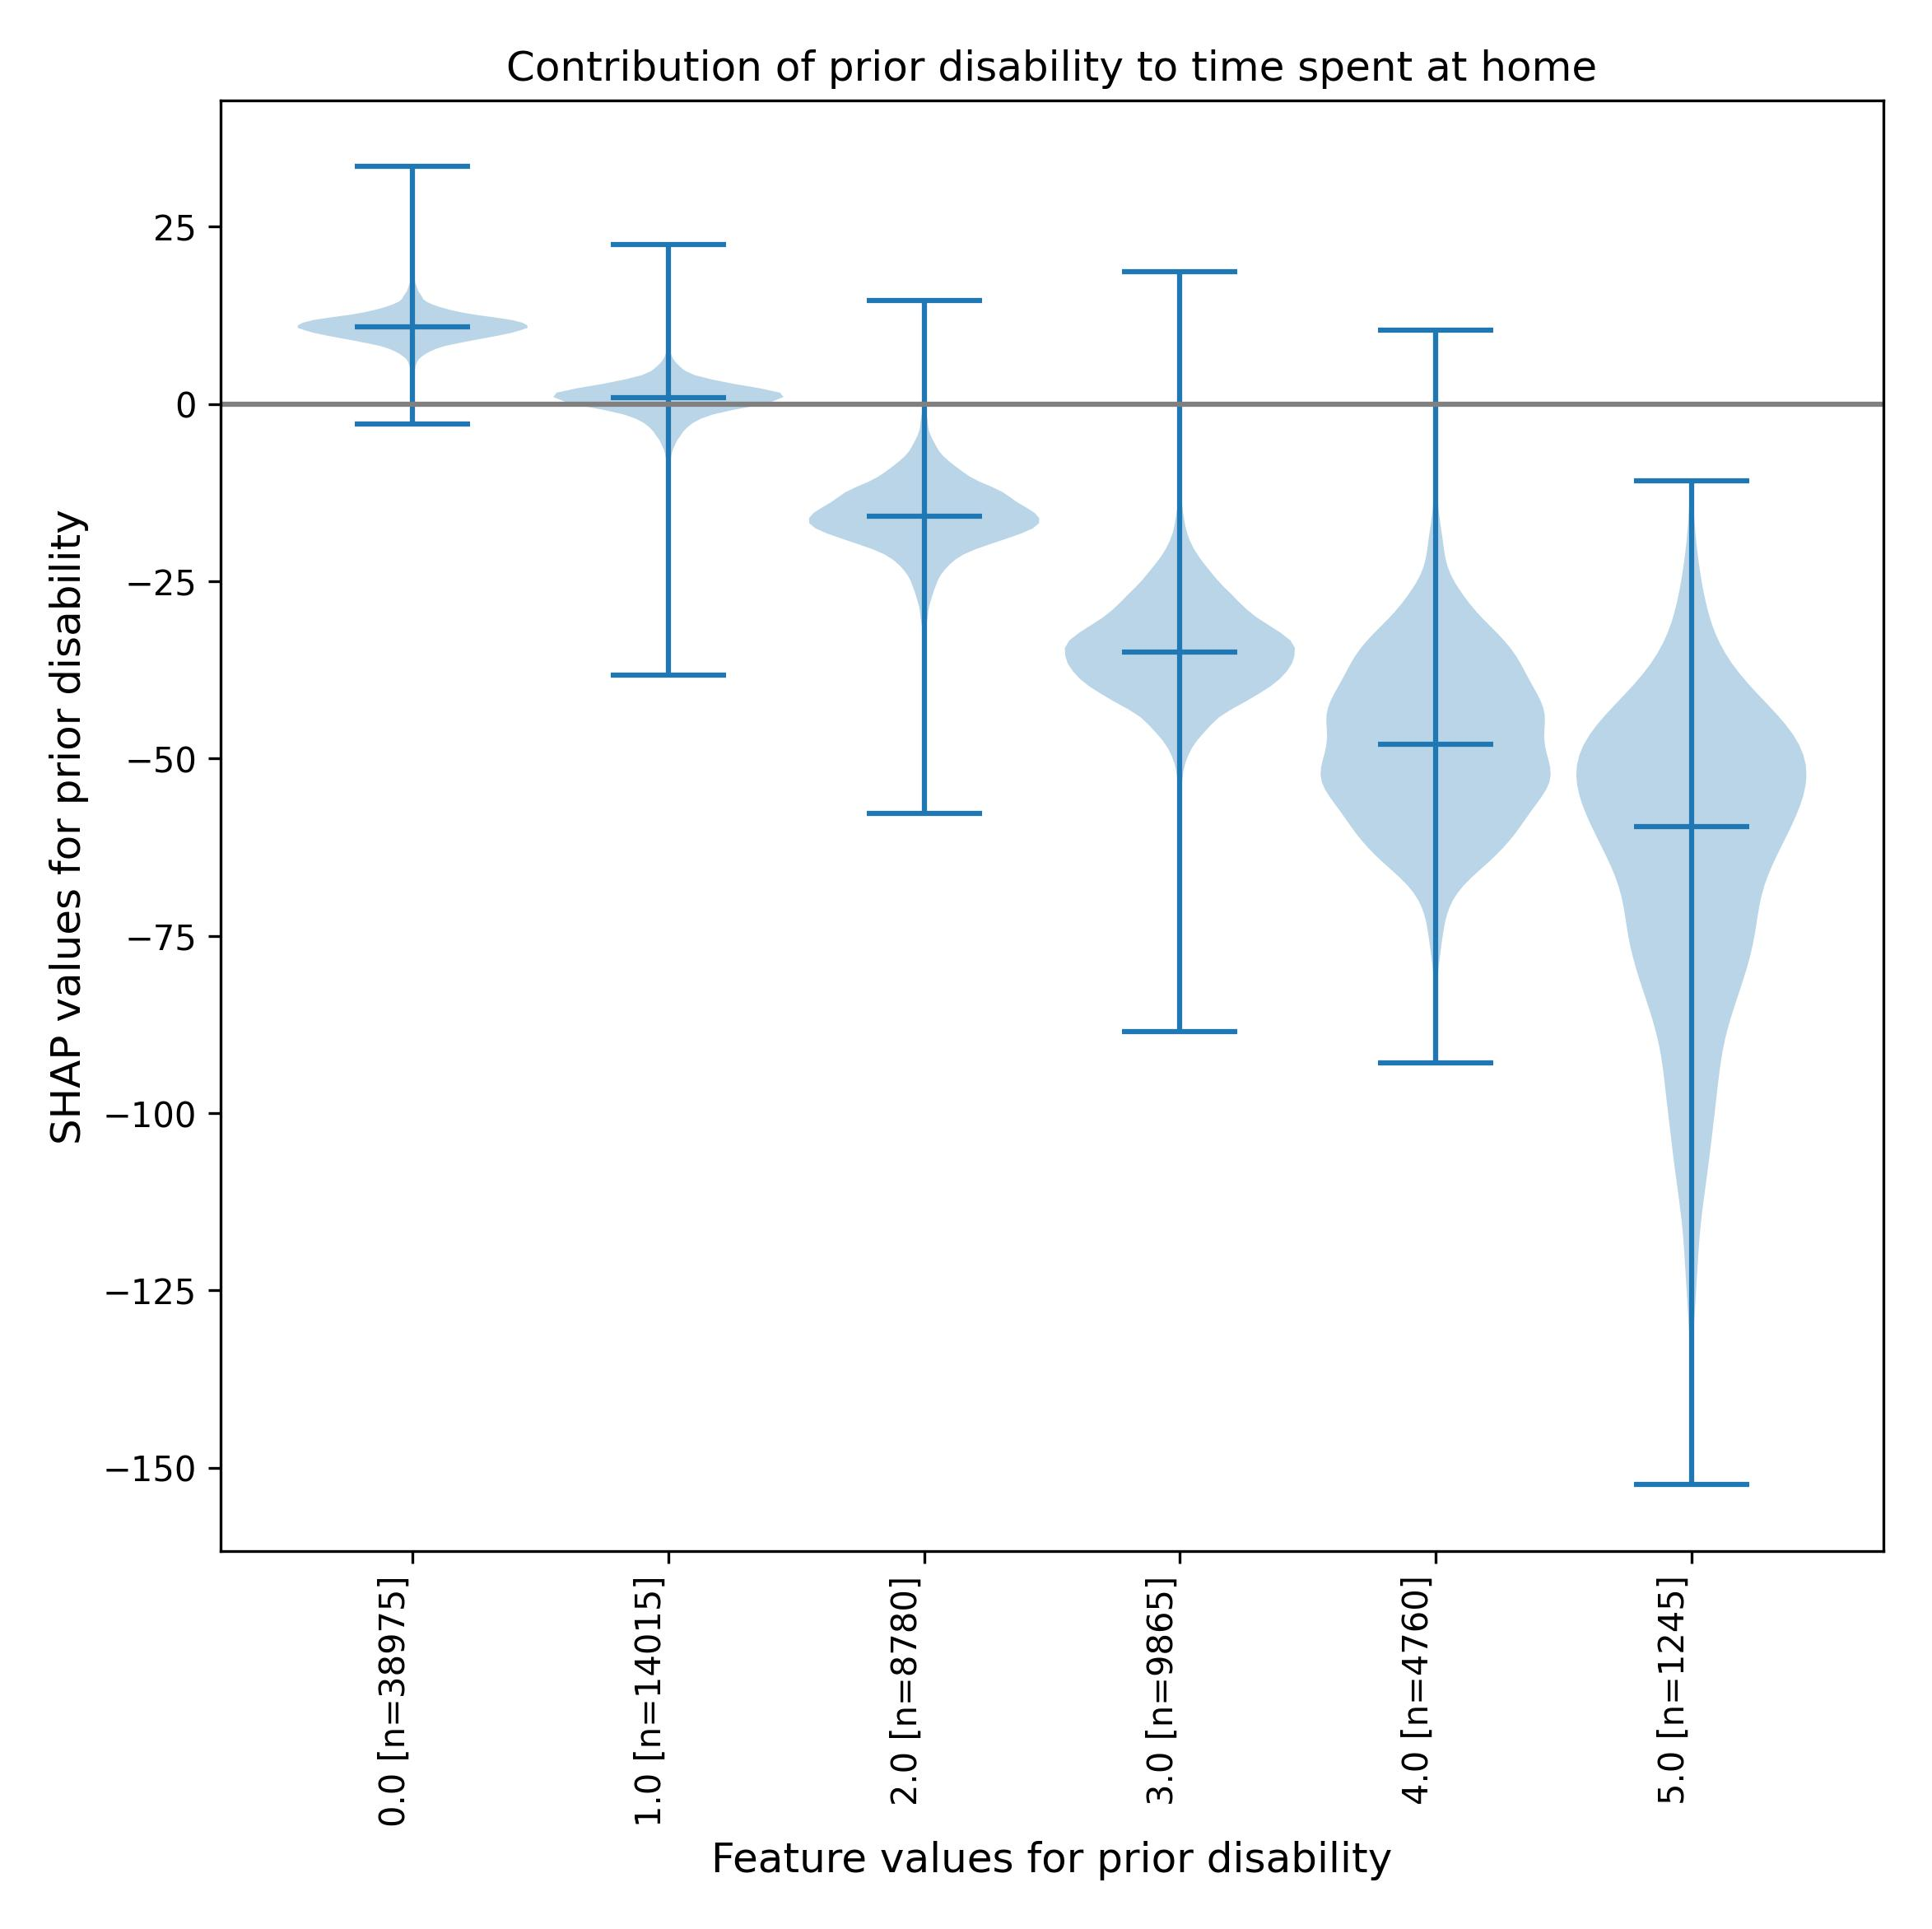
\includegraphics[width=\linewidth]{images/output_results_from_SDE/190_xgboost_at_home_exploratory_population_12_features_violin_shap_prior_disability_kfold0.jpg}
        \caption{At home}
        \label{fig:sub5}
    \end{subfigure}
    \hfill
    \begin{subfigure}[t]{0.31\textwidth}
        \centering
        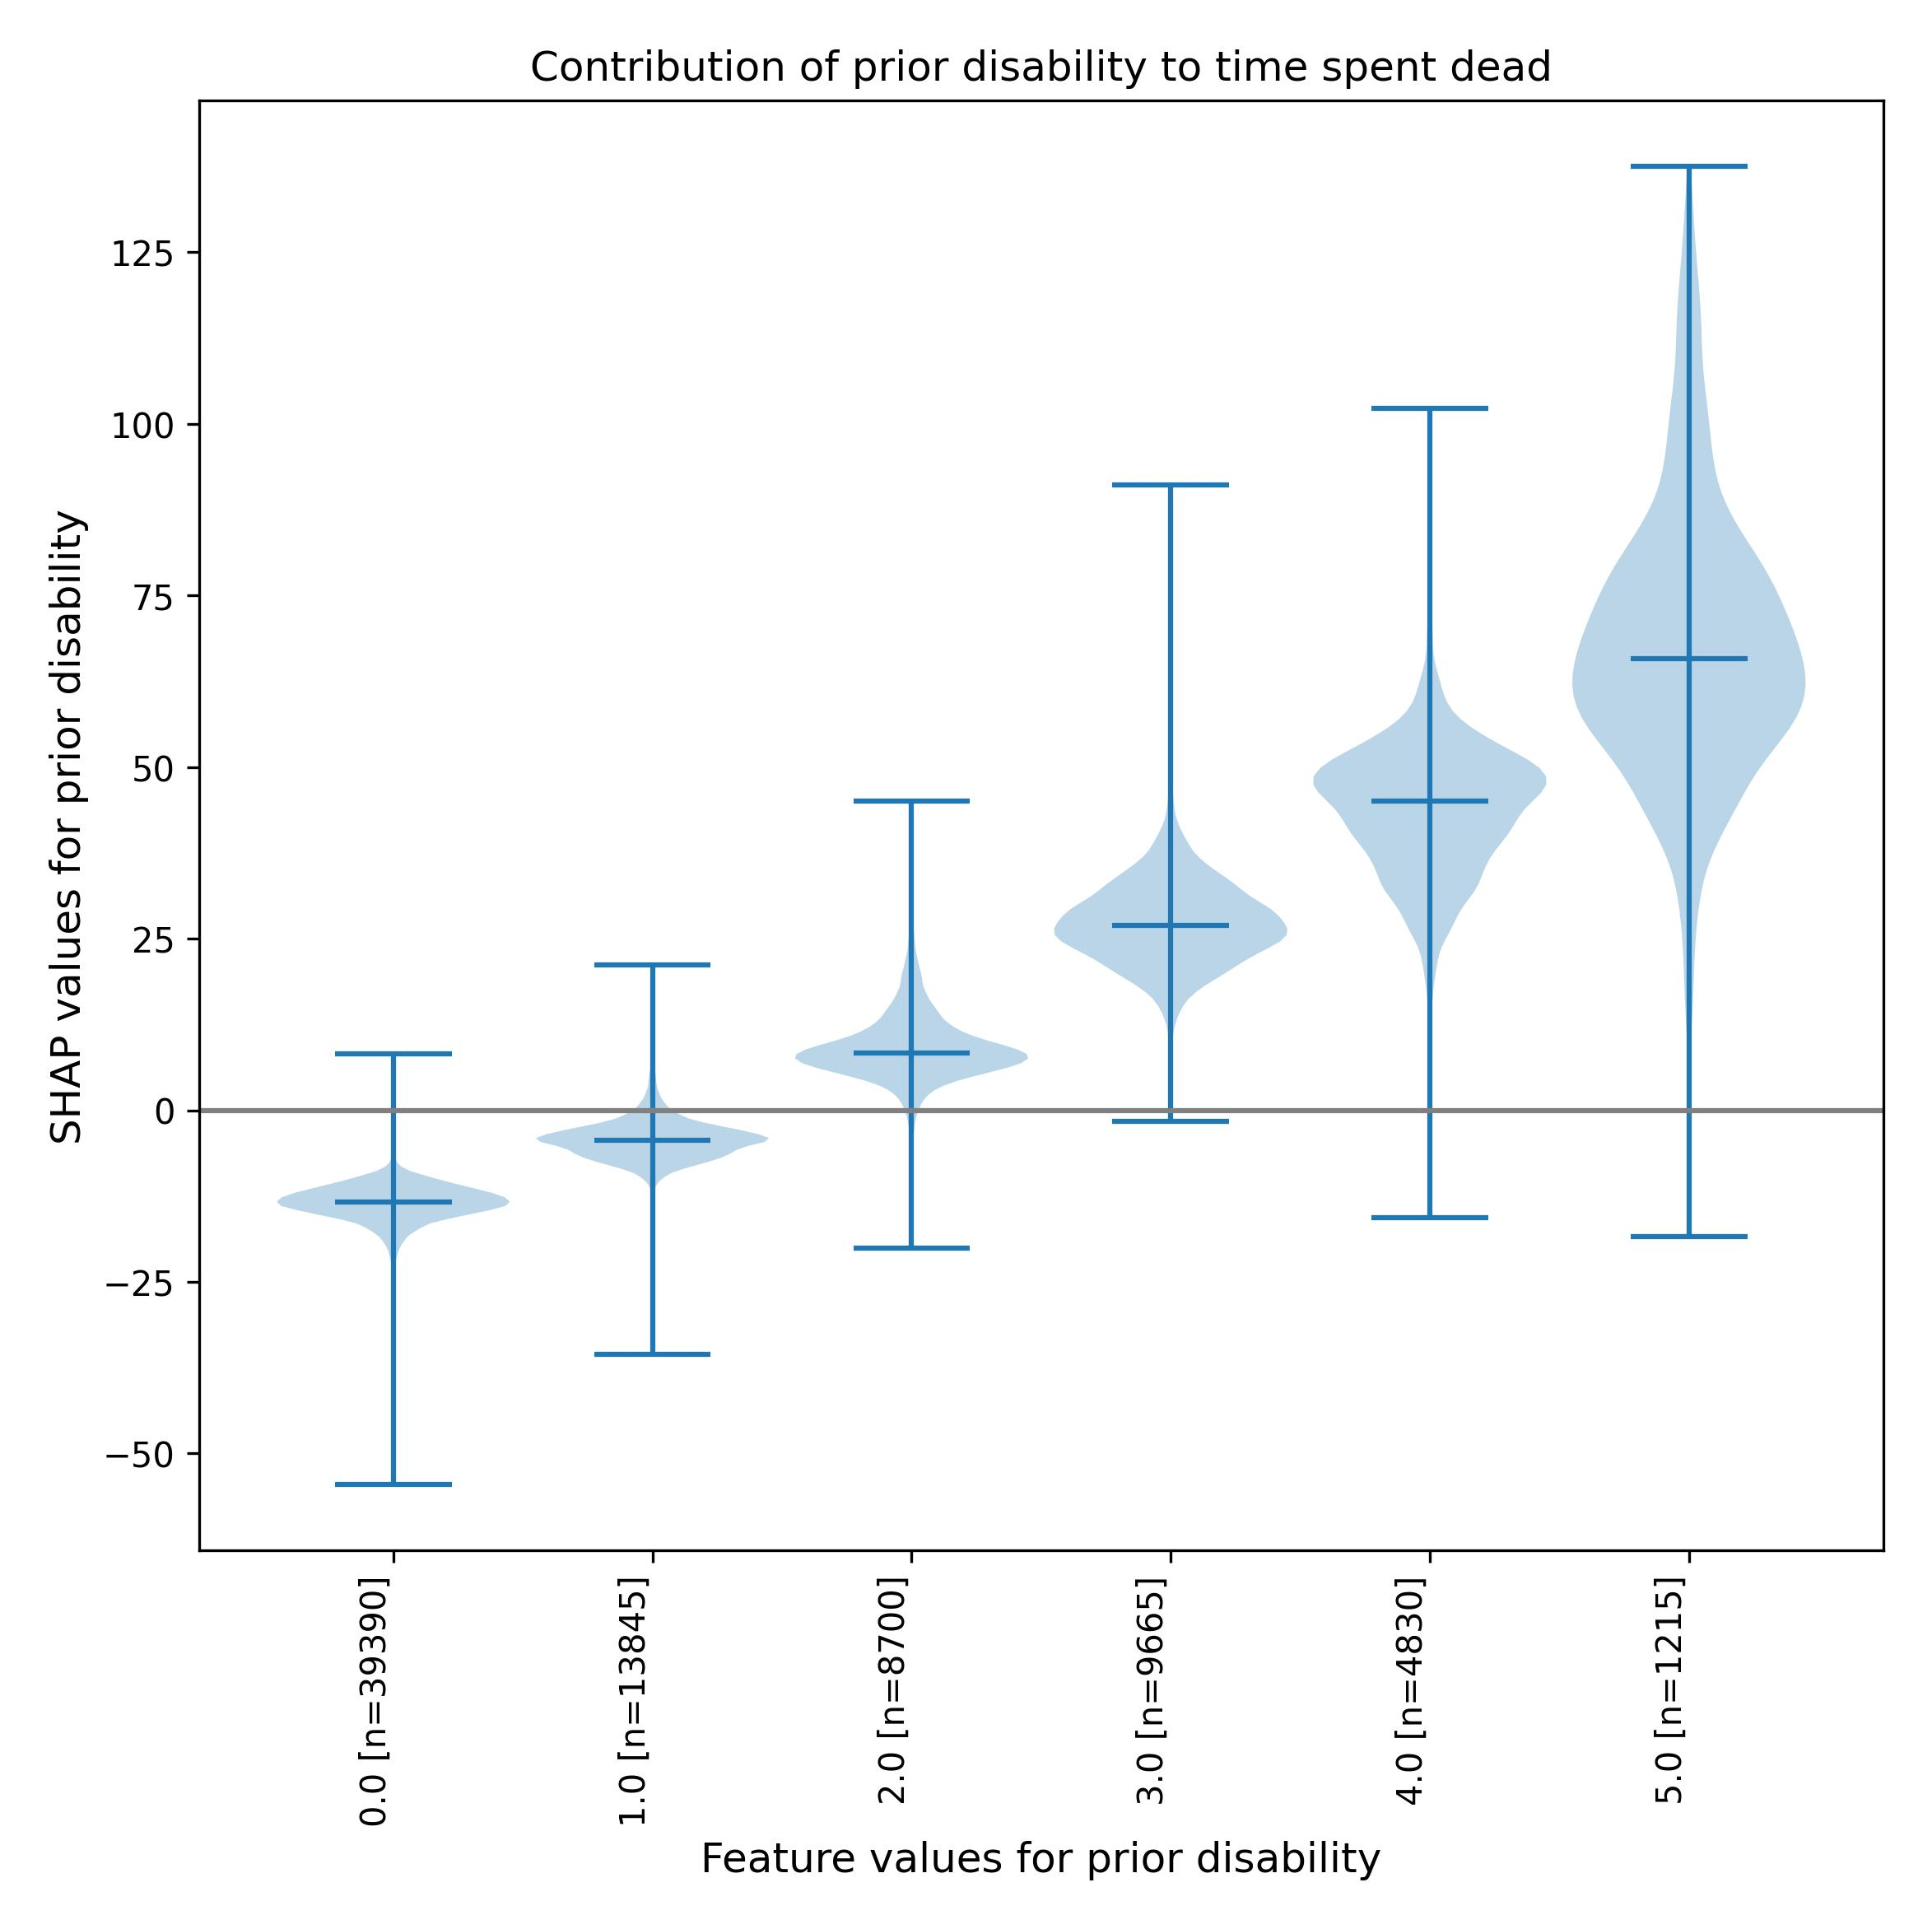
\includegraphics[width=\linewidth]{images/output_results_from_SDE/200_xgboost_dead_exploratory_population_12_features_violin_shap_prior_disability_kfold0.jpg}
        \caption{Dead}
        \label{fig:sub6}
    \end{subfigure}
    \caption*{Prior disability}

    \vspace{2em}

    % ---------- Row 3 ----------
    \begin{subfigure}[t]{0.31\textwidth}
        \centering
        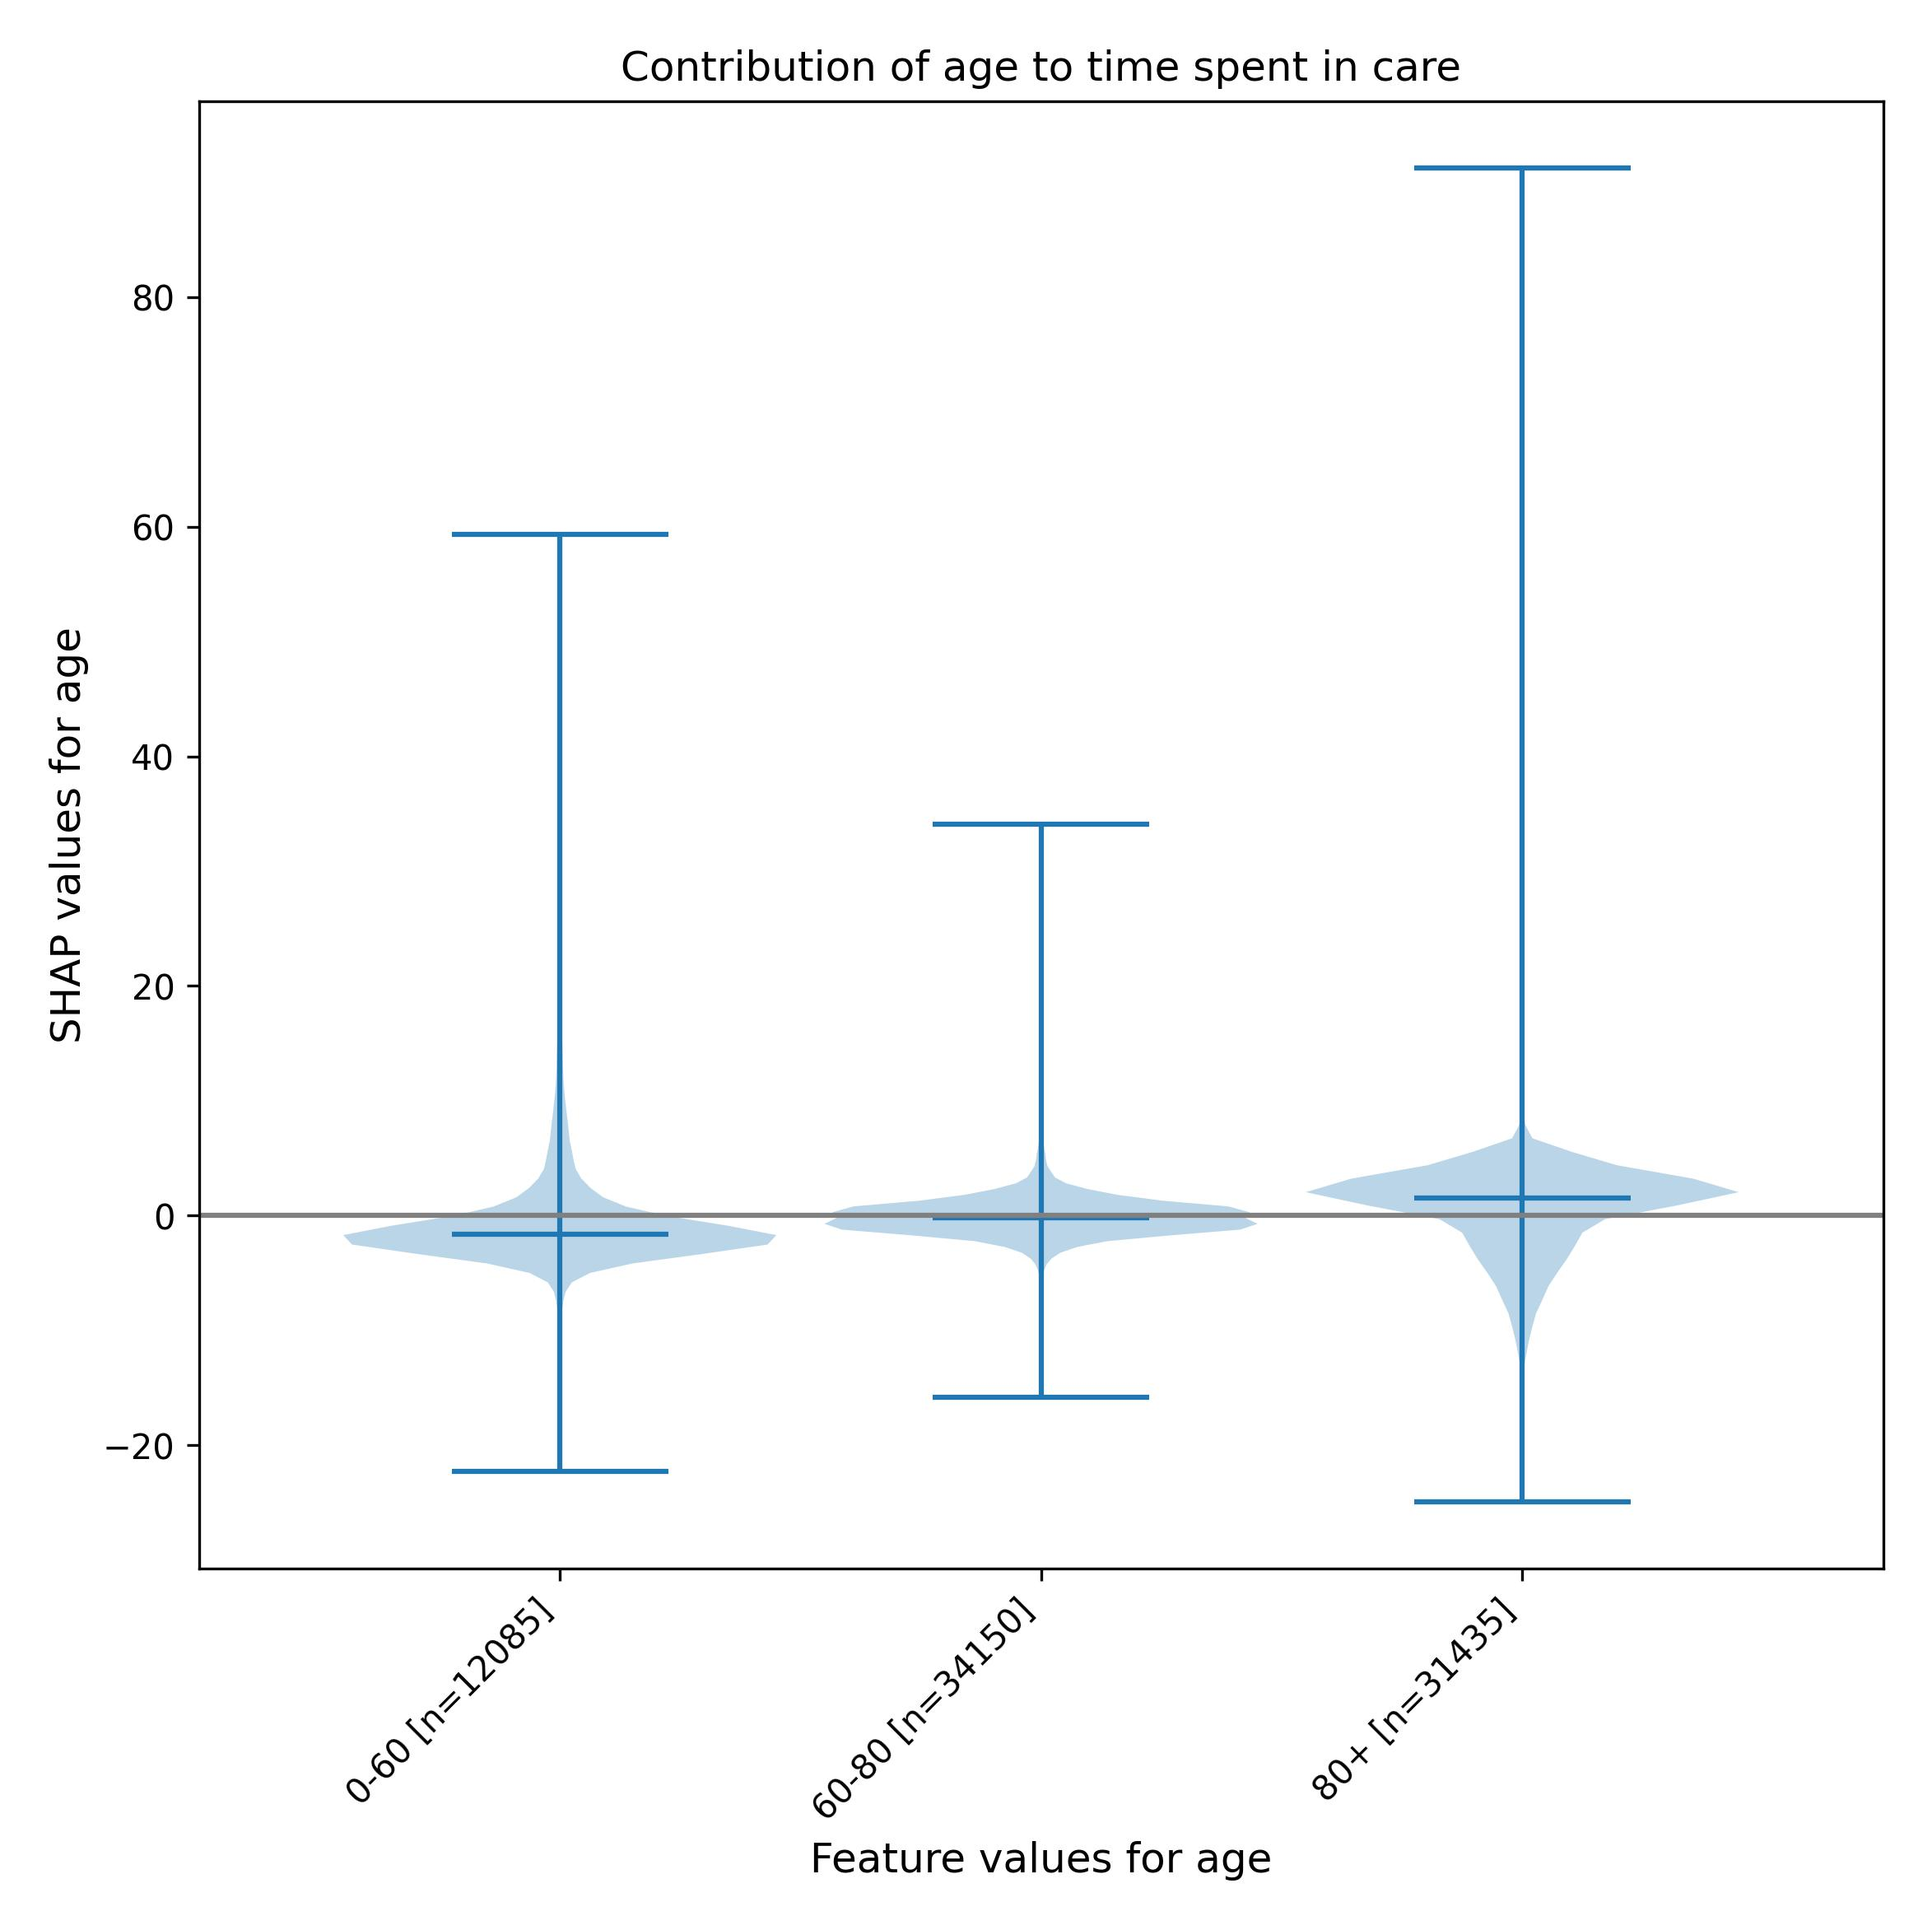
\includegraphics[width=\linewidth]{images/output_results_from_SDE/180_xgboost_in_care_exploratory_population_12_features_violin_shap_age_kfold0.jpg}
        \caption{In care}
        \label{fig:sub7}
    \end{subfigure}
    \hfill
    \begin{subfigure}[t]{0.31\textwidth}
        \centering
        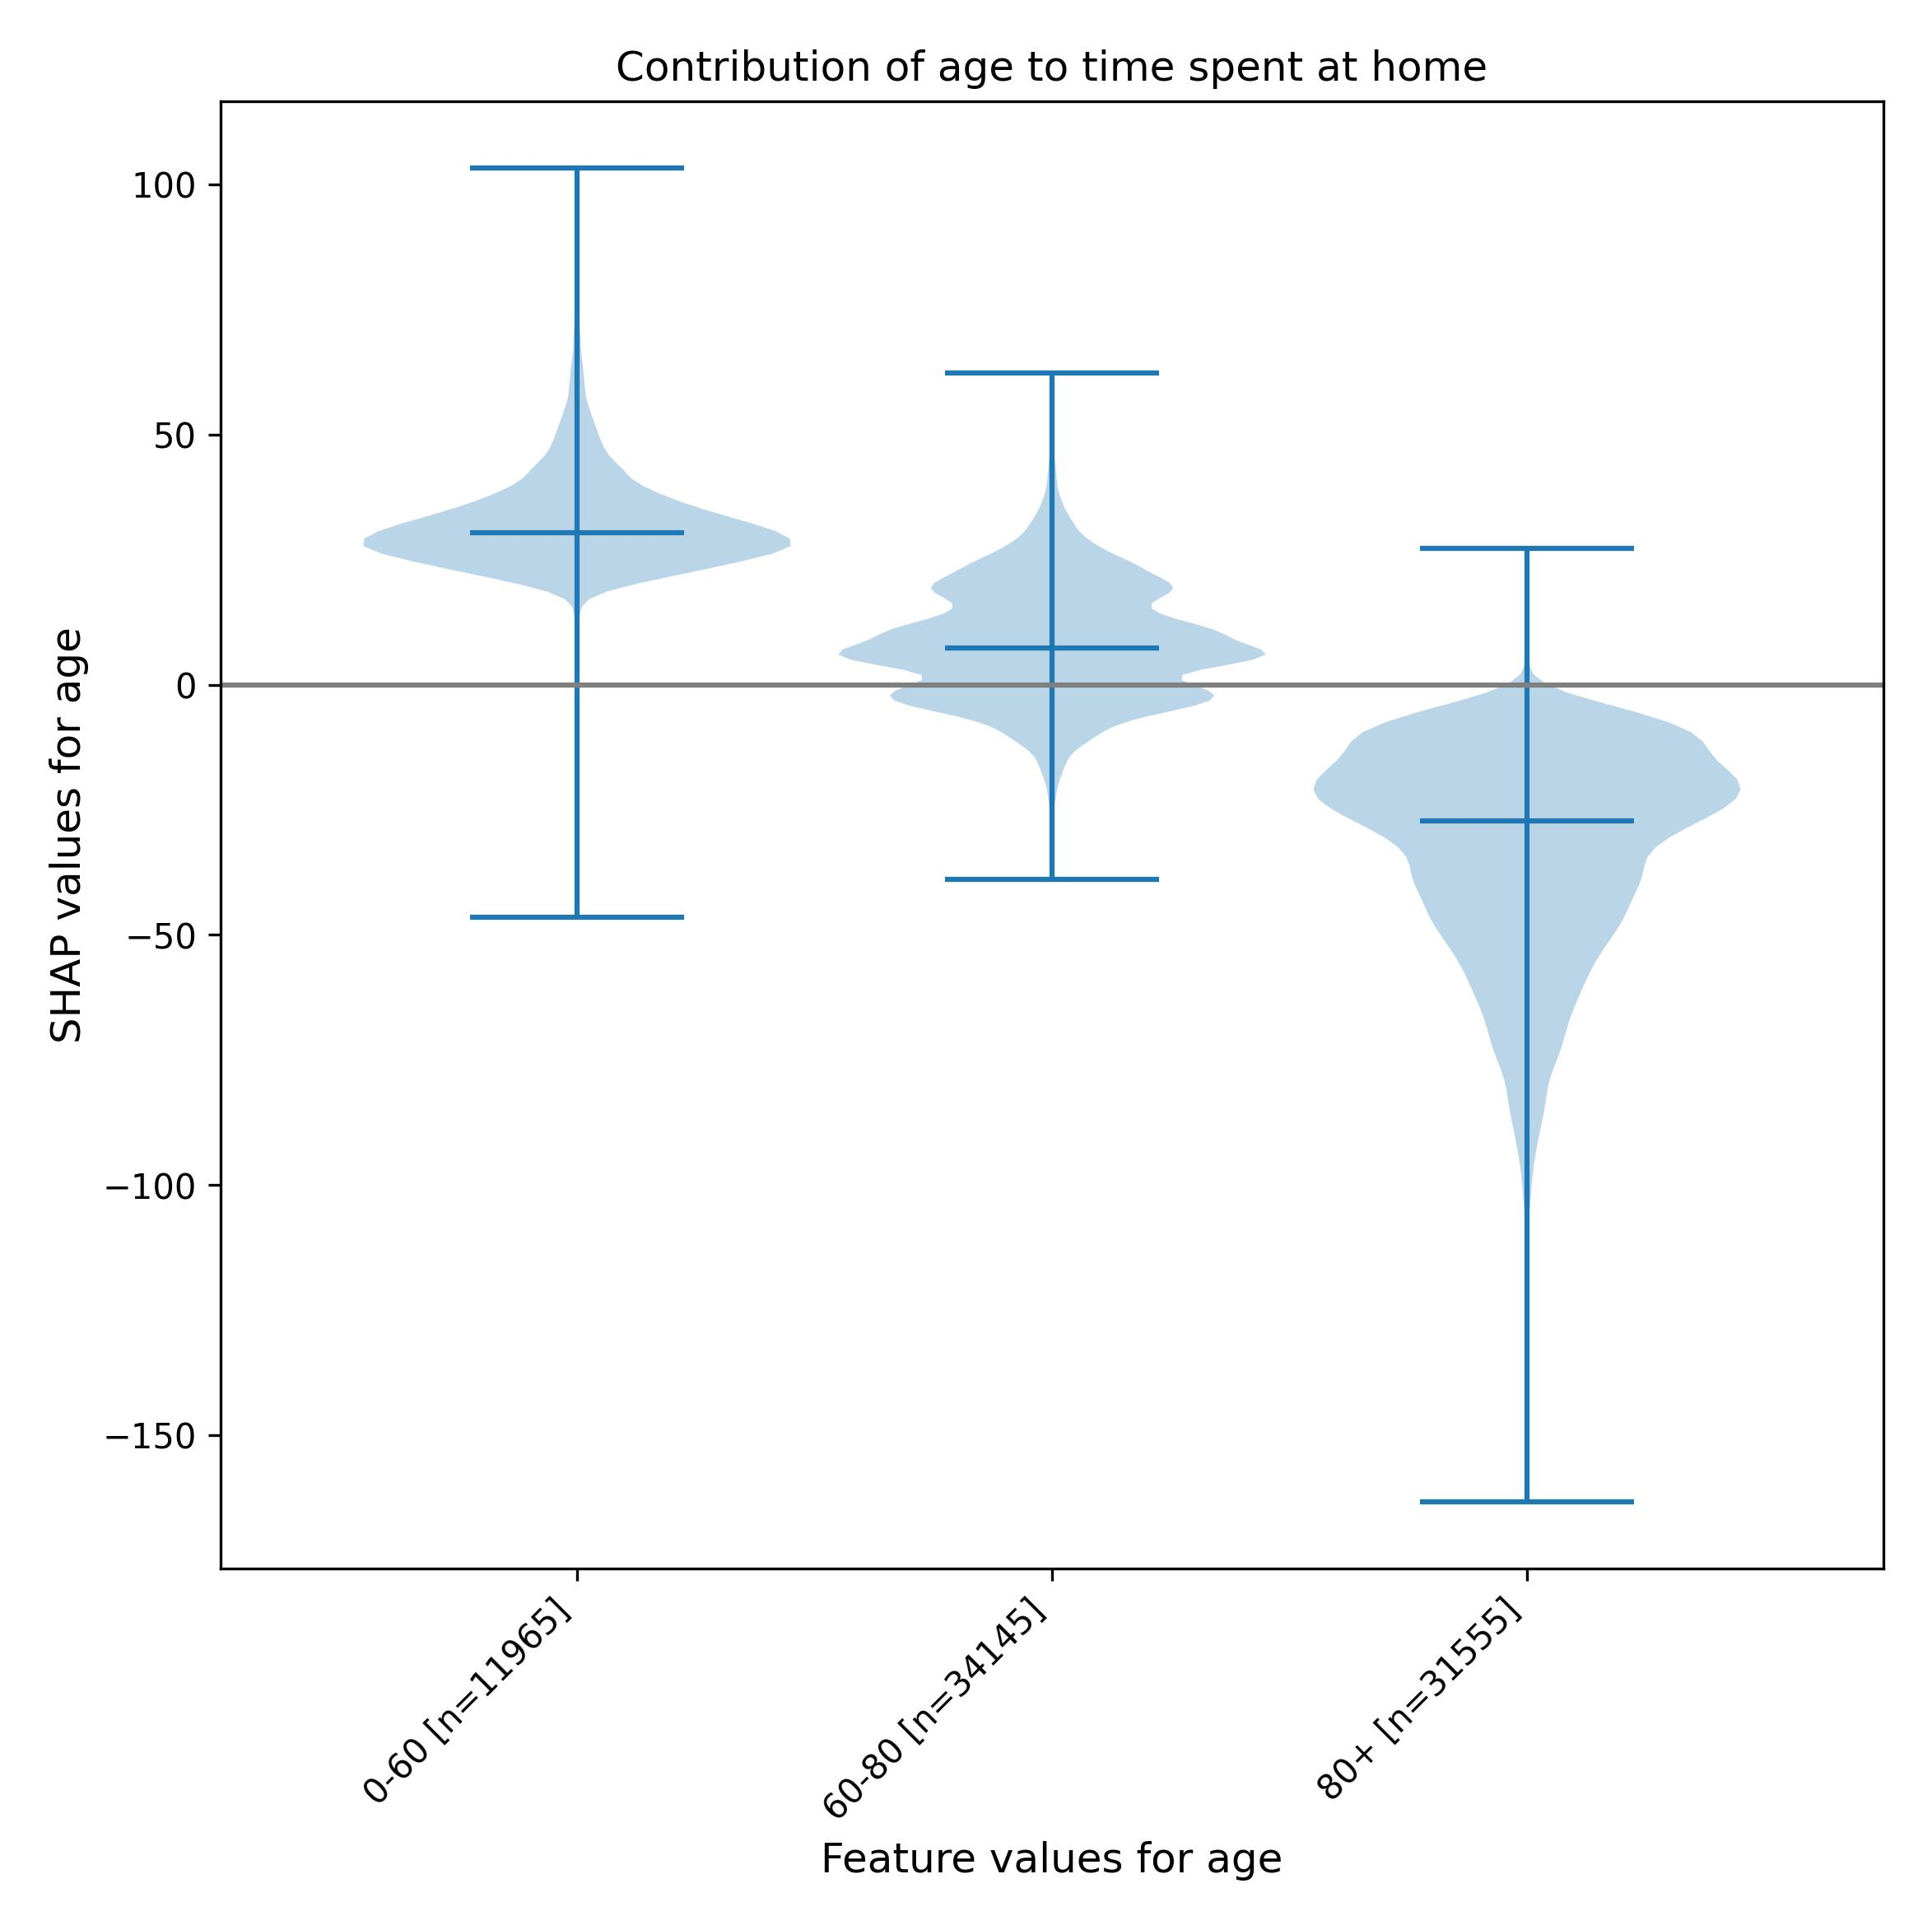
\includegraphics[width=\linewidth]{images/output_results_from_SDE/190_xgboost_at_home_exploratory_population_12_features_violin_shap_age_kfold0.jpg}
        \caption{At home}
        \label{fig:sub8}
    \end{subfigure}
    \hfill
    \begin{subfigure}[t]{0.31\textwidth}
        \centering
        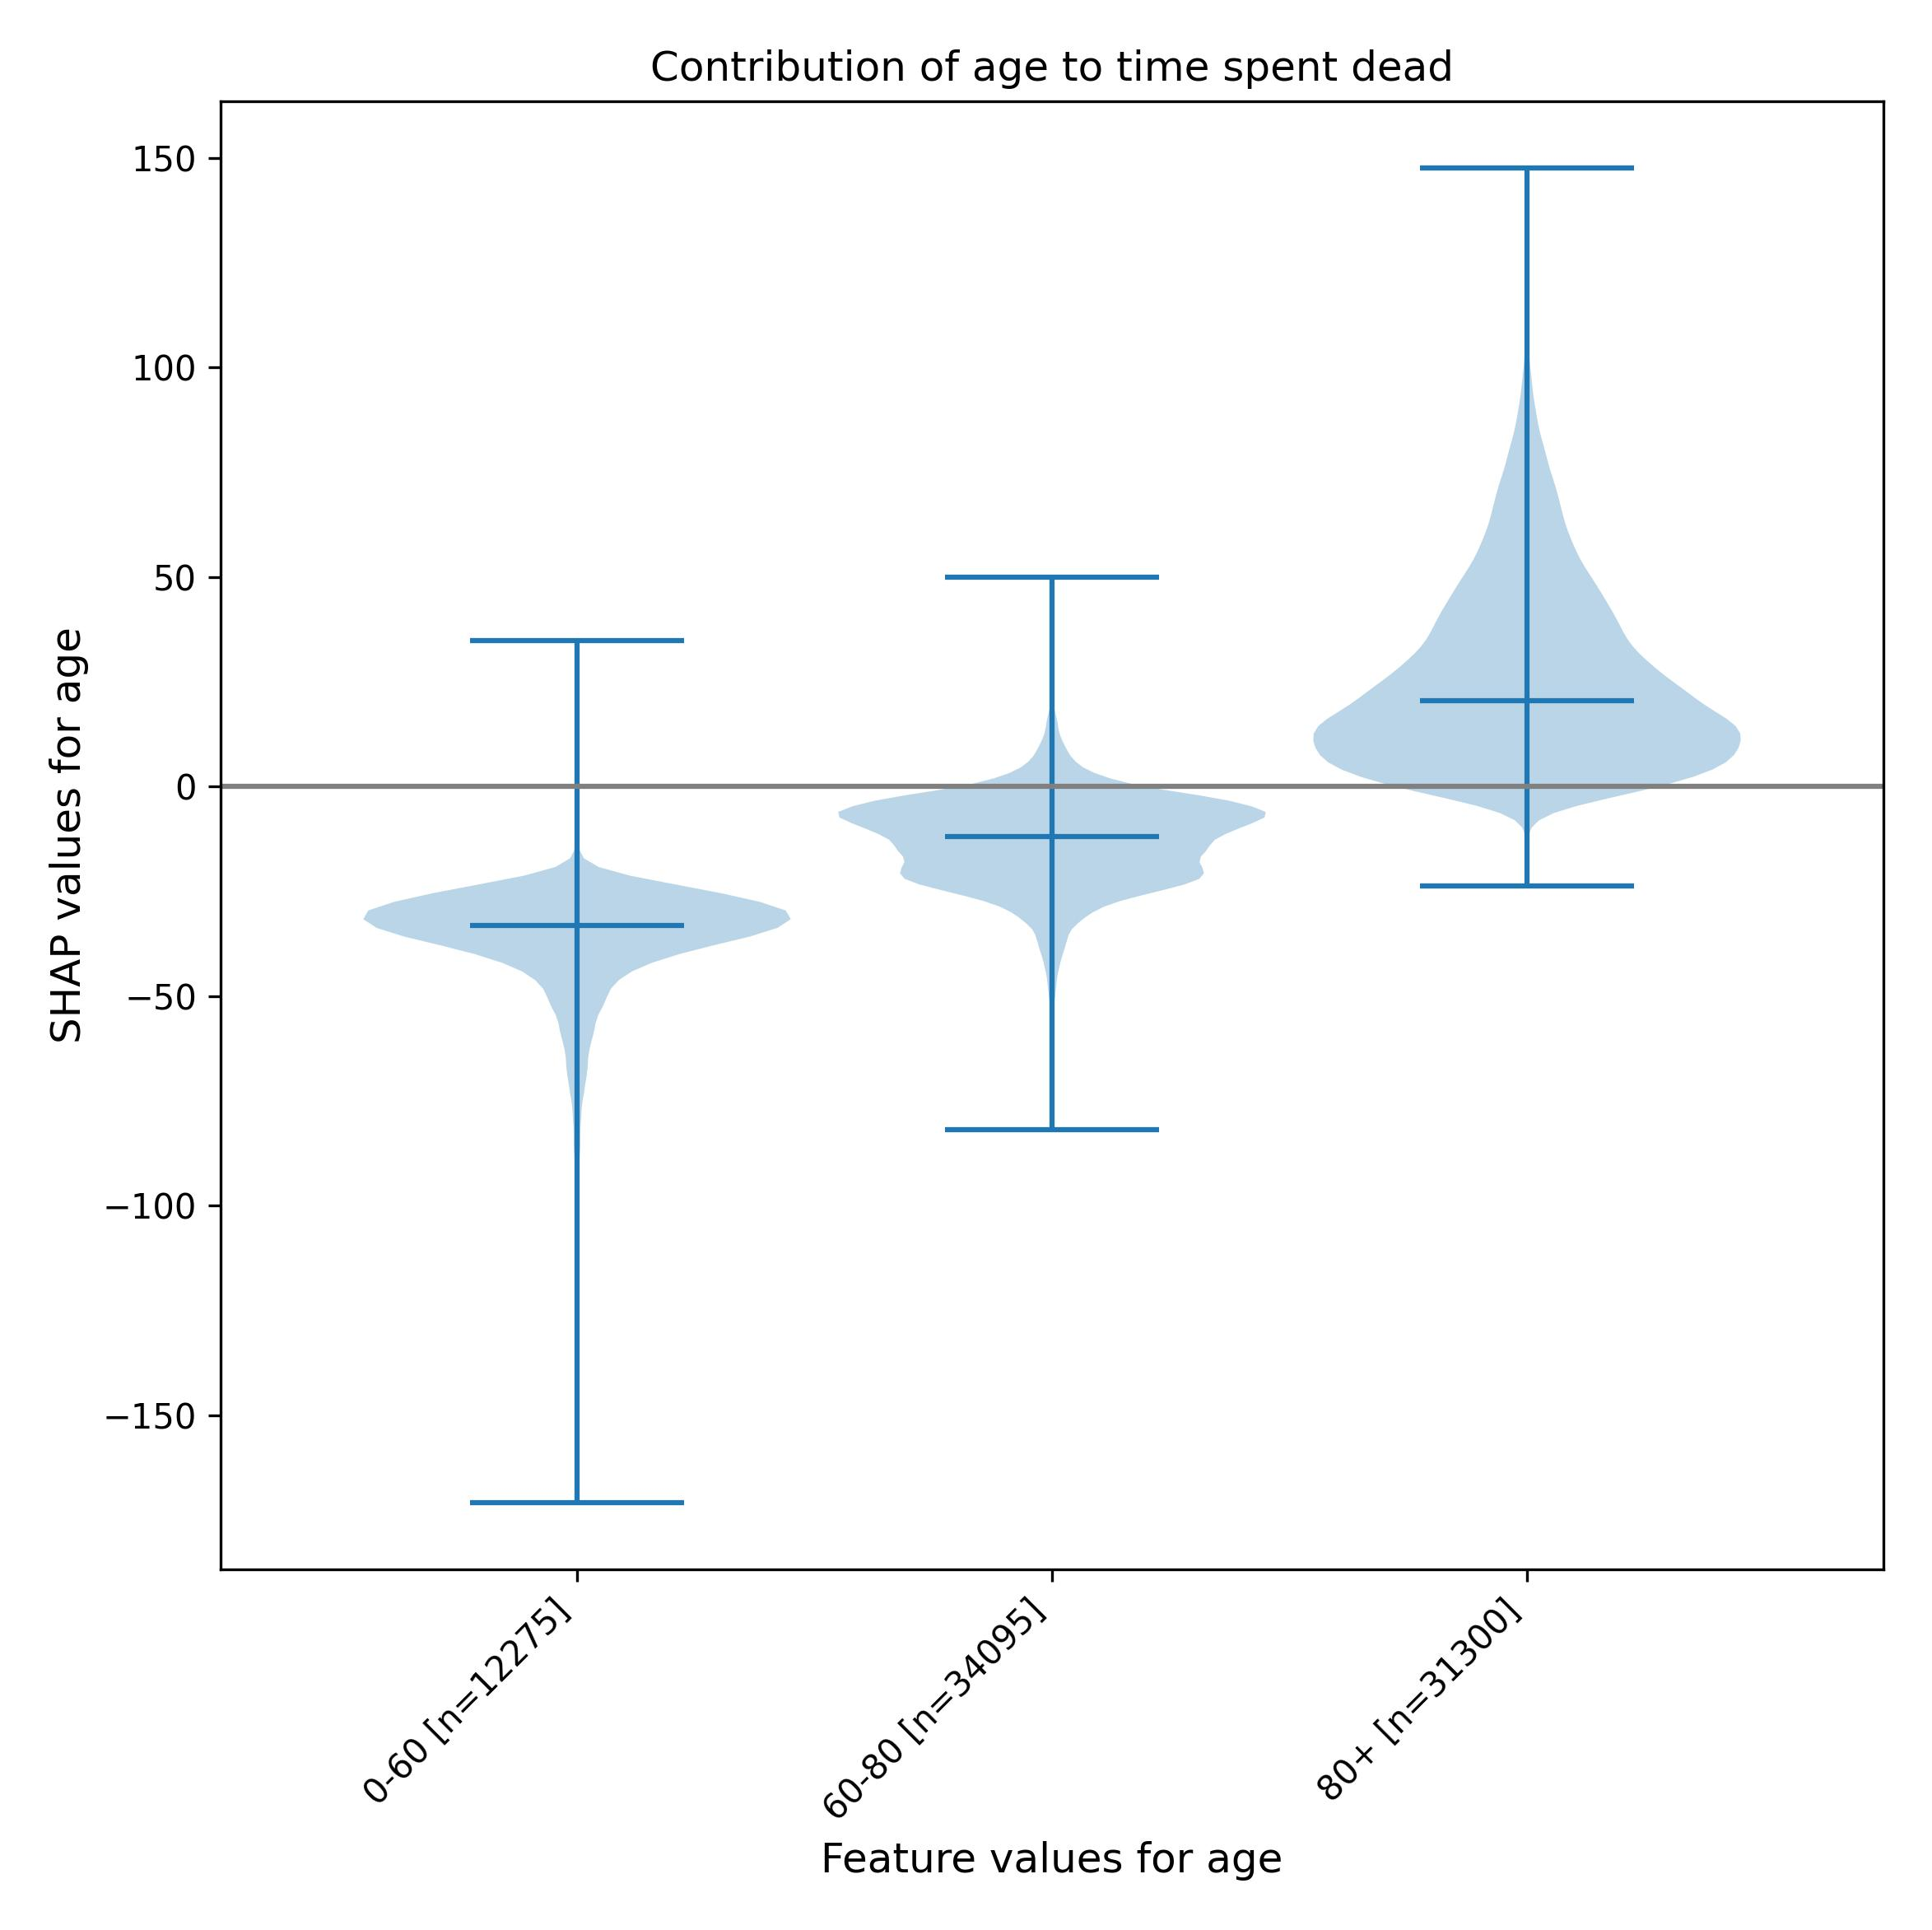
\includegraphics[width=\linewidth]{images/output_results_from_SDE/200_xgboost_dead_exploratory_population_12_features_violin_shap_age_kfold0.jpg}
        \caption{Dead}
        \label{fig:sub9}
    \end{subfigure}
    \caption*{Age}

    \vspace{2em}

    \caption{SHAP analysis on how feature values influence XGBoost model predictions for time spent in a) NHS inpatient care (left), b) at home (alive, and outside of NHS inpatient care), and c) dead, in the year after stroke. Features shown are stroke severity (NIHSS, top), prior disability (mRS, middle), and age group (bottom). SHAP values are calculated for each prediction, taking into account interactions with other features. The resulting distributions for any given feature value are shown in the figure as violin plots with median and range bars.}
    \label{fig:shap_1}
\end{figure}

%%%%%%%%%%%%%%%%%%%%%%%%%%%%%%%%%%%%%%%%%%%%%%%%%%%%%%%%%%%%%%%%%%%%

\begin{figure}[htbp]
    \centering

    % ---------- Row 1 ----------
    
    \begin{subfigure}[t]{0.31\textwidth}
        \centering
        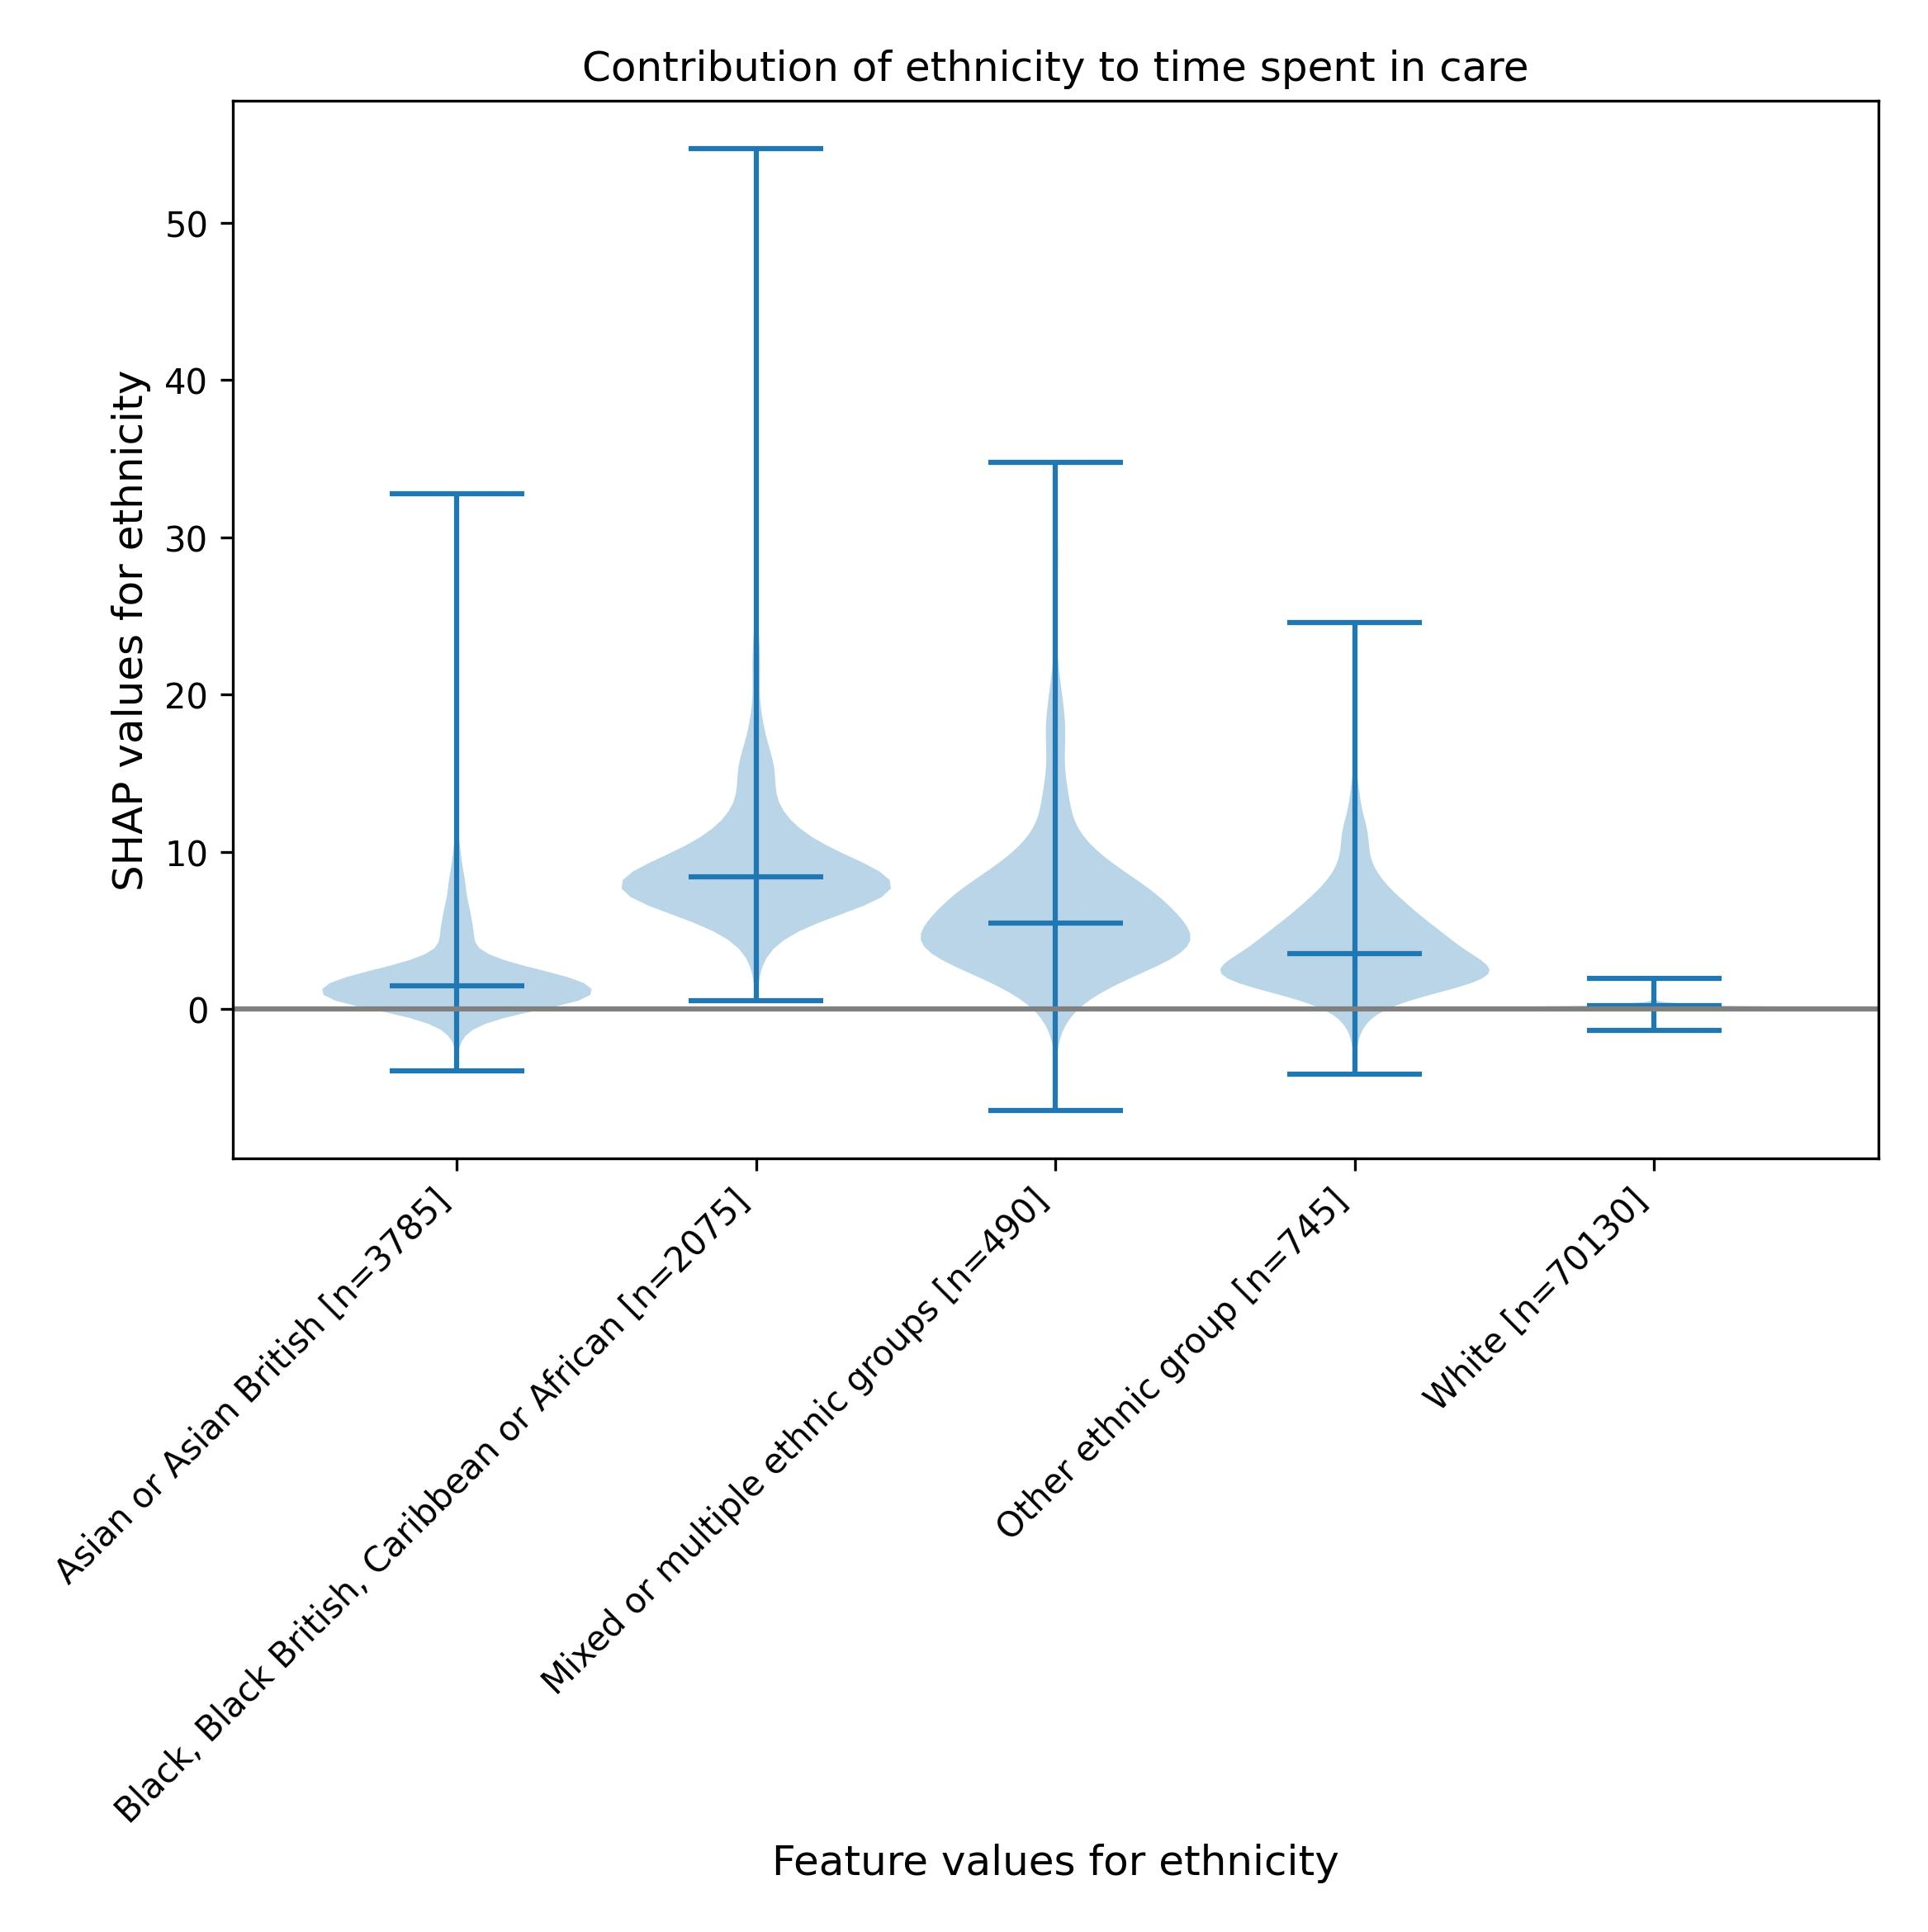
\includegraphics[width=\linewidth]{images/output_results_from_SDE/180_xgboost_in_care_exploratory_population_12_features_shap_violin_ethnicity_kfold0.jpg}
        \caption{In care}
        \label{fig:sub1}
    \end{subfigure}
    \hfill
    \begin{subfigure}[t]{0.31\textwidth}
        \centering
        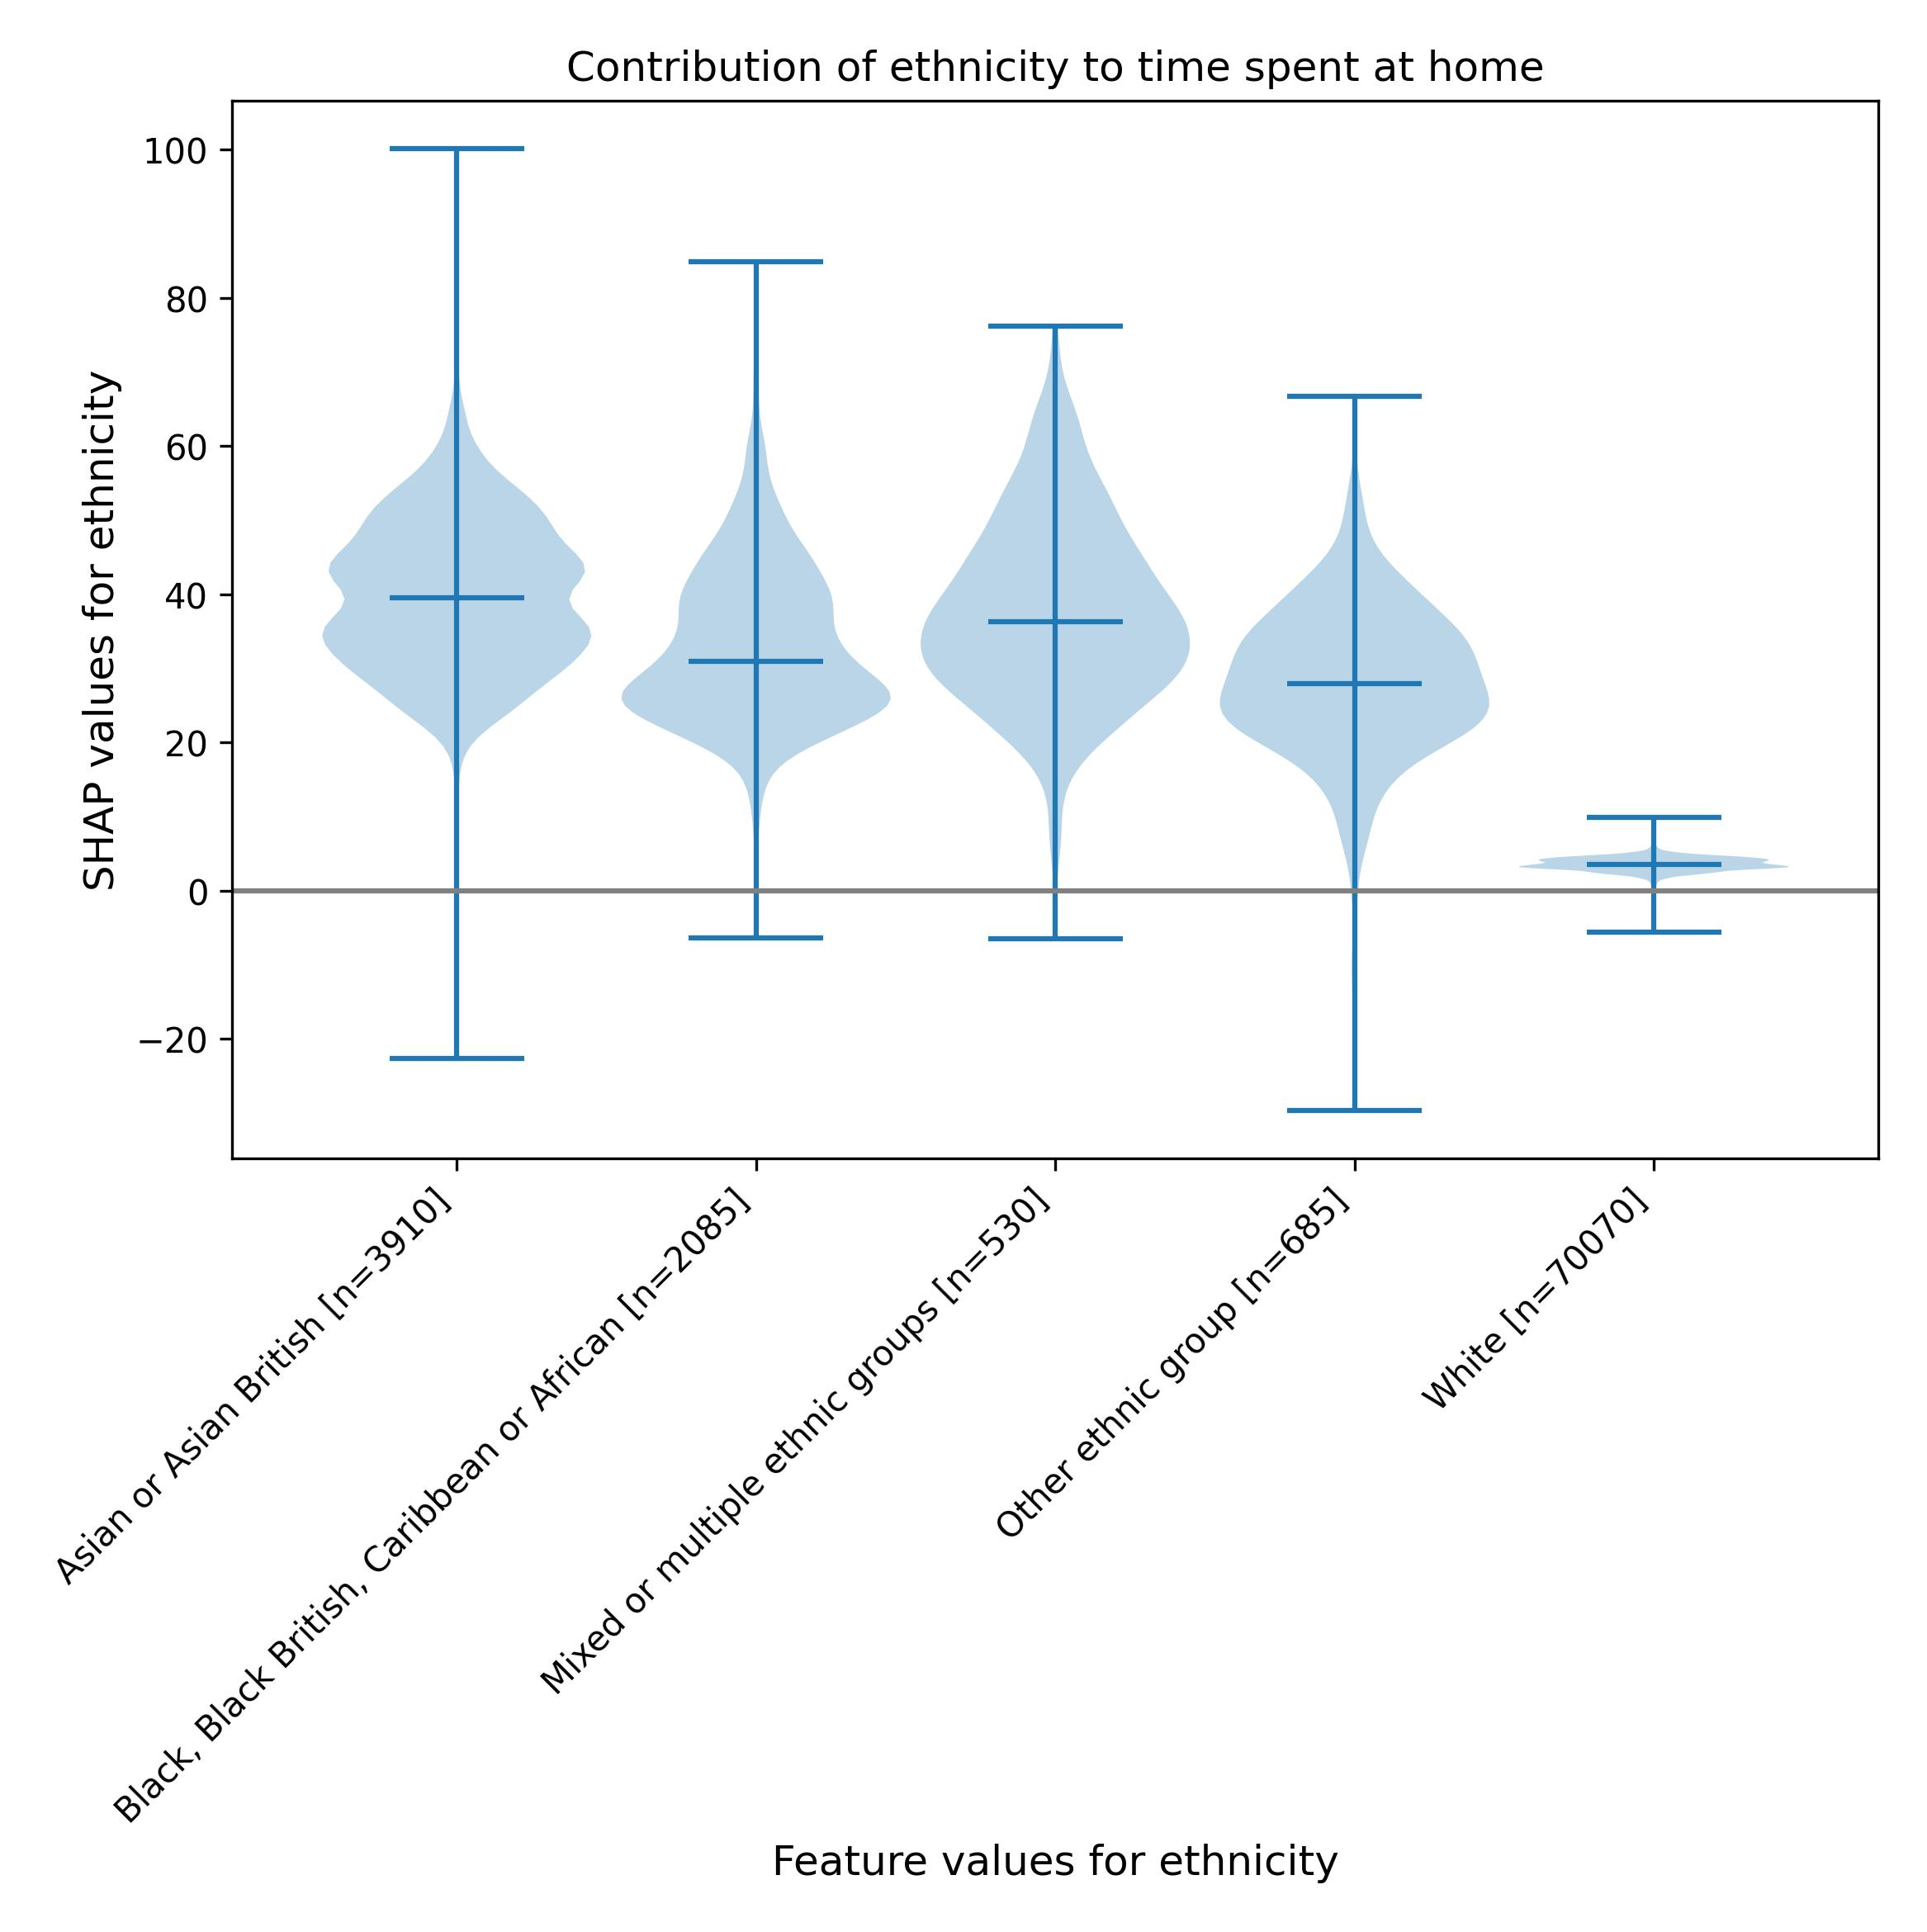
\includegraphics[width=\linewidth]{images/output_results_from_SDE/190_xgboost_at_home_exploratory_population_12_features_shap_violin_ethnicity_kfold0.jpg}
        \caption{At home}
        \label{fig:sub2}
    \end{subfigure}
    \hfill
    \begin{subfigure}[t]{0.31\textwidth}
        \centering
        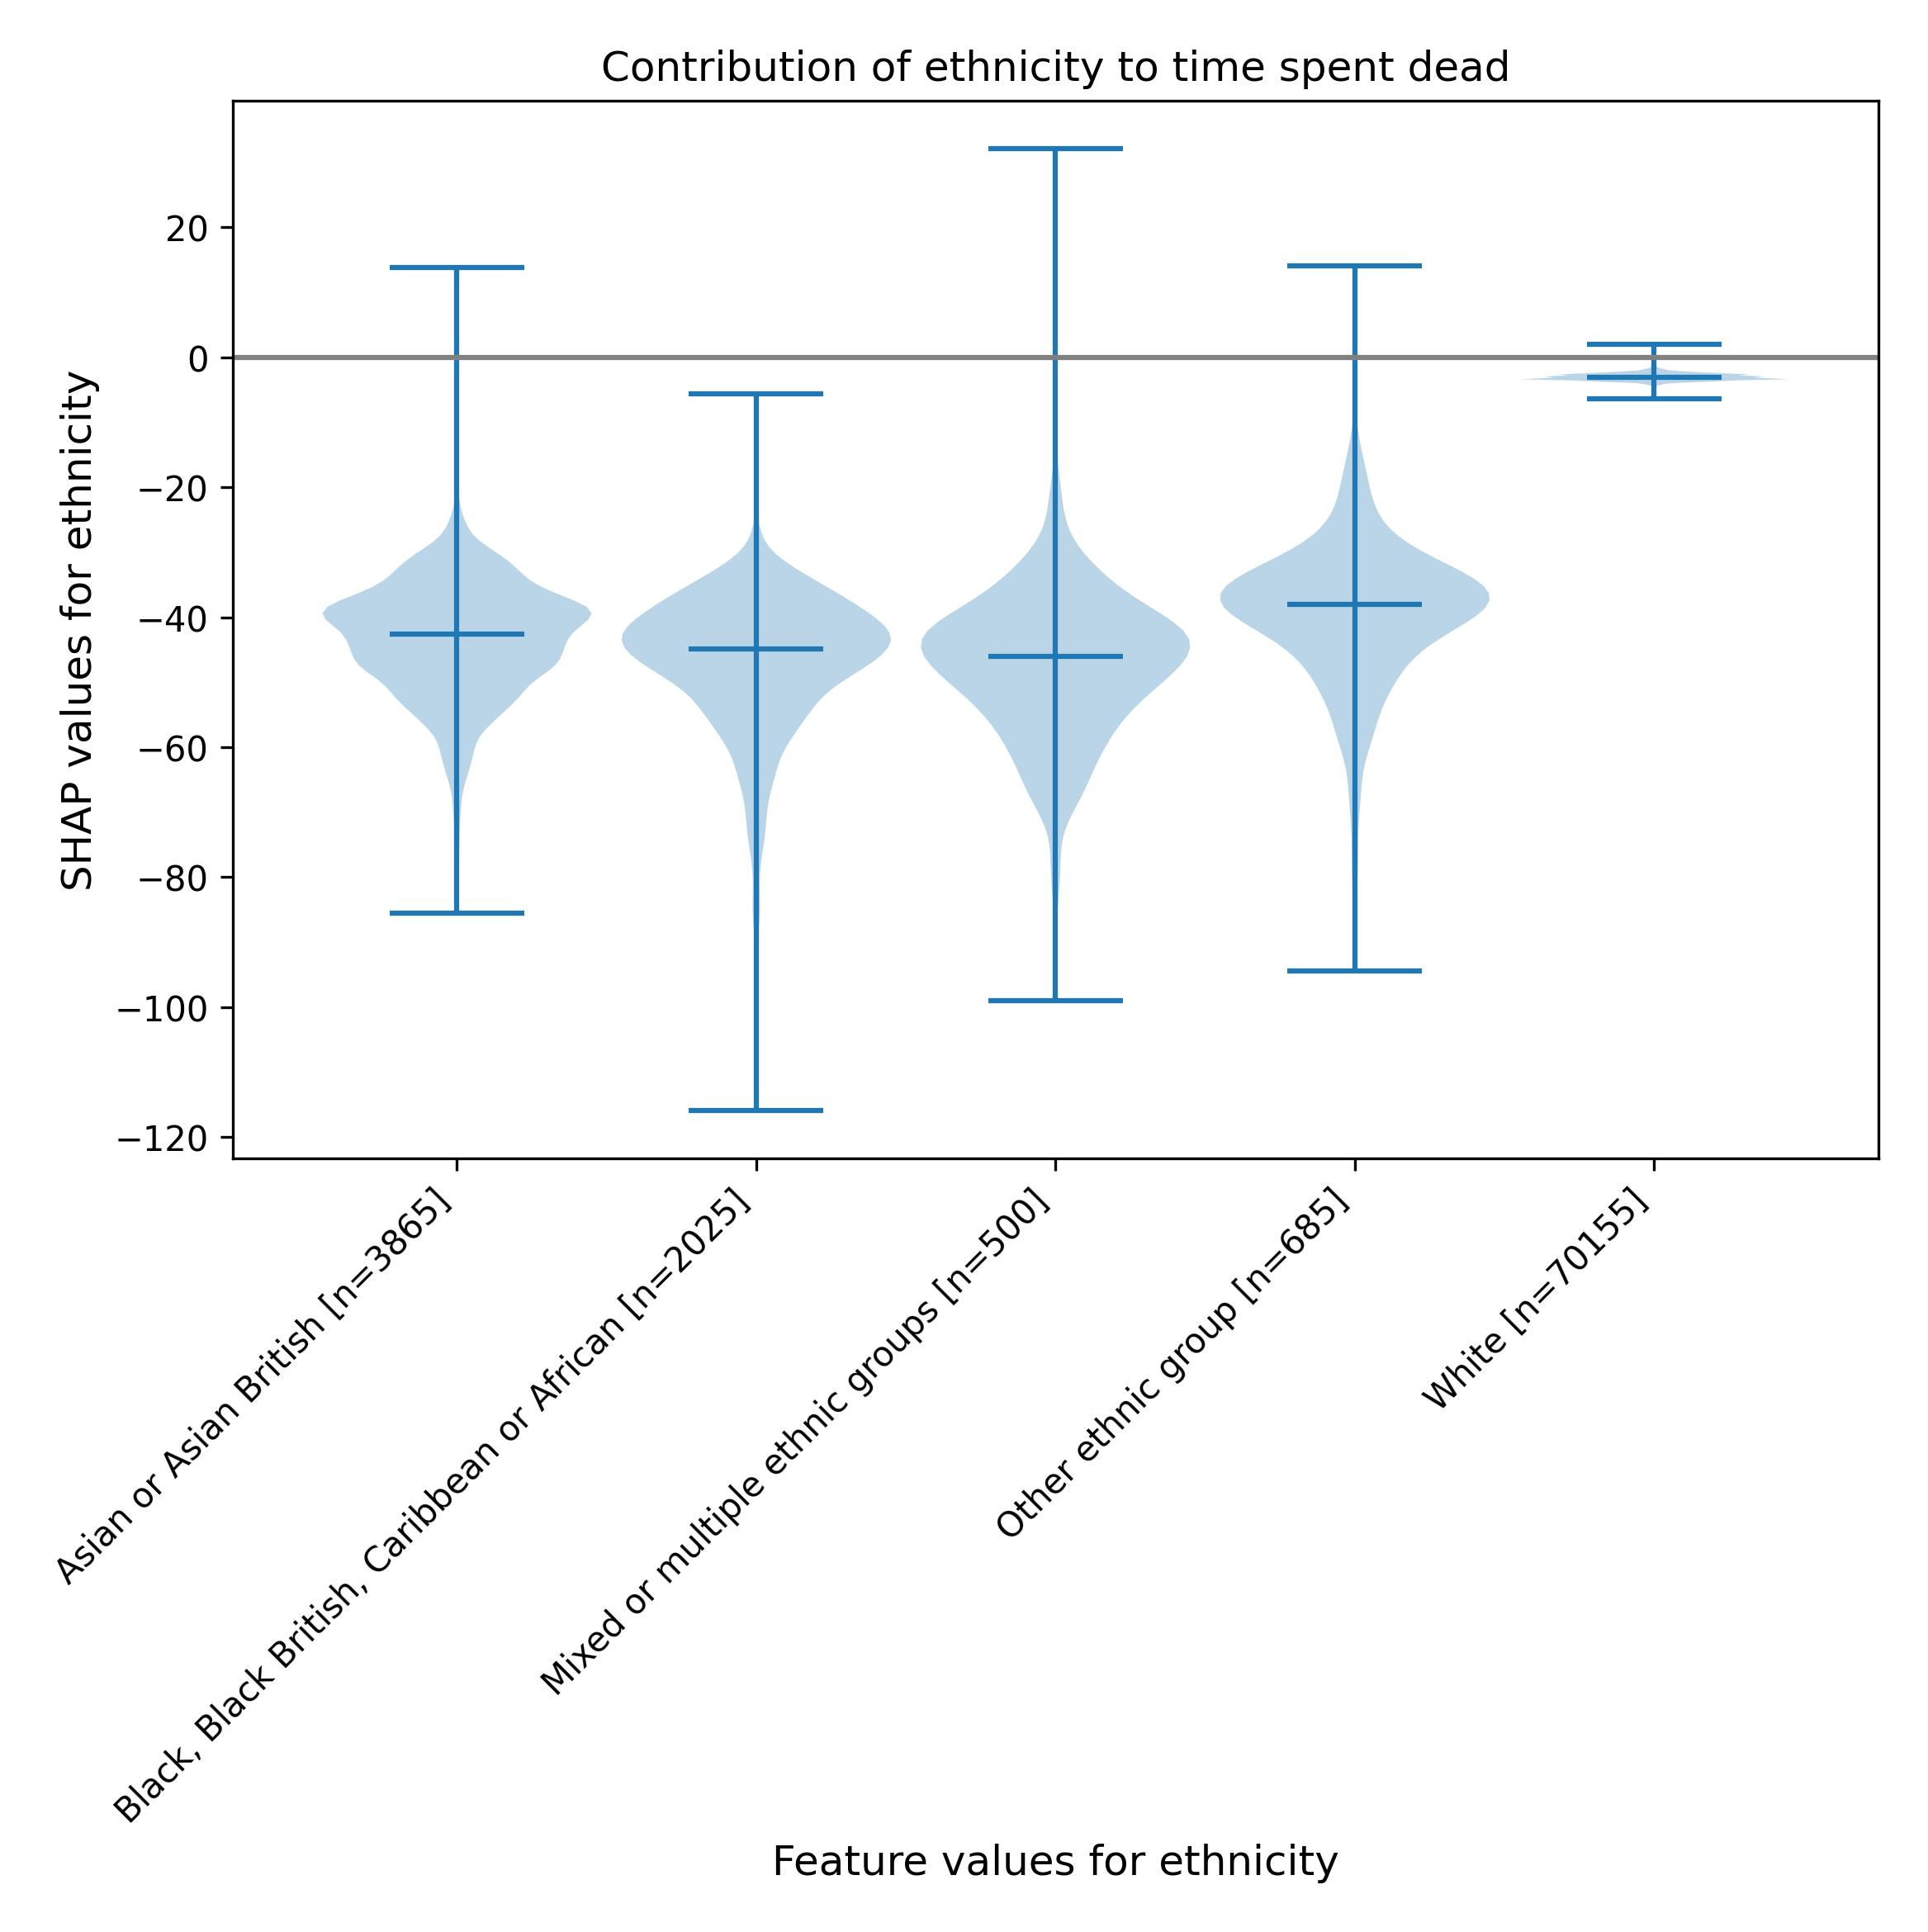
\includegraphics[width=\linewidth]{images/output_results_from_SDE/200_xgboost_dead_exploratory_population_12_features_shap_violin_ethnicity_kfold0.jpg}
        \caption{Dead}
        \label{fig:sub3}
    \end{subfigure}
    \caption*{Ethnicity}

    \vspace{2em} % space between rows

    % ---------- Row 2 ----------
    \begin{subfigure}[t]{0.31\textwidth}
        \centering
        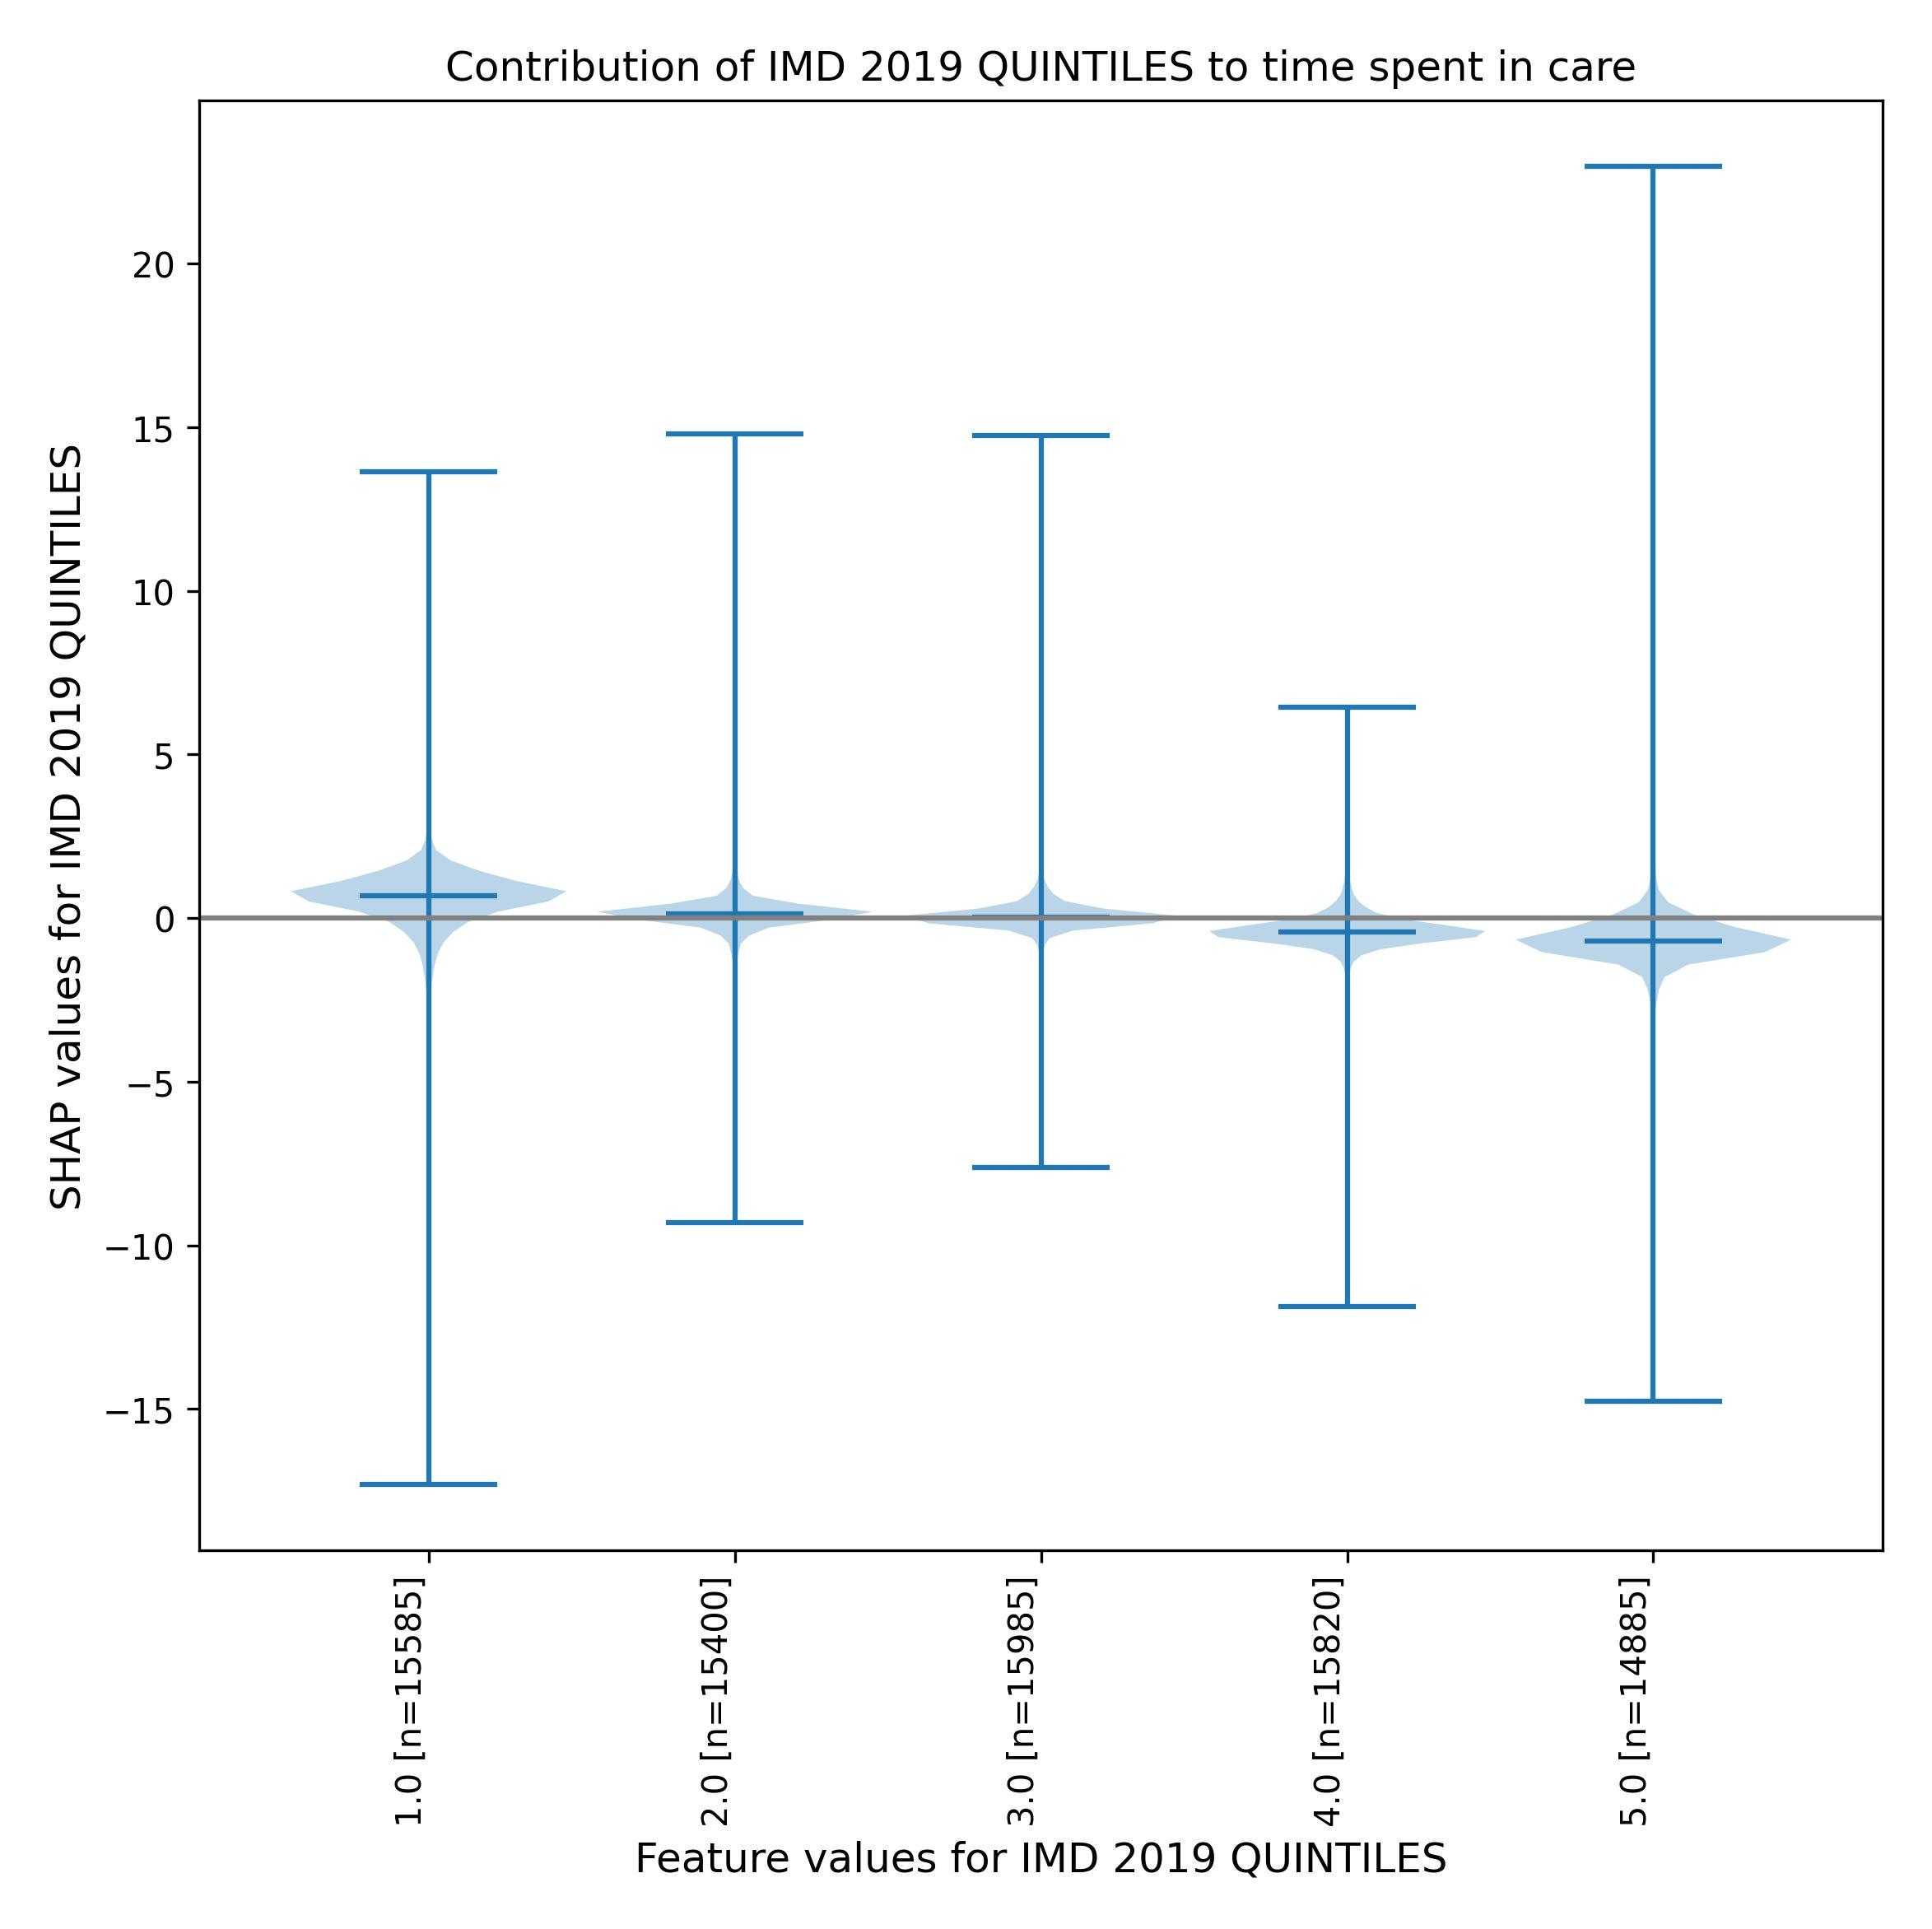
\includegraphics[width=\linewidth]{images/output_results_from_SDE/180_xgboost_in_care_exploratory_population_12_features_violin_shap_IMD_2019_QUINTILES_kfold0.jpg}
        \caption{In care}
        \label{fig:sub4}
    \end{subfigure}
    \hfill
    \begin{subfigure}[t]{0.31\textwidth}
        \centering
        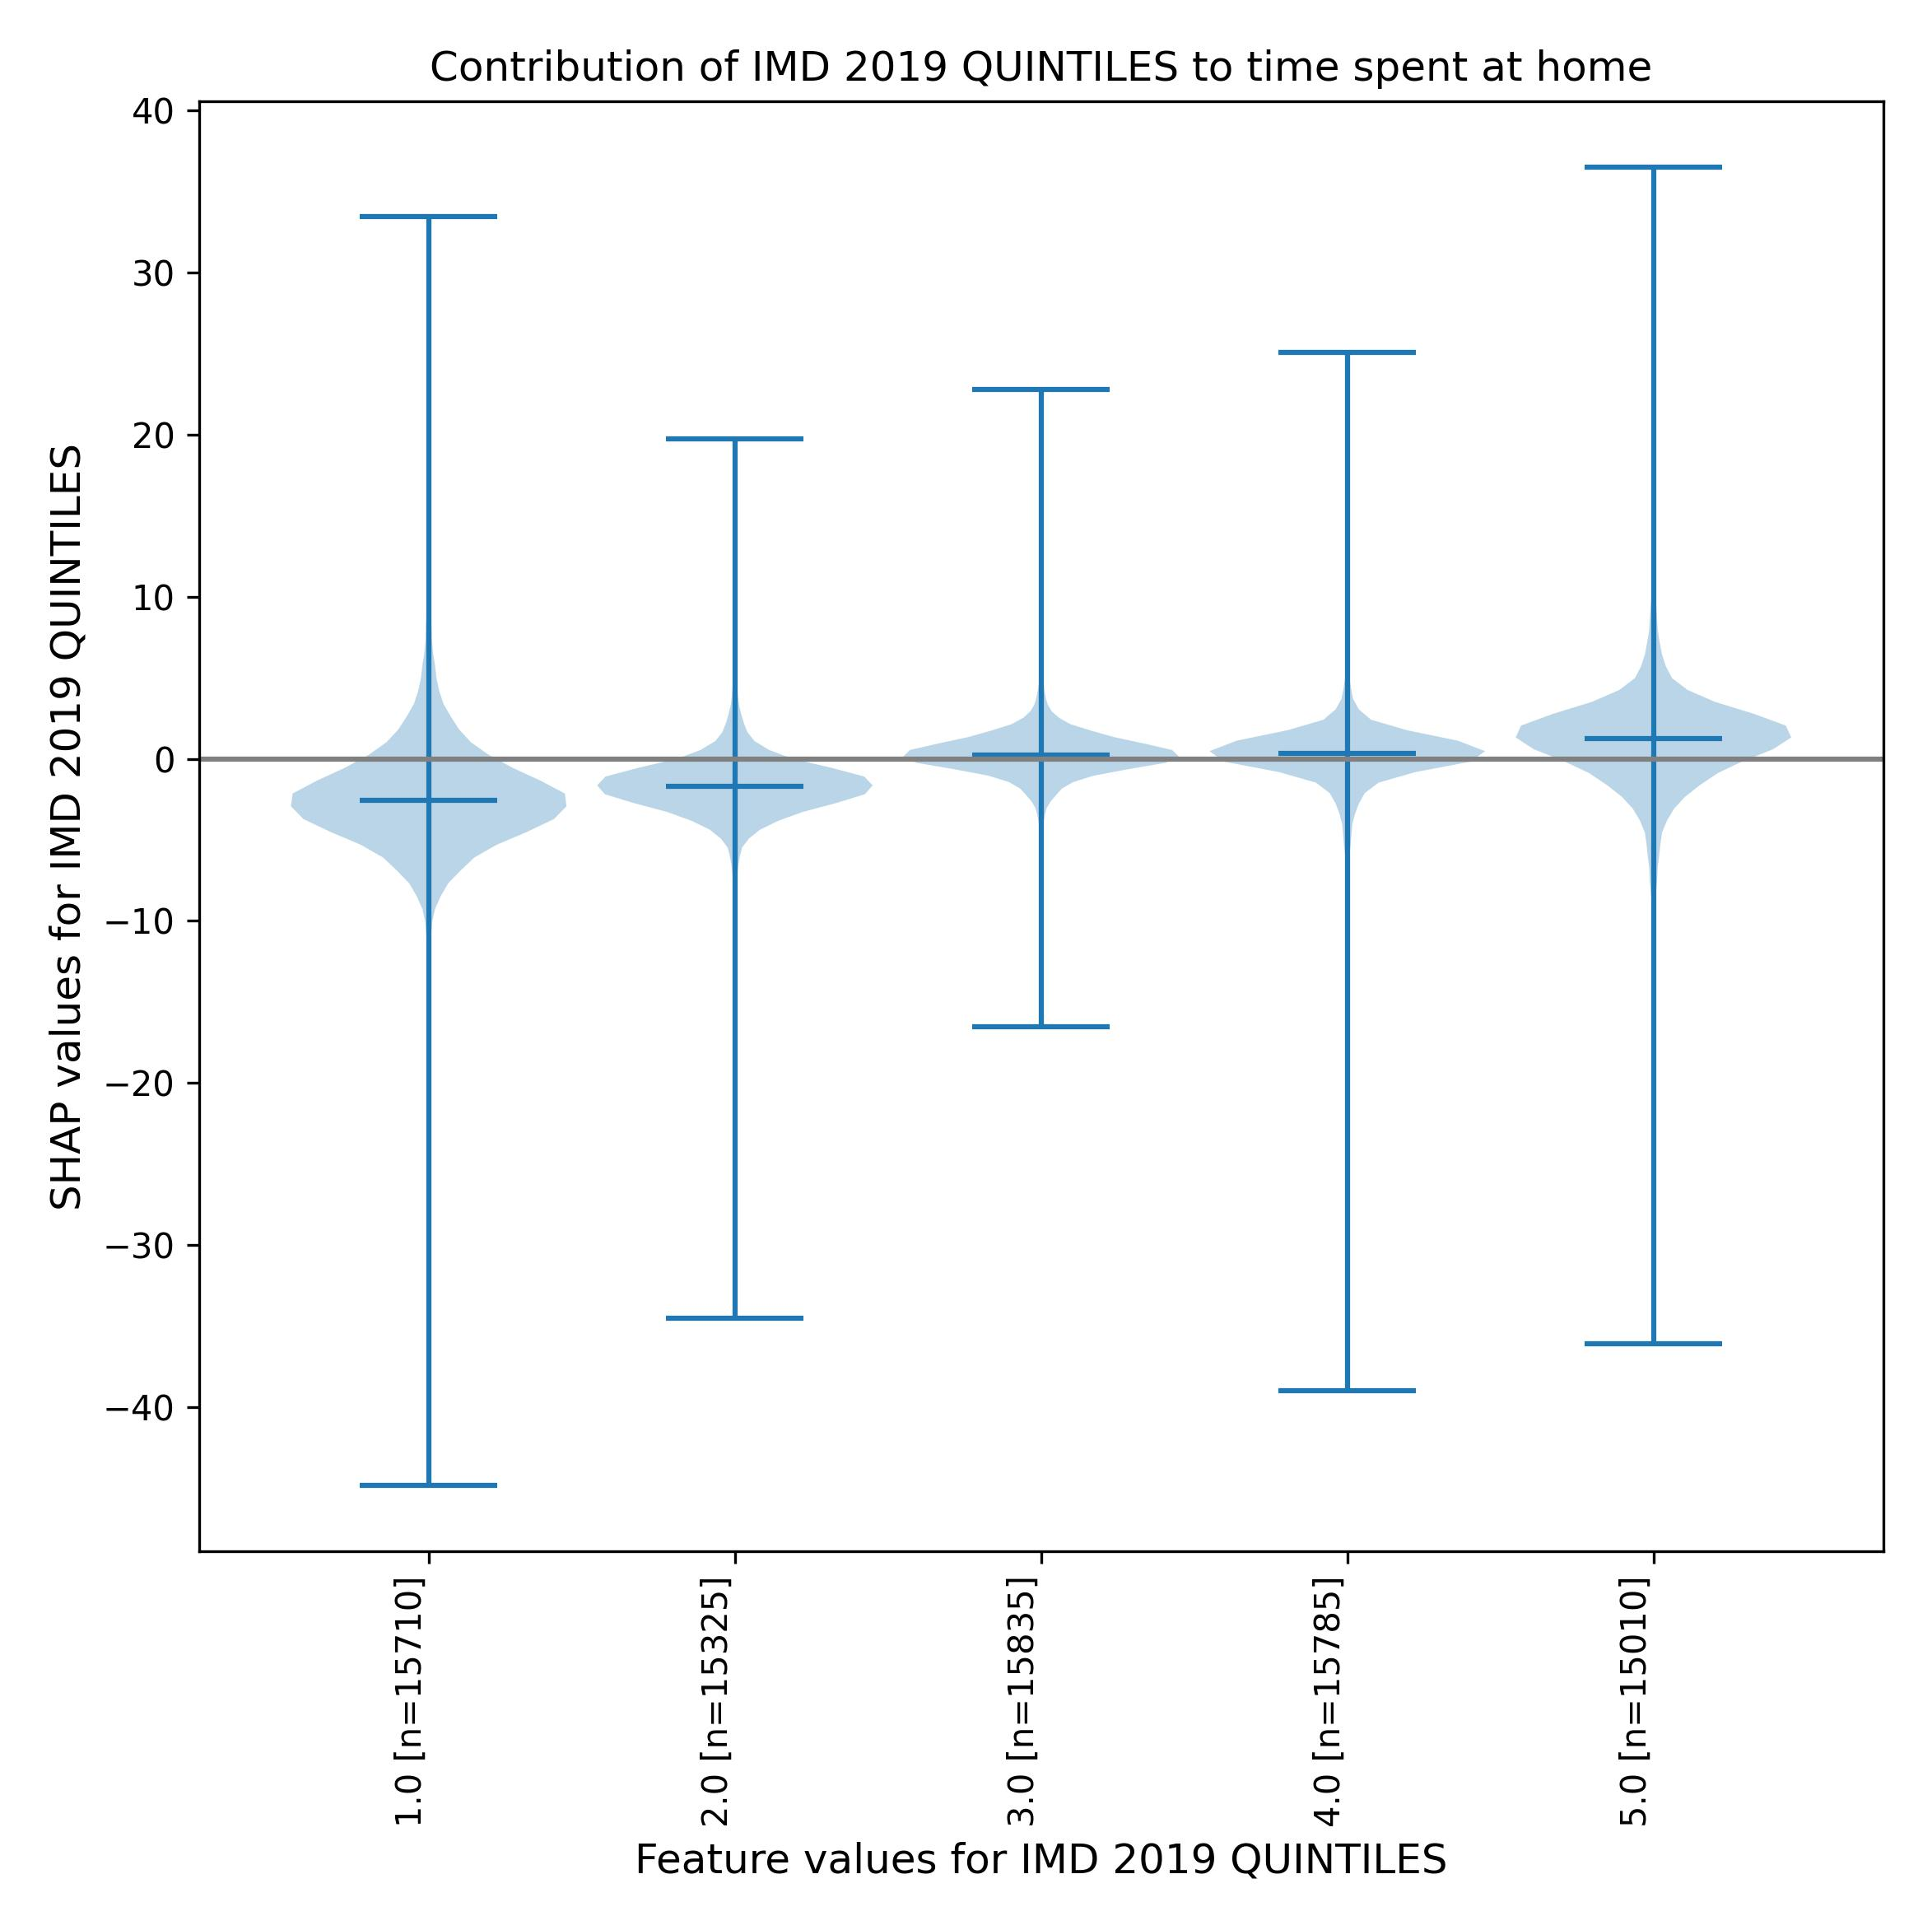
\includegraphics[width=\linewidth]{images/output_results_from_SDE/190_xgboost_at_home_exploratory_population_12_features_violin_shap_IMD_2019_QUINTILES_kfold0.jpg}
        \caption{At home}
        \label{fig:sub5}
    \end{subfigure}
    \hfill
    \begin{subfigure}[t]{0.31\textwidth}
        \centering
        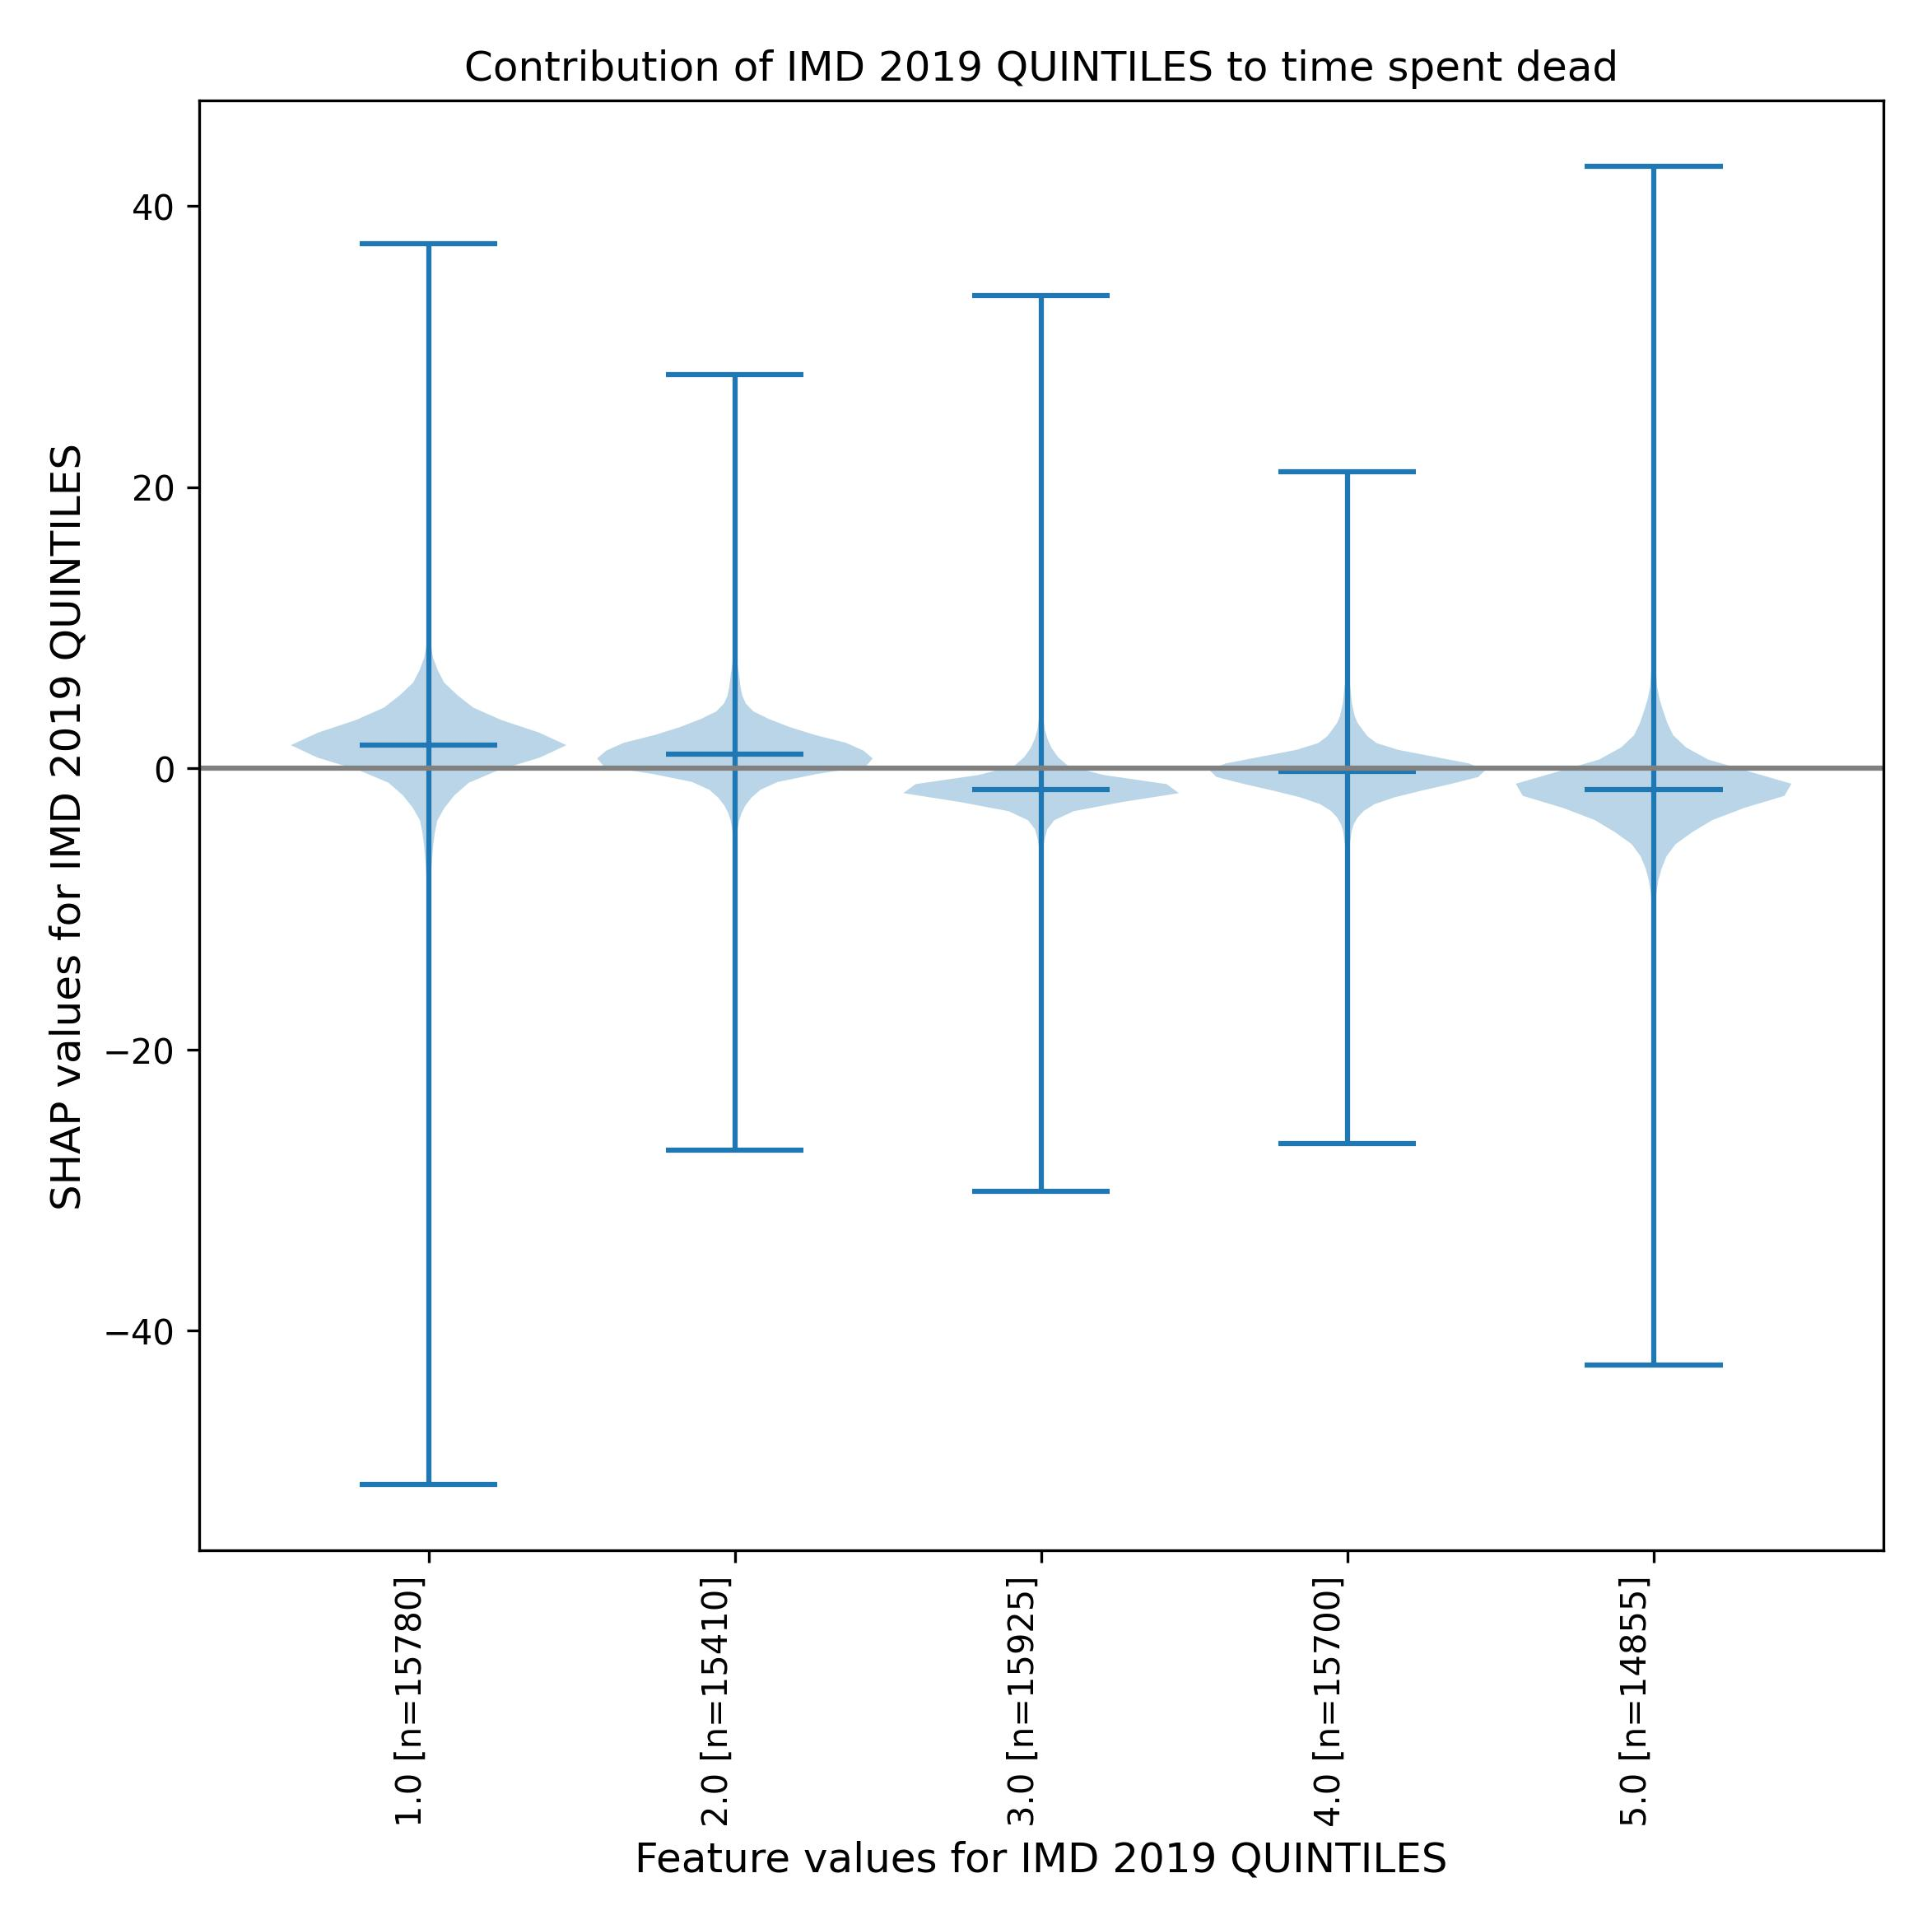
\includegraphics[width=\linewidth]{images/output_results_from_SDE/200_xgboost_dead_exploratory_population_12_features_violin_shap_IMD_2019_QUINTILES_kfold0.jpg}
        \caption{Dead}
        \label{fig:sub6}
    \end{subfigure}
    \caption*{IMD quintile}

    \vspace{2em}

    % ---------- Row 3 ----------
    \begin{subfigure}[t]{0.31\textwidth}
        \centering
        \includegraphics[width=\linewidth]{images/output_results_from_SDE/180_xgboost_in_care_exploratory_population_12_features_shap_violin_Covid status_kfold0.jpg}
        \caption{In care}
        \label{fig:sub7}
    \end{subfigure}
    \hfill
    \begin{subfigure}[t]{0.31\textwidth}
        \centering
        \includegraphics[width=\linewidth]{images/output_results_from_SDE/190_xgboost_at_home_exploratory_population_12_features_shap_violin_Covid status_kfold0.jpg}
        \caption{At home}
        \label{fig:sub8}
    \end{subfigure}
    \hfill
    \begin{subfigure}[t]{0.31\textwidth}
        \centering
        \includegraphics[width=\linewidth]{images/output_results_from_SDE/200_xgboost_dead_exploratory_population_12_features_shap_violin_Covid status_kfold0.jpg}
        \caption{Dead}
        \label{fig:sub9}
    \end{subfigure}
    \caption*{Covid status}

    \vspace{2em}

    \caption{SHAP analysis on how feature values influence XGBoost model predictions for time spent in a) NHS inpatient care (left), b) at home (alive, and outside of NHS inpatient care), and c) dead, in the year after stroke. Features shown are ethnicity (top), IMD quintile (1 = highest deprivation, middle), and Covid status (bottom). SHAP values are calculated for each prediction, taking into account interactions with other features. The resulting distributions for any given feature value are shown in the figure as violin plots with median and range bars.}
    \label{fig:shap_2}
\end{figure}

%%%%%%%%%%%%%%%%%%%%%%%%%%%%%%%%%%%%%%%%%%%%%%%%%%%%%%%%%%%%%%%%%%%%

\begin{figure}[htbp]
    \centering

    % ---------- Row 1 ----------
    
    \begin{subfigure}[t]{0.31\textwidth}
        \centering
        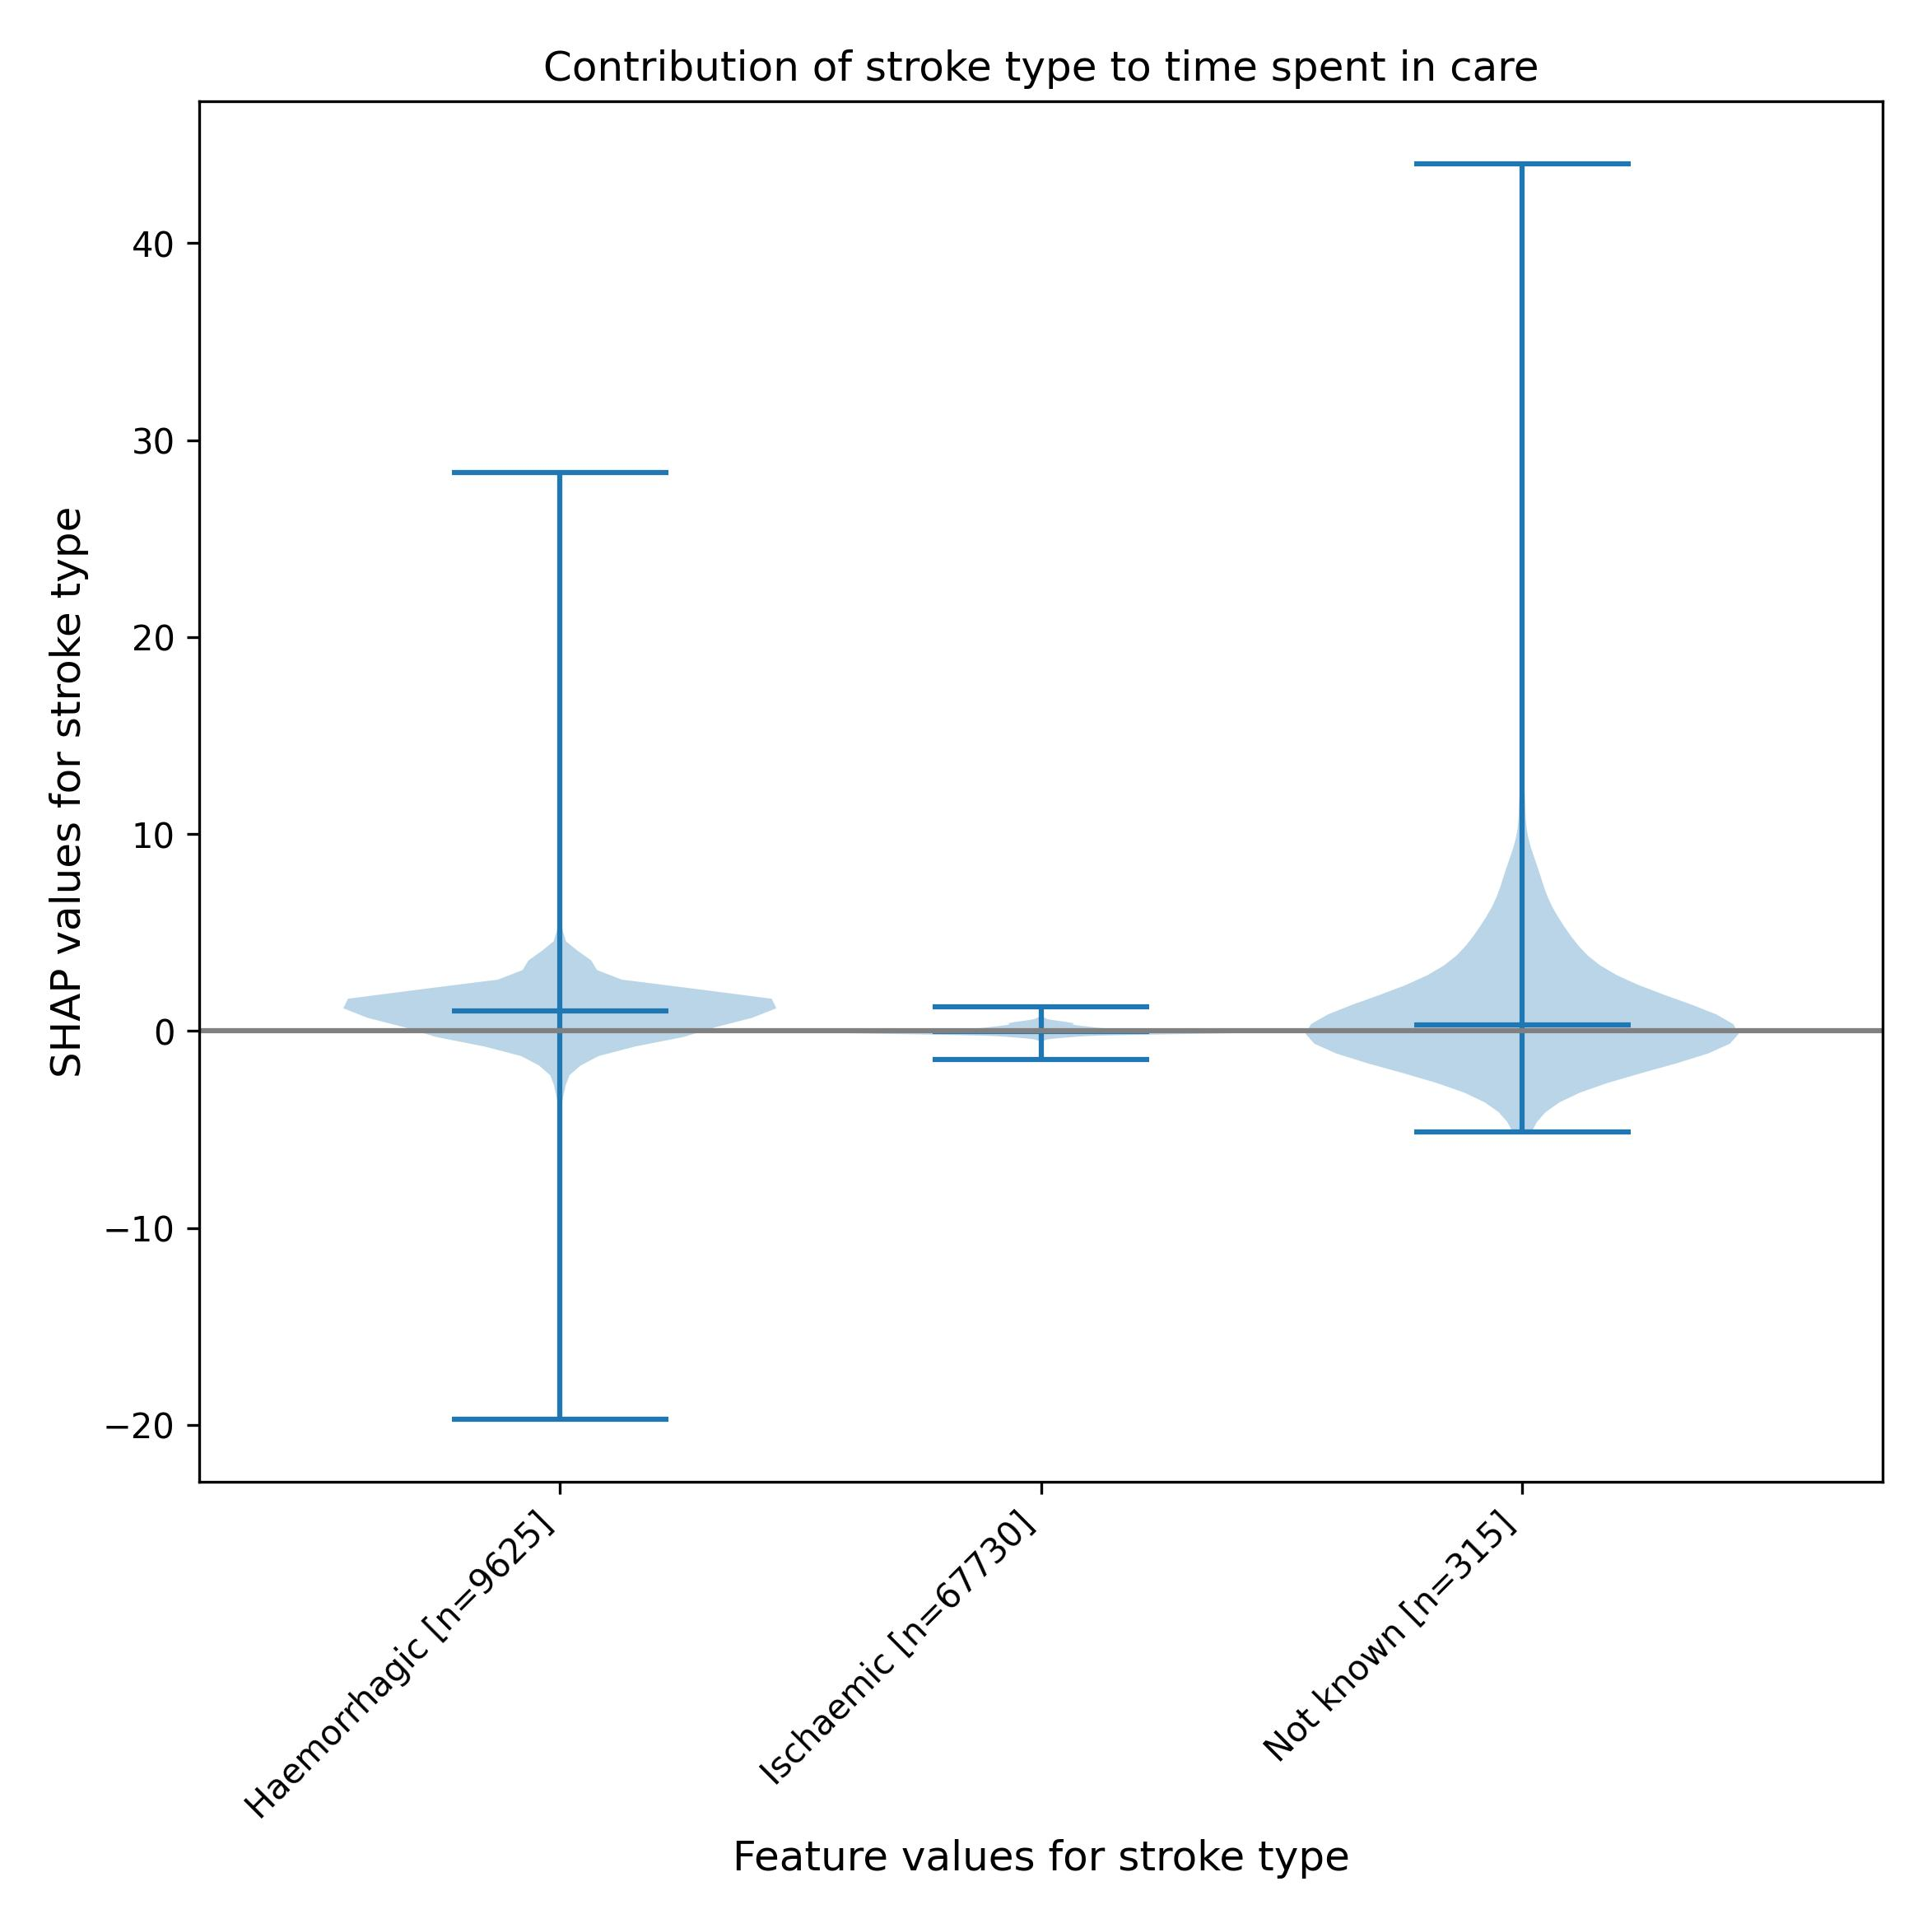
\includegraphics[width=\linewidth]{images/output_results_from_SDE/180_xgboost_in_care_exploratory_population_12_features_shap_violin_stroke type_kfold0.jpg}
        \caption{In care}
        \label{fig:sub1}
    \end{subfigure}
    \hfill
    \begin{subfigure}[t]{0.31\textwidth}
        \centering
        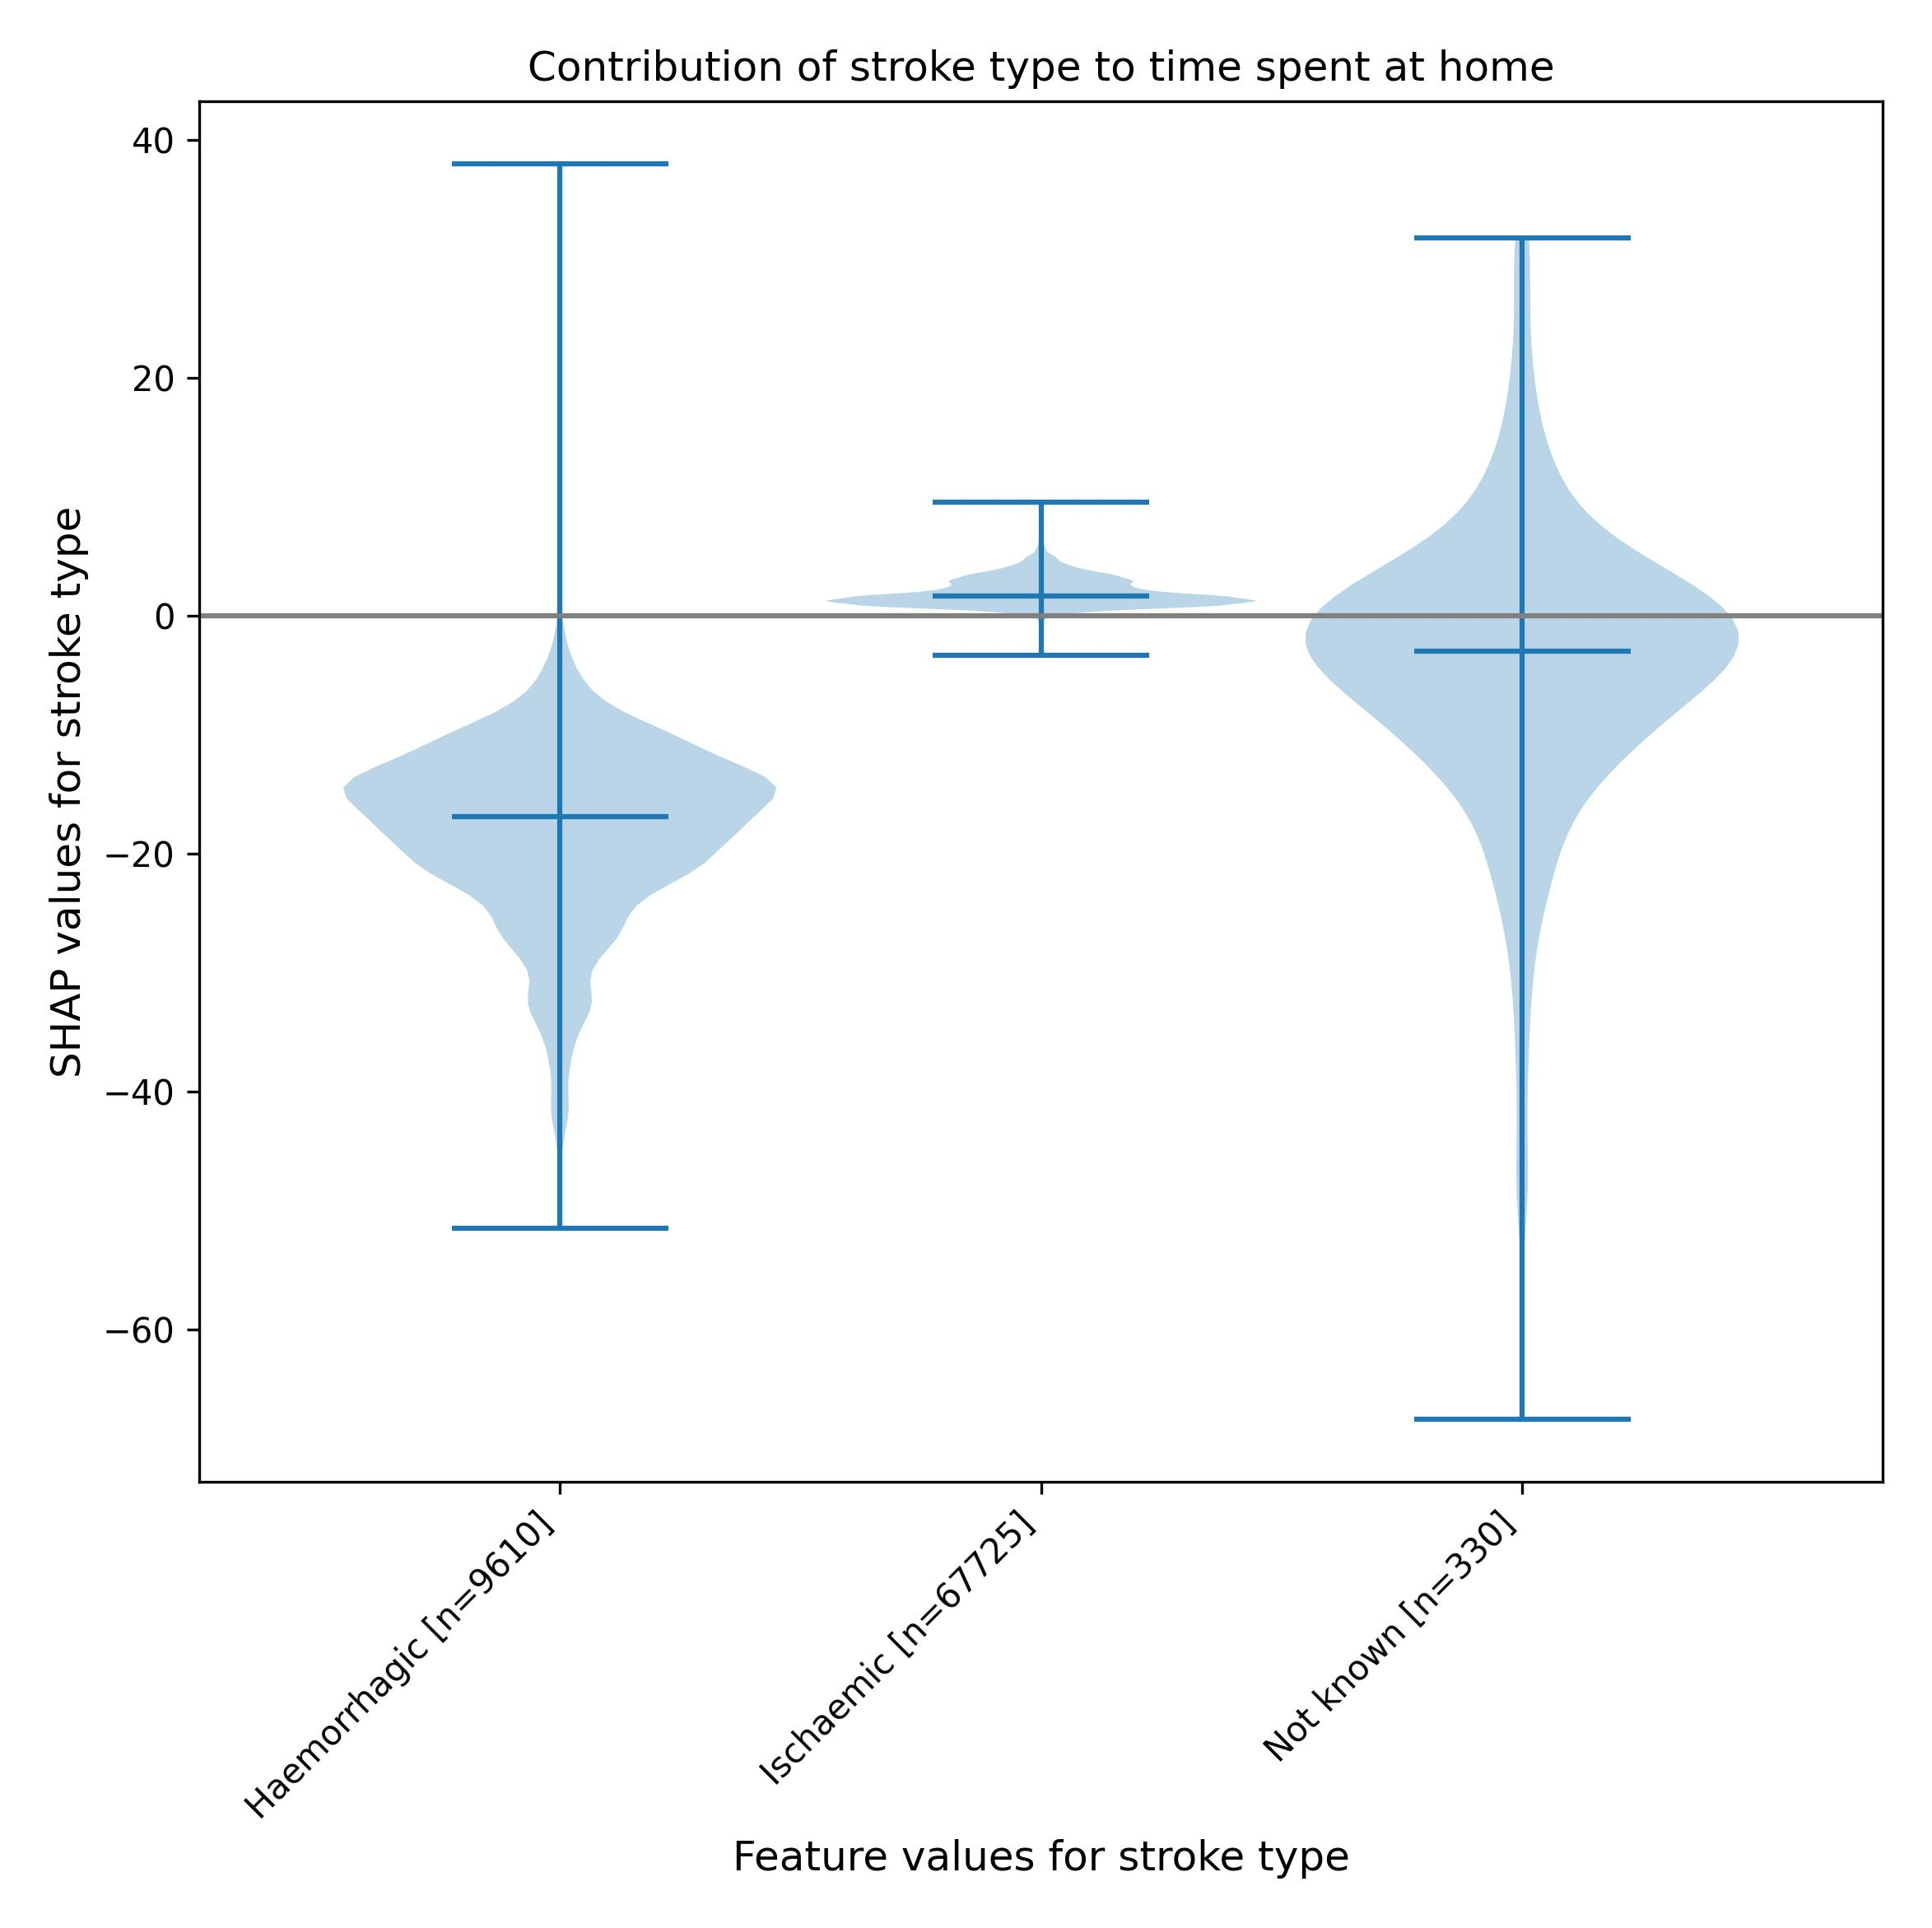
\includegraphics[width=\linewidth]{images/output_results_from_SDE/190_xgboost_at_home_exploratory_population_12_features_shap_violin_stroke type_kfold0.jpg}
        \caption{At home}
        \label{fig:sub2}
    \end{subfigure}
    \hfill
    \begin{subfigure}[t]{0.31\textwidth}
        \centering
        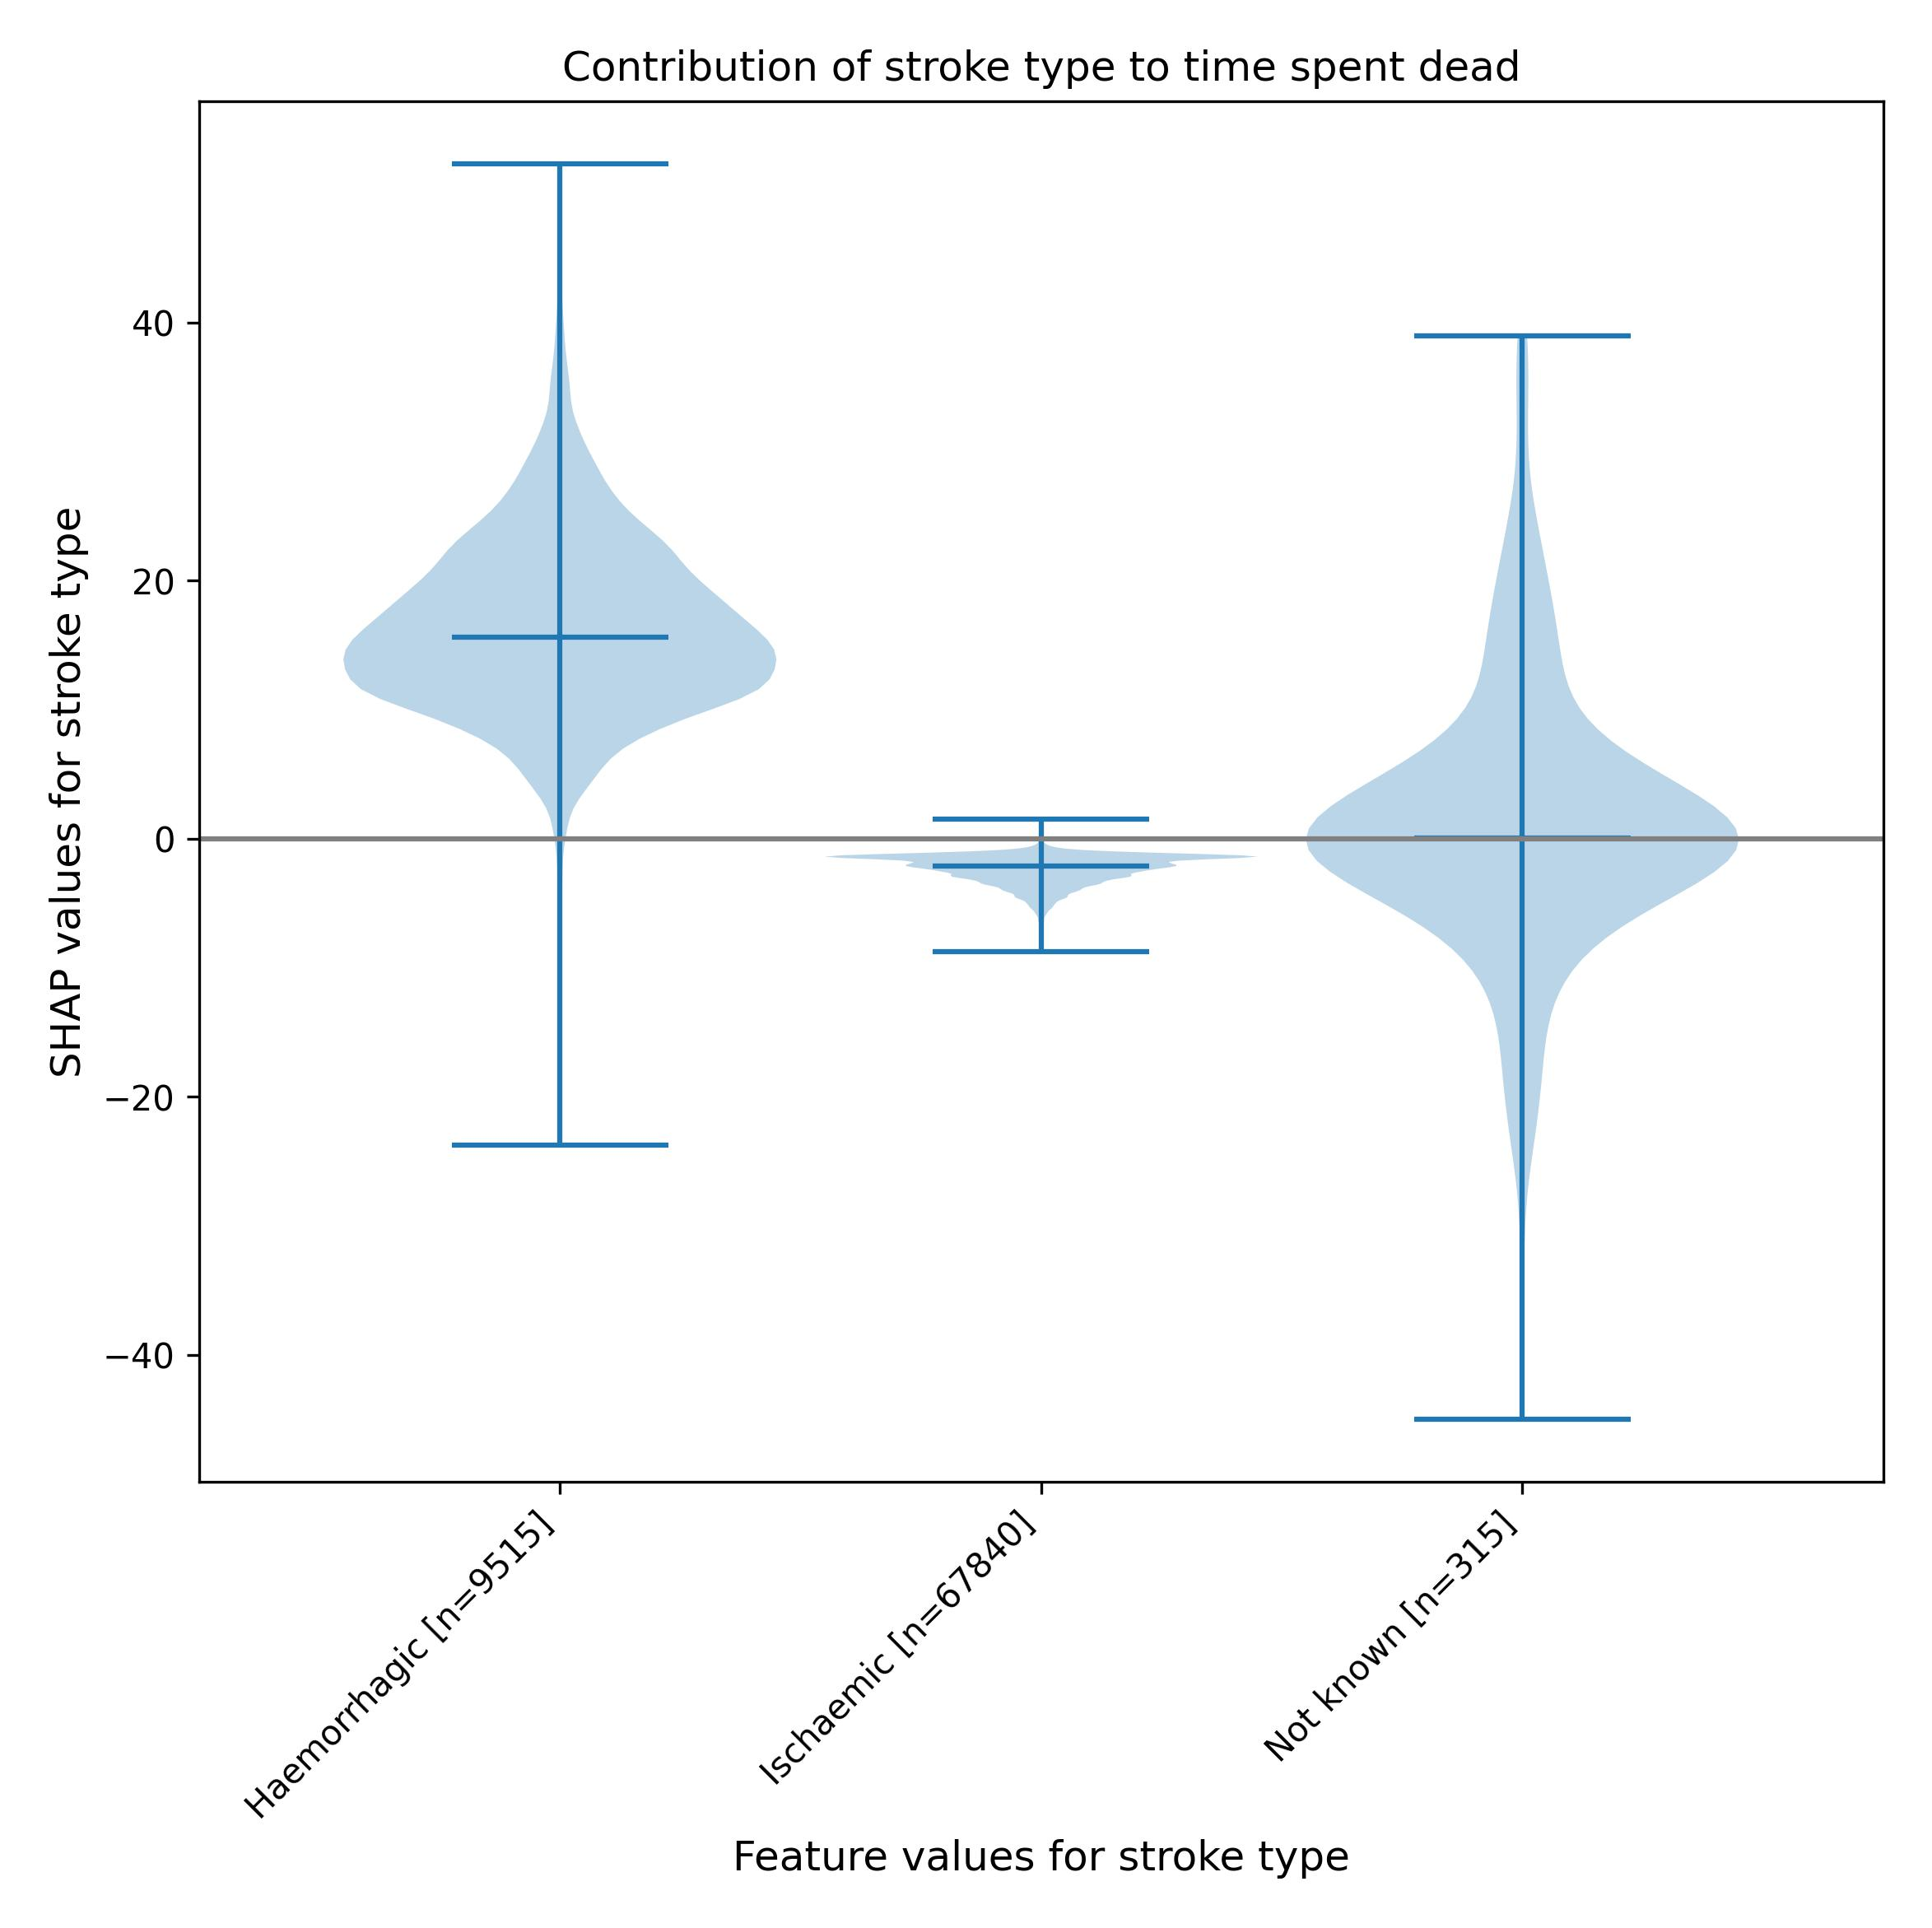
\includegraphics[width=\linewidth]{images/output_results_from_SDE/200_xgboost_dead_exploratory_population_12_features_shap_violin_stroke type_kfold0.jpg}
        \caption{Dead}
        \label{fig:sub3}
    \end{subfigure}
    \caption*{Stroke type}

    \vspace{2em} % space between rows

    % ---------- Row 2 ----------
    \begin{subfigure}[t]{0.31\textwidth}
        \centering
        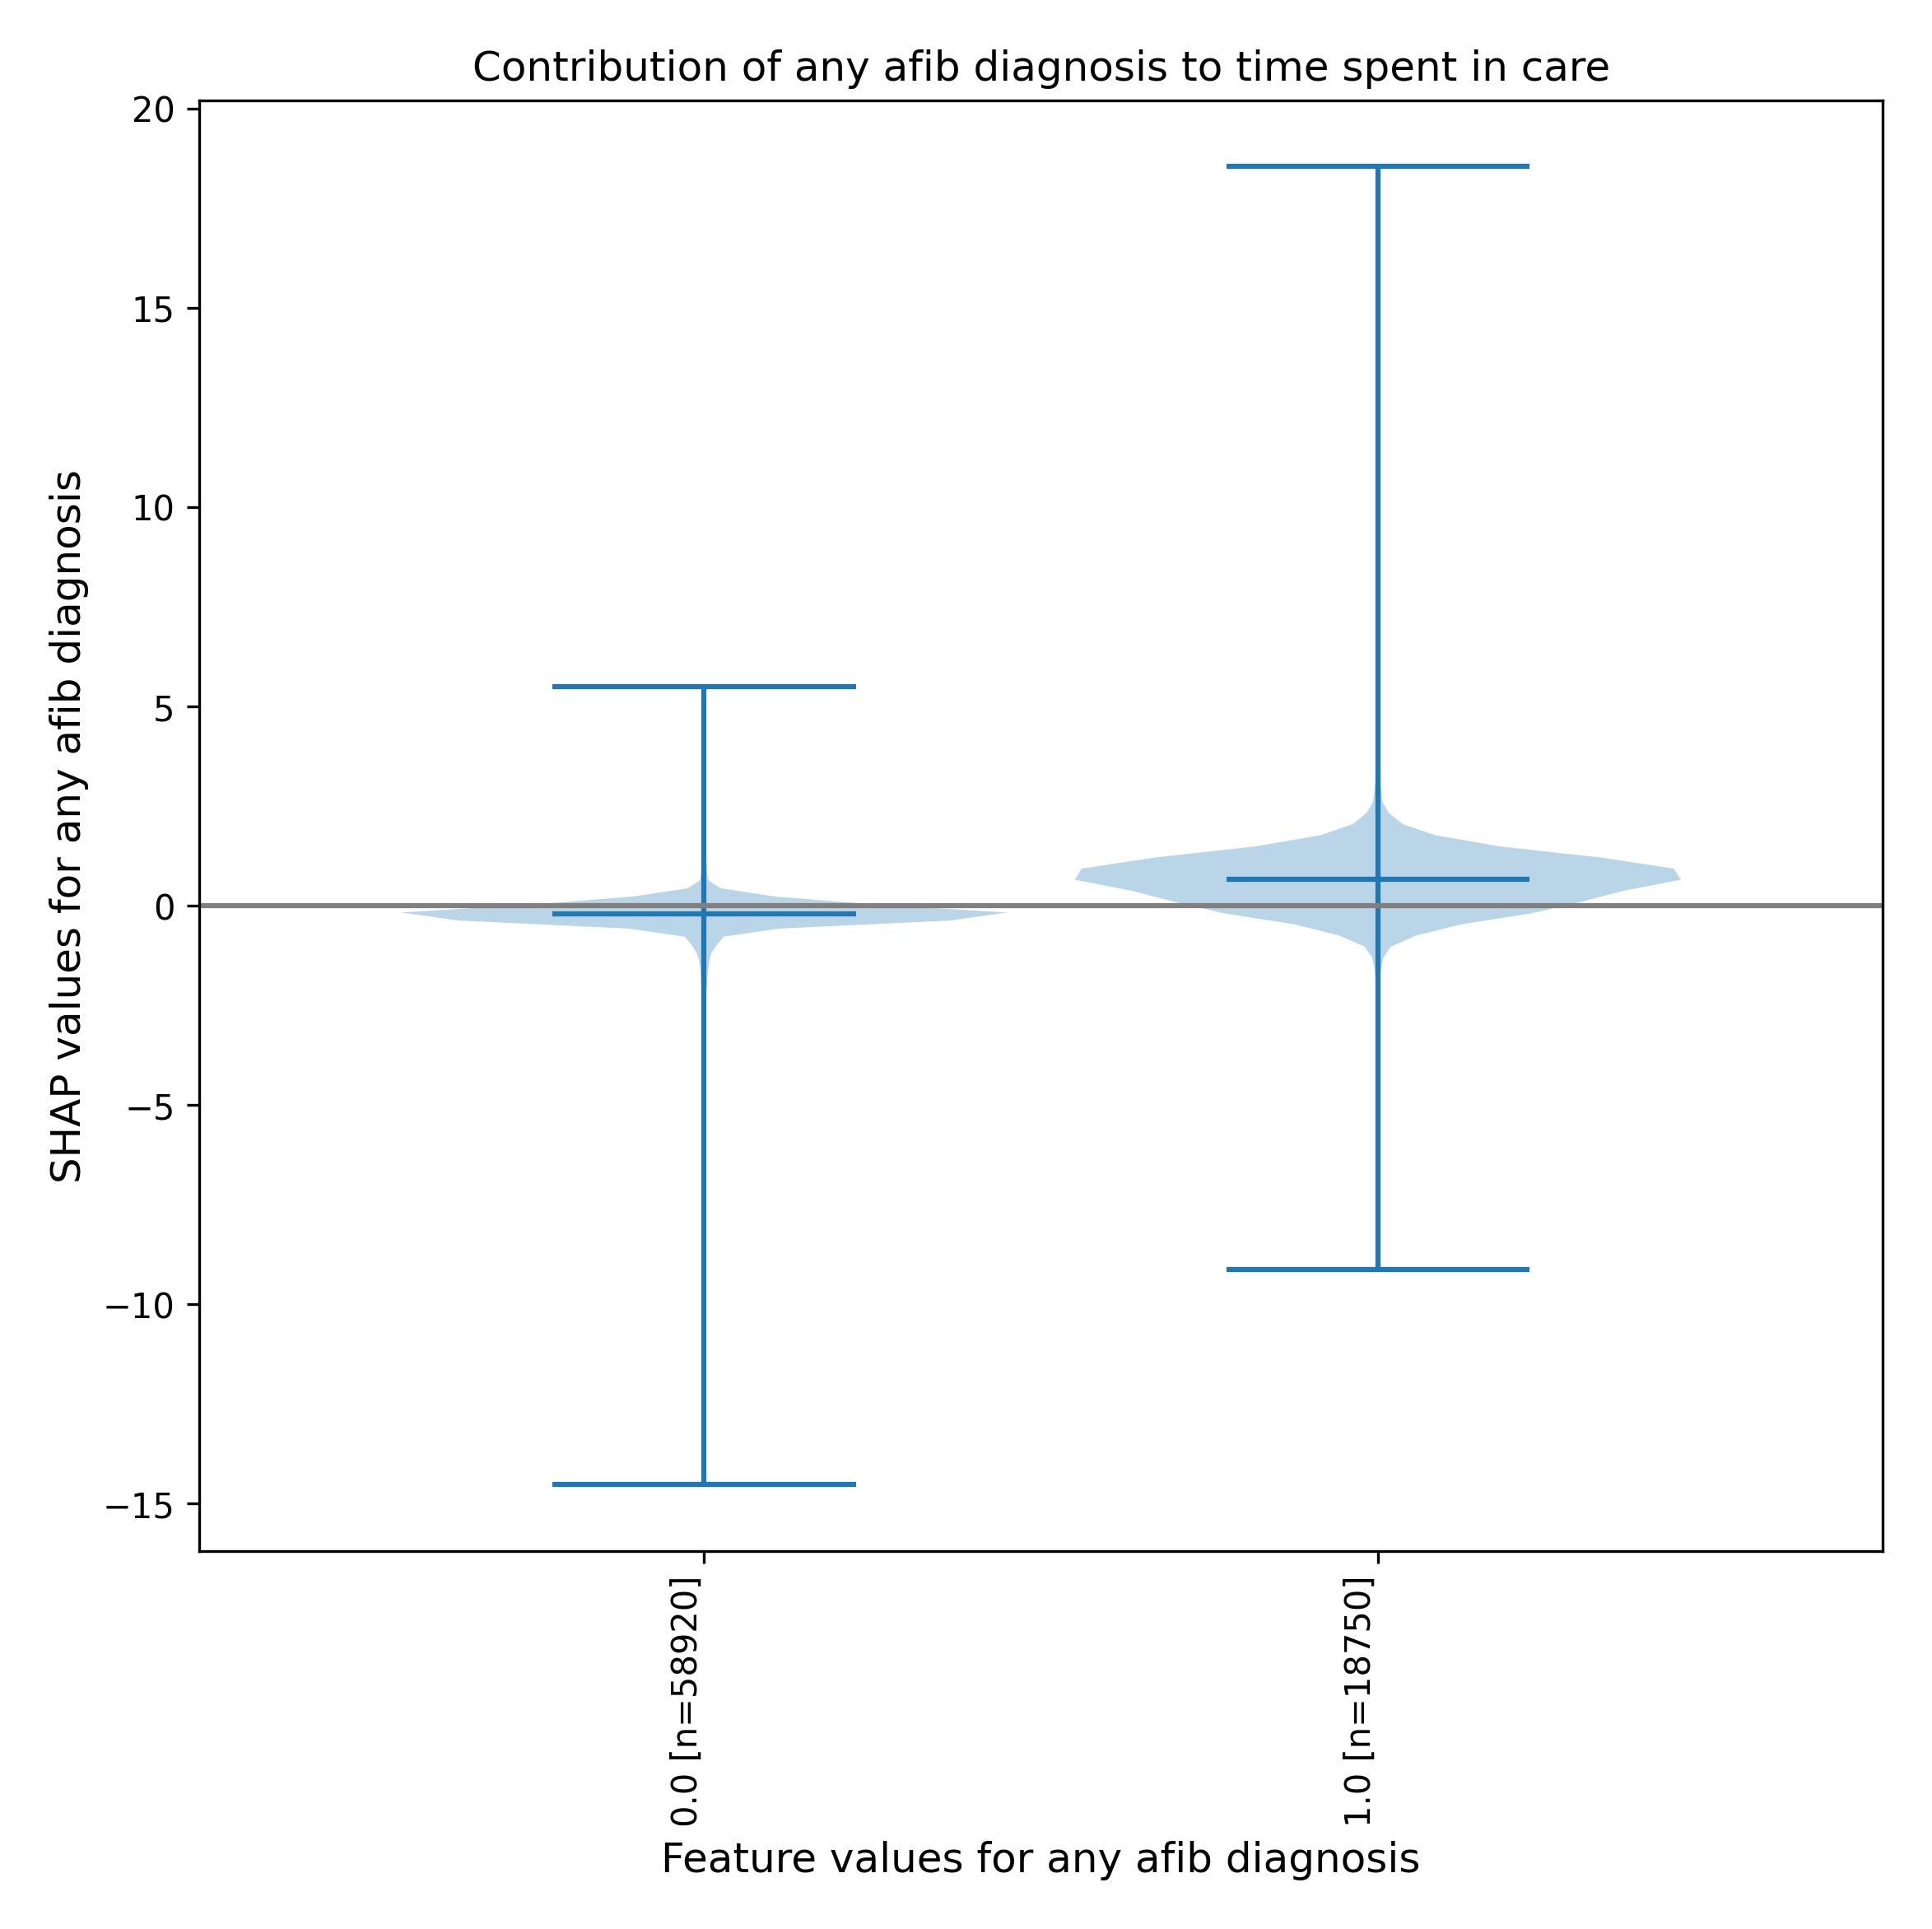
\includegraphics[width=\linewidth]{images/output_results_from_SDE/180_xgboost_in_care_exploratory_population_12_features_violin_shap_any_afib_diagnosis_kfold0.jpg}
        \caption{In care}
        \label{fig:sub4}
    \end{subfigure}
    \hfill
    \begin{subfigure}[t]{0.31\textwidth}
        \centering
        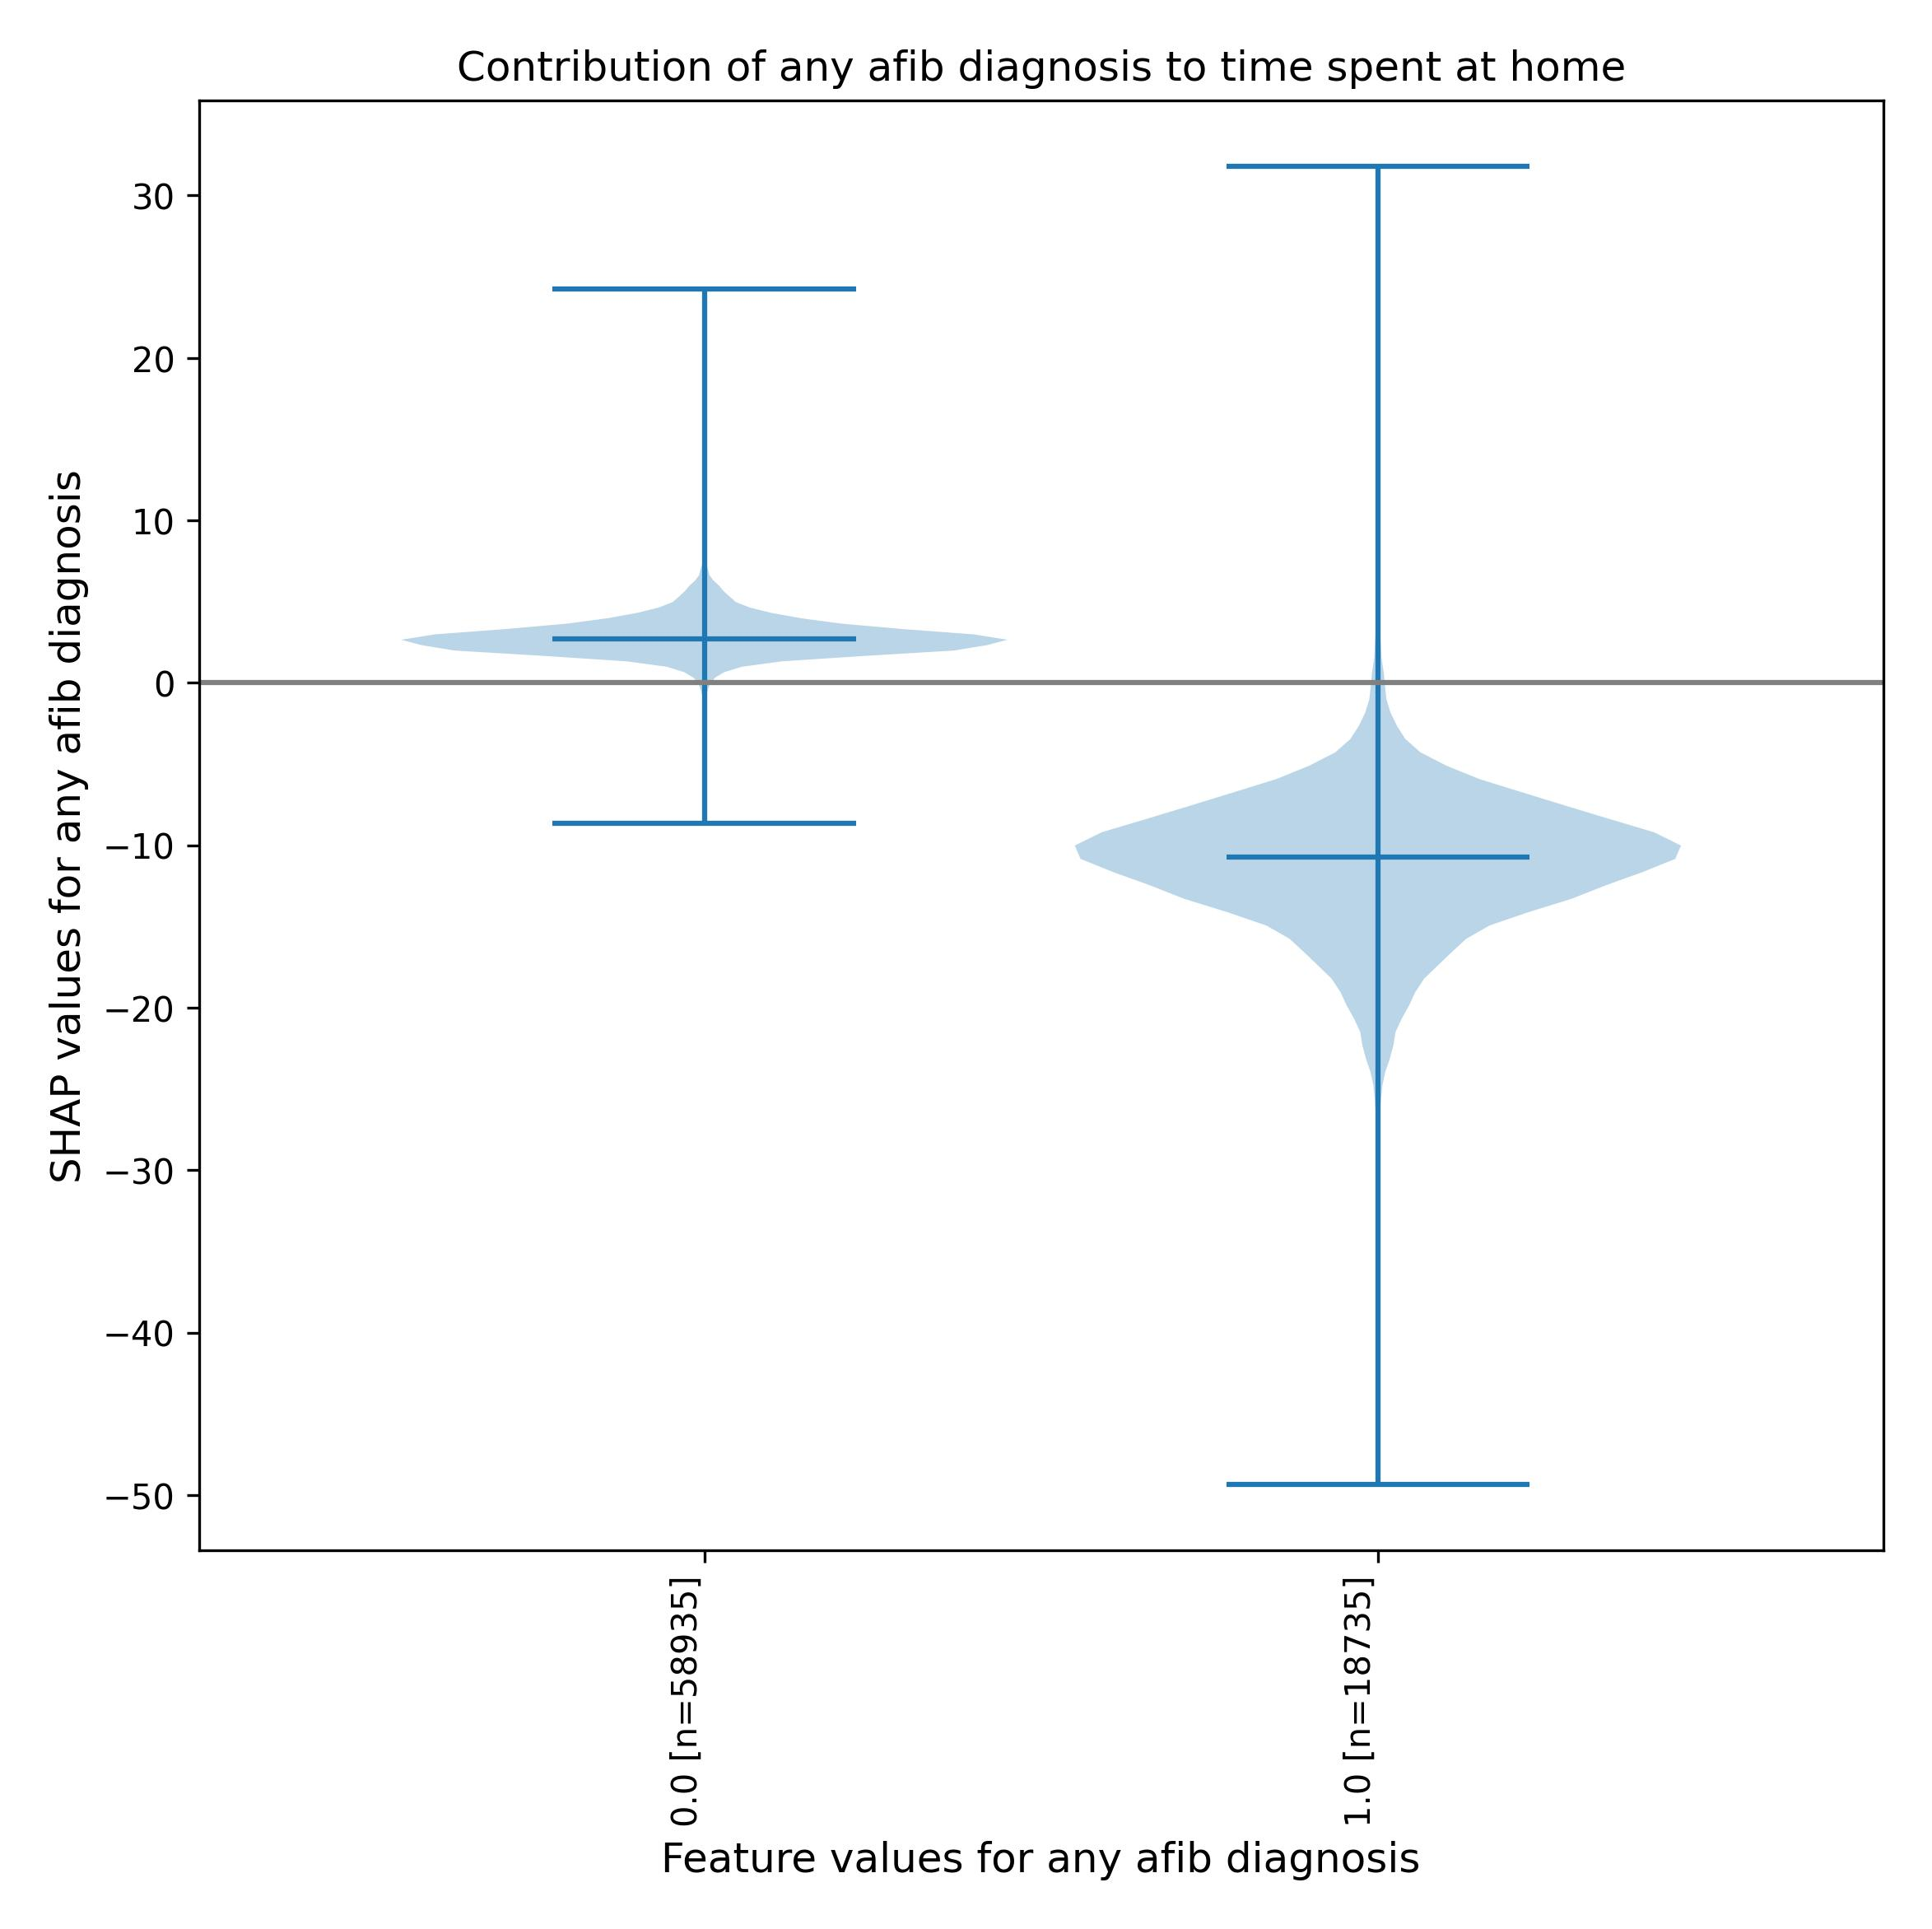
\includegraphics[width=\linewidth]{images/output_results_from_SDE/190_xgboost_at_home_exploratory_population_12_features_violin_shap_any_afib_diagnosis_kfold0.jpg}
        \caption{At home}
        \label{fig:sub5}
    \end{subfigure}
    \hfill
    \begin{subfigure}[t]{0.31\textwidth}
        \centering
        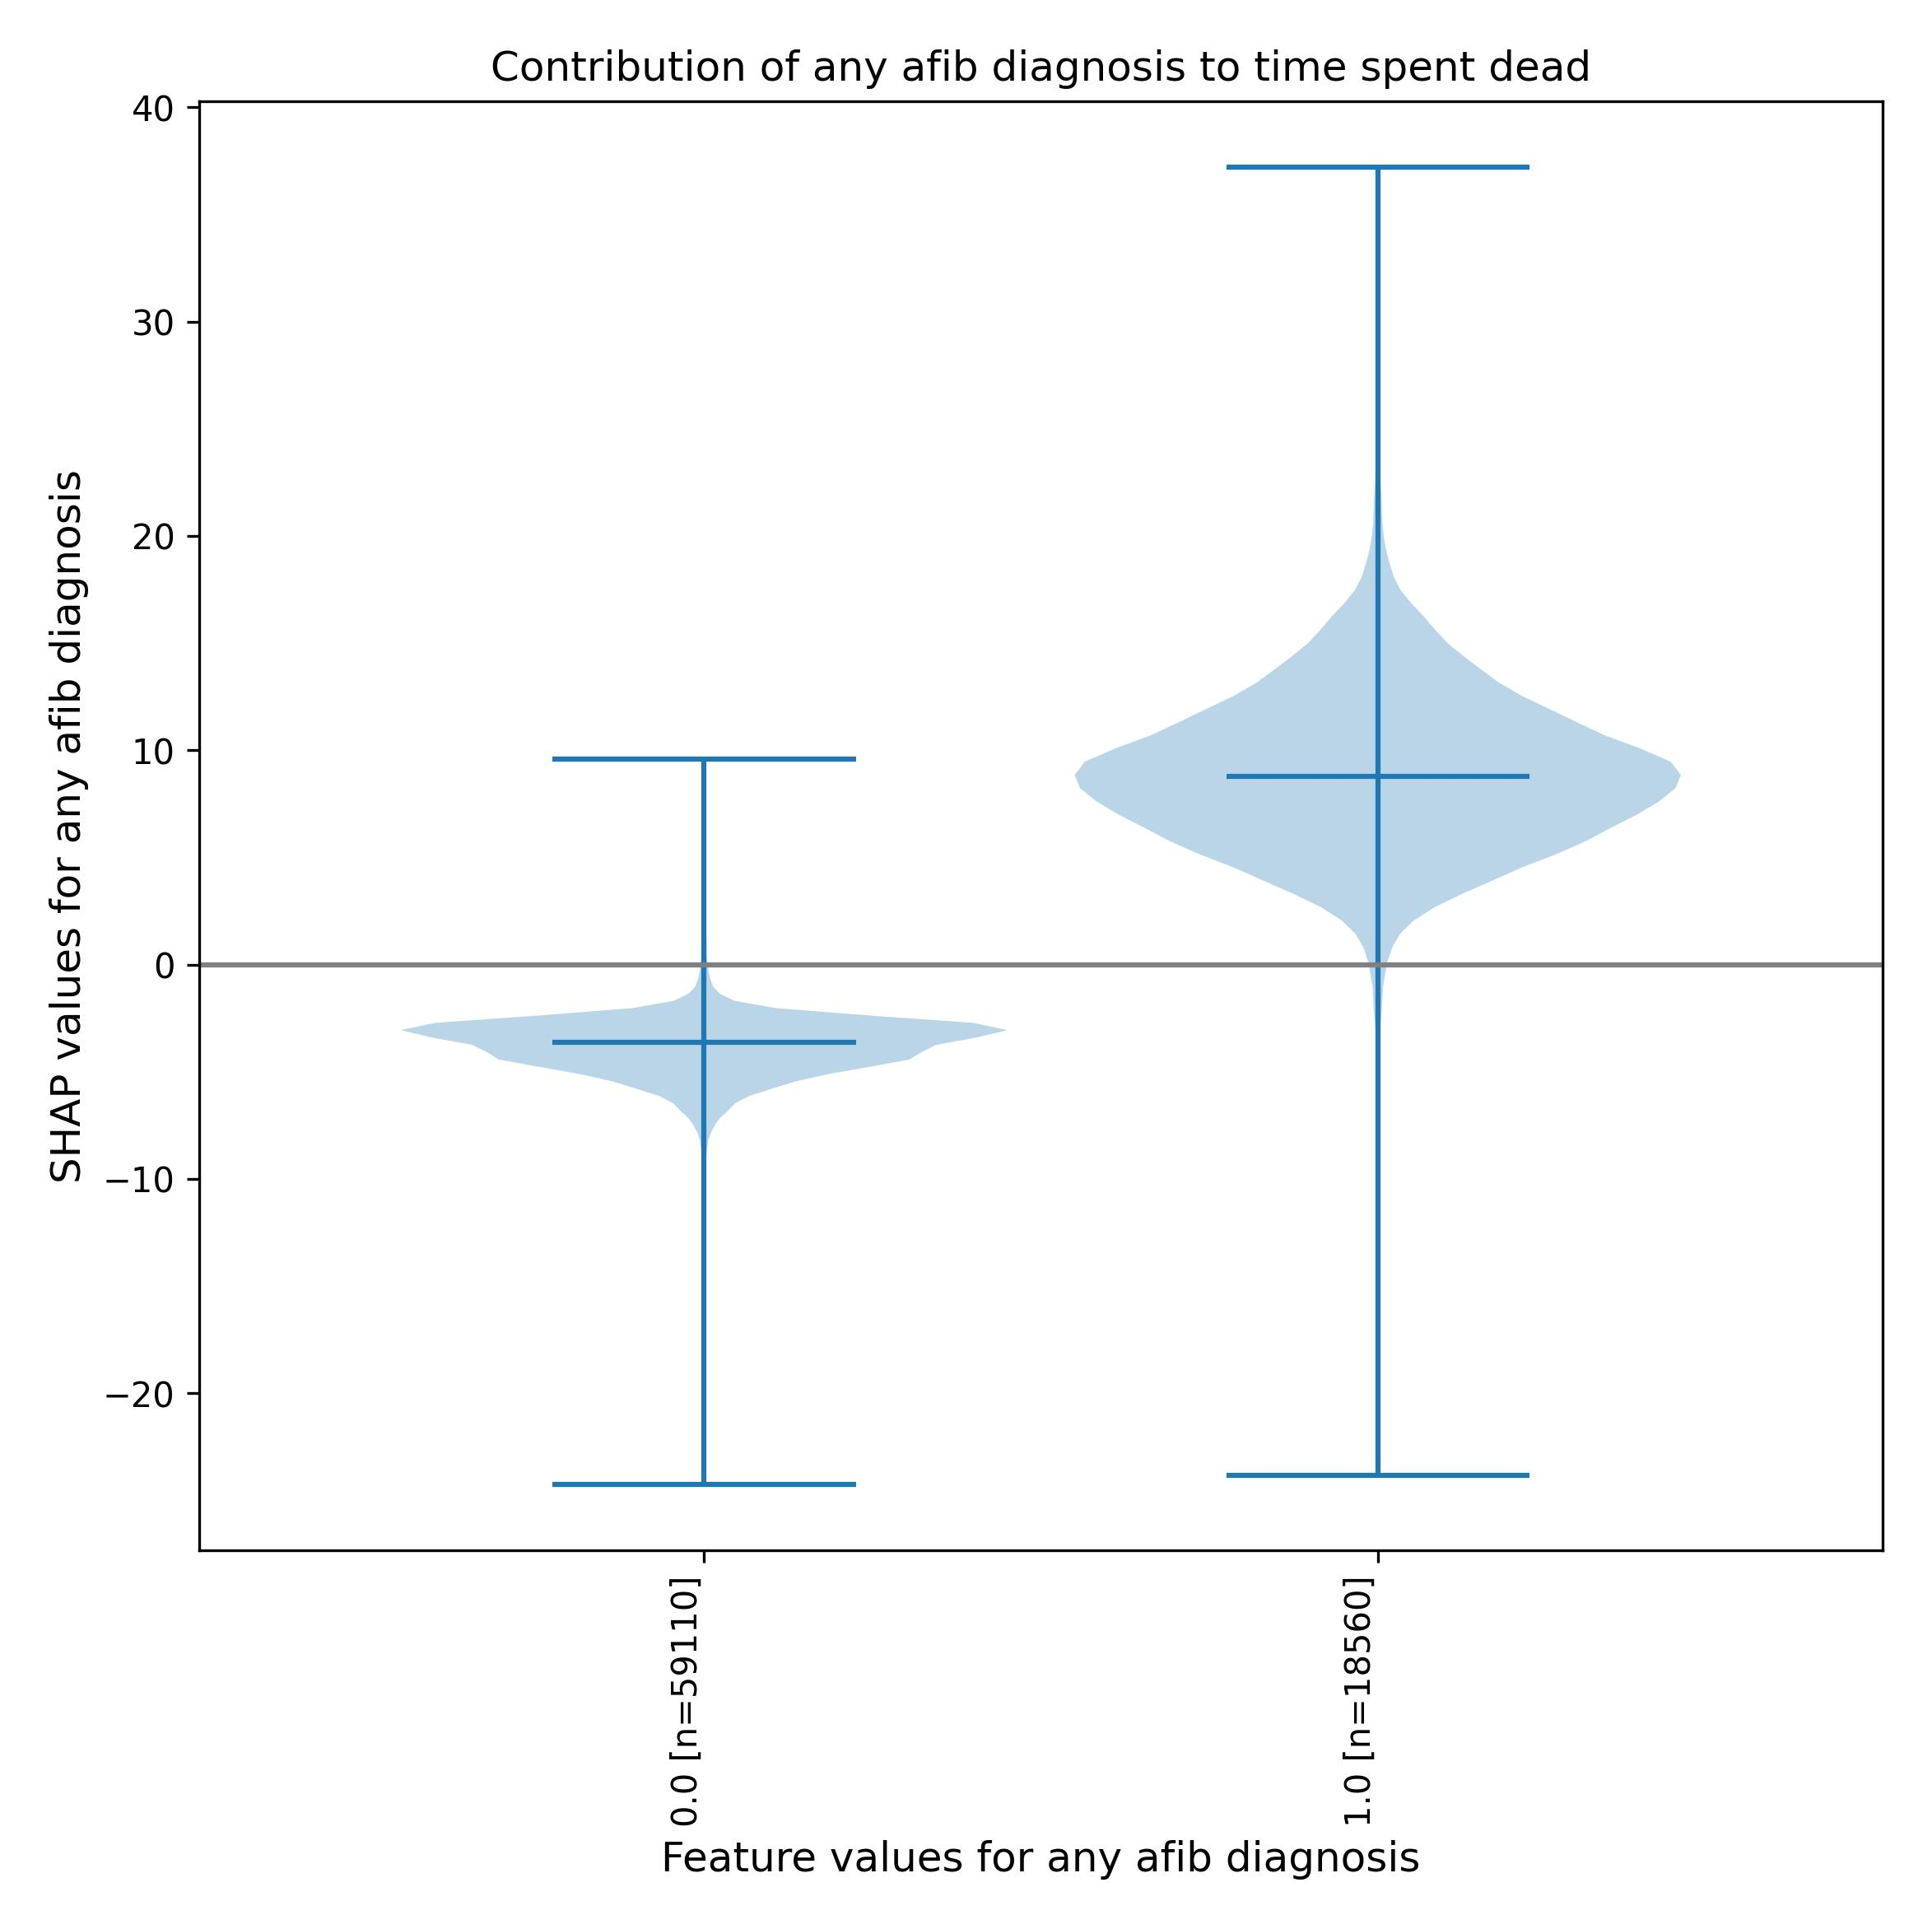
\includegraphics[width=\linewidth]{images/output_results_from_SDE/200_xgboost_dead_exploratory_population_12_features_violin_shap_any_afib_diagnosis_kfold0.jpg}
        \caption{Dead}
        \label{fig:sub6}
    \end{subfigure}
    \caption*{Atrial fibrillation}

    \vspace{2em}

    % ---------- Row 3 ----------
    \begin{subfigure}[t]{0.31\textwidth}
        \centering
        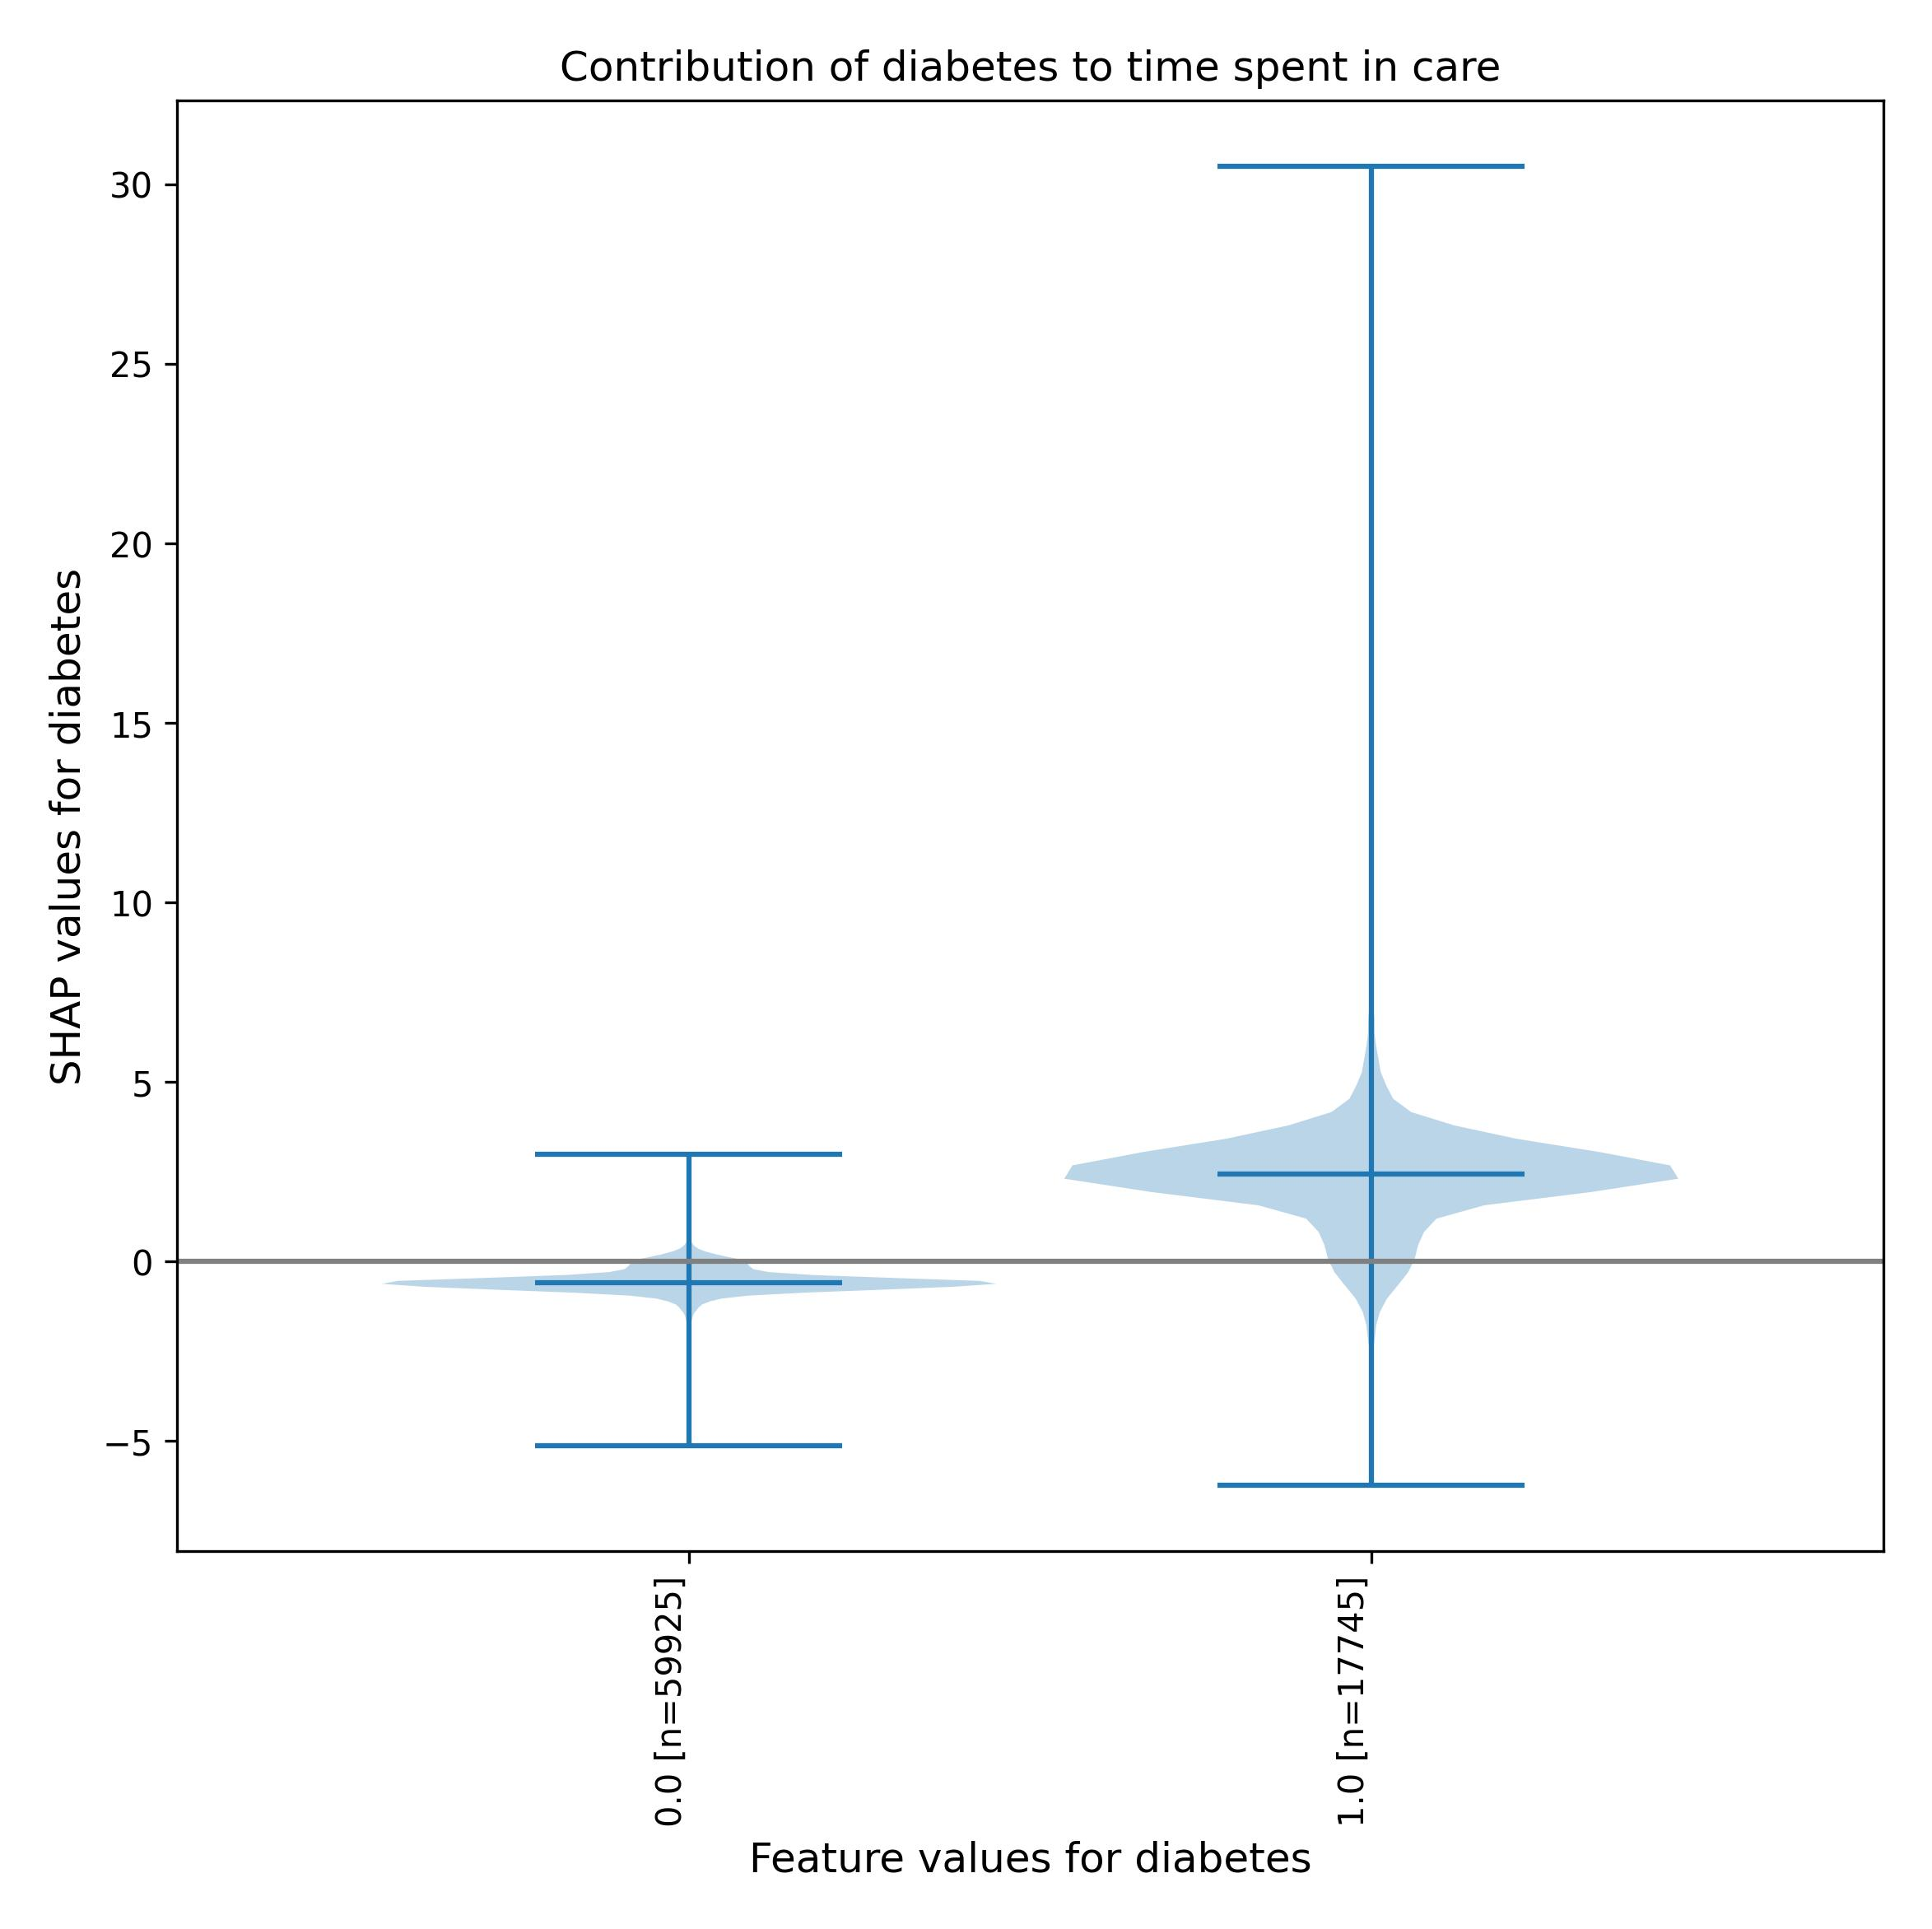
\includegraphics[width=\linewidth]{images/output_results_from_SDE/180_xgboost_in_care_exploratory_population_12_features_violin_shap_diabetes_kfold0.jpg}
        \caption{In care}
        \label{fig:sub7}
    \end{subfigure}
    \hfill
    \begin{subfigure}[t]{0.31\textwidth}
        \centering
        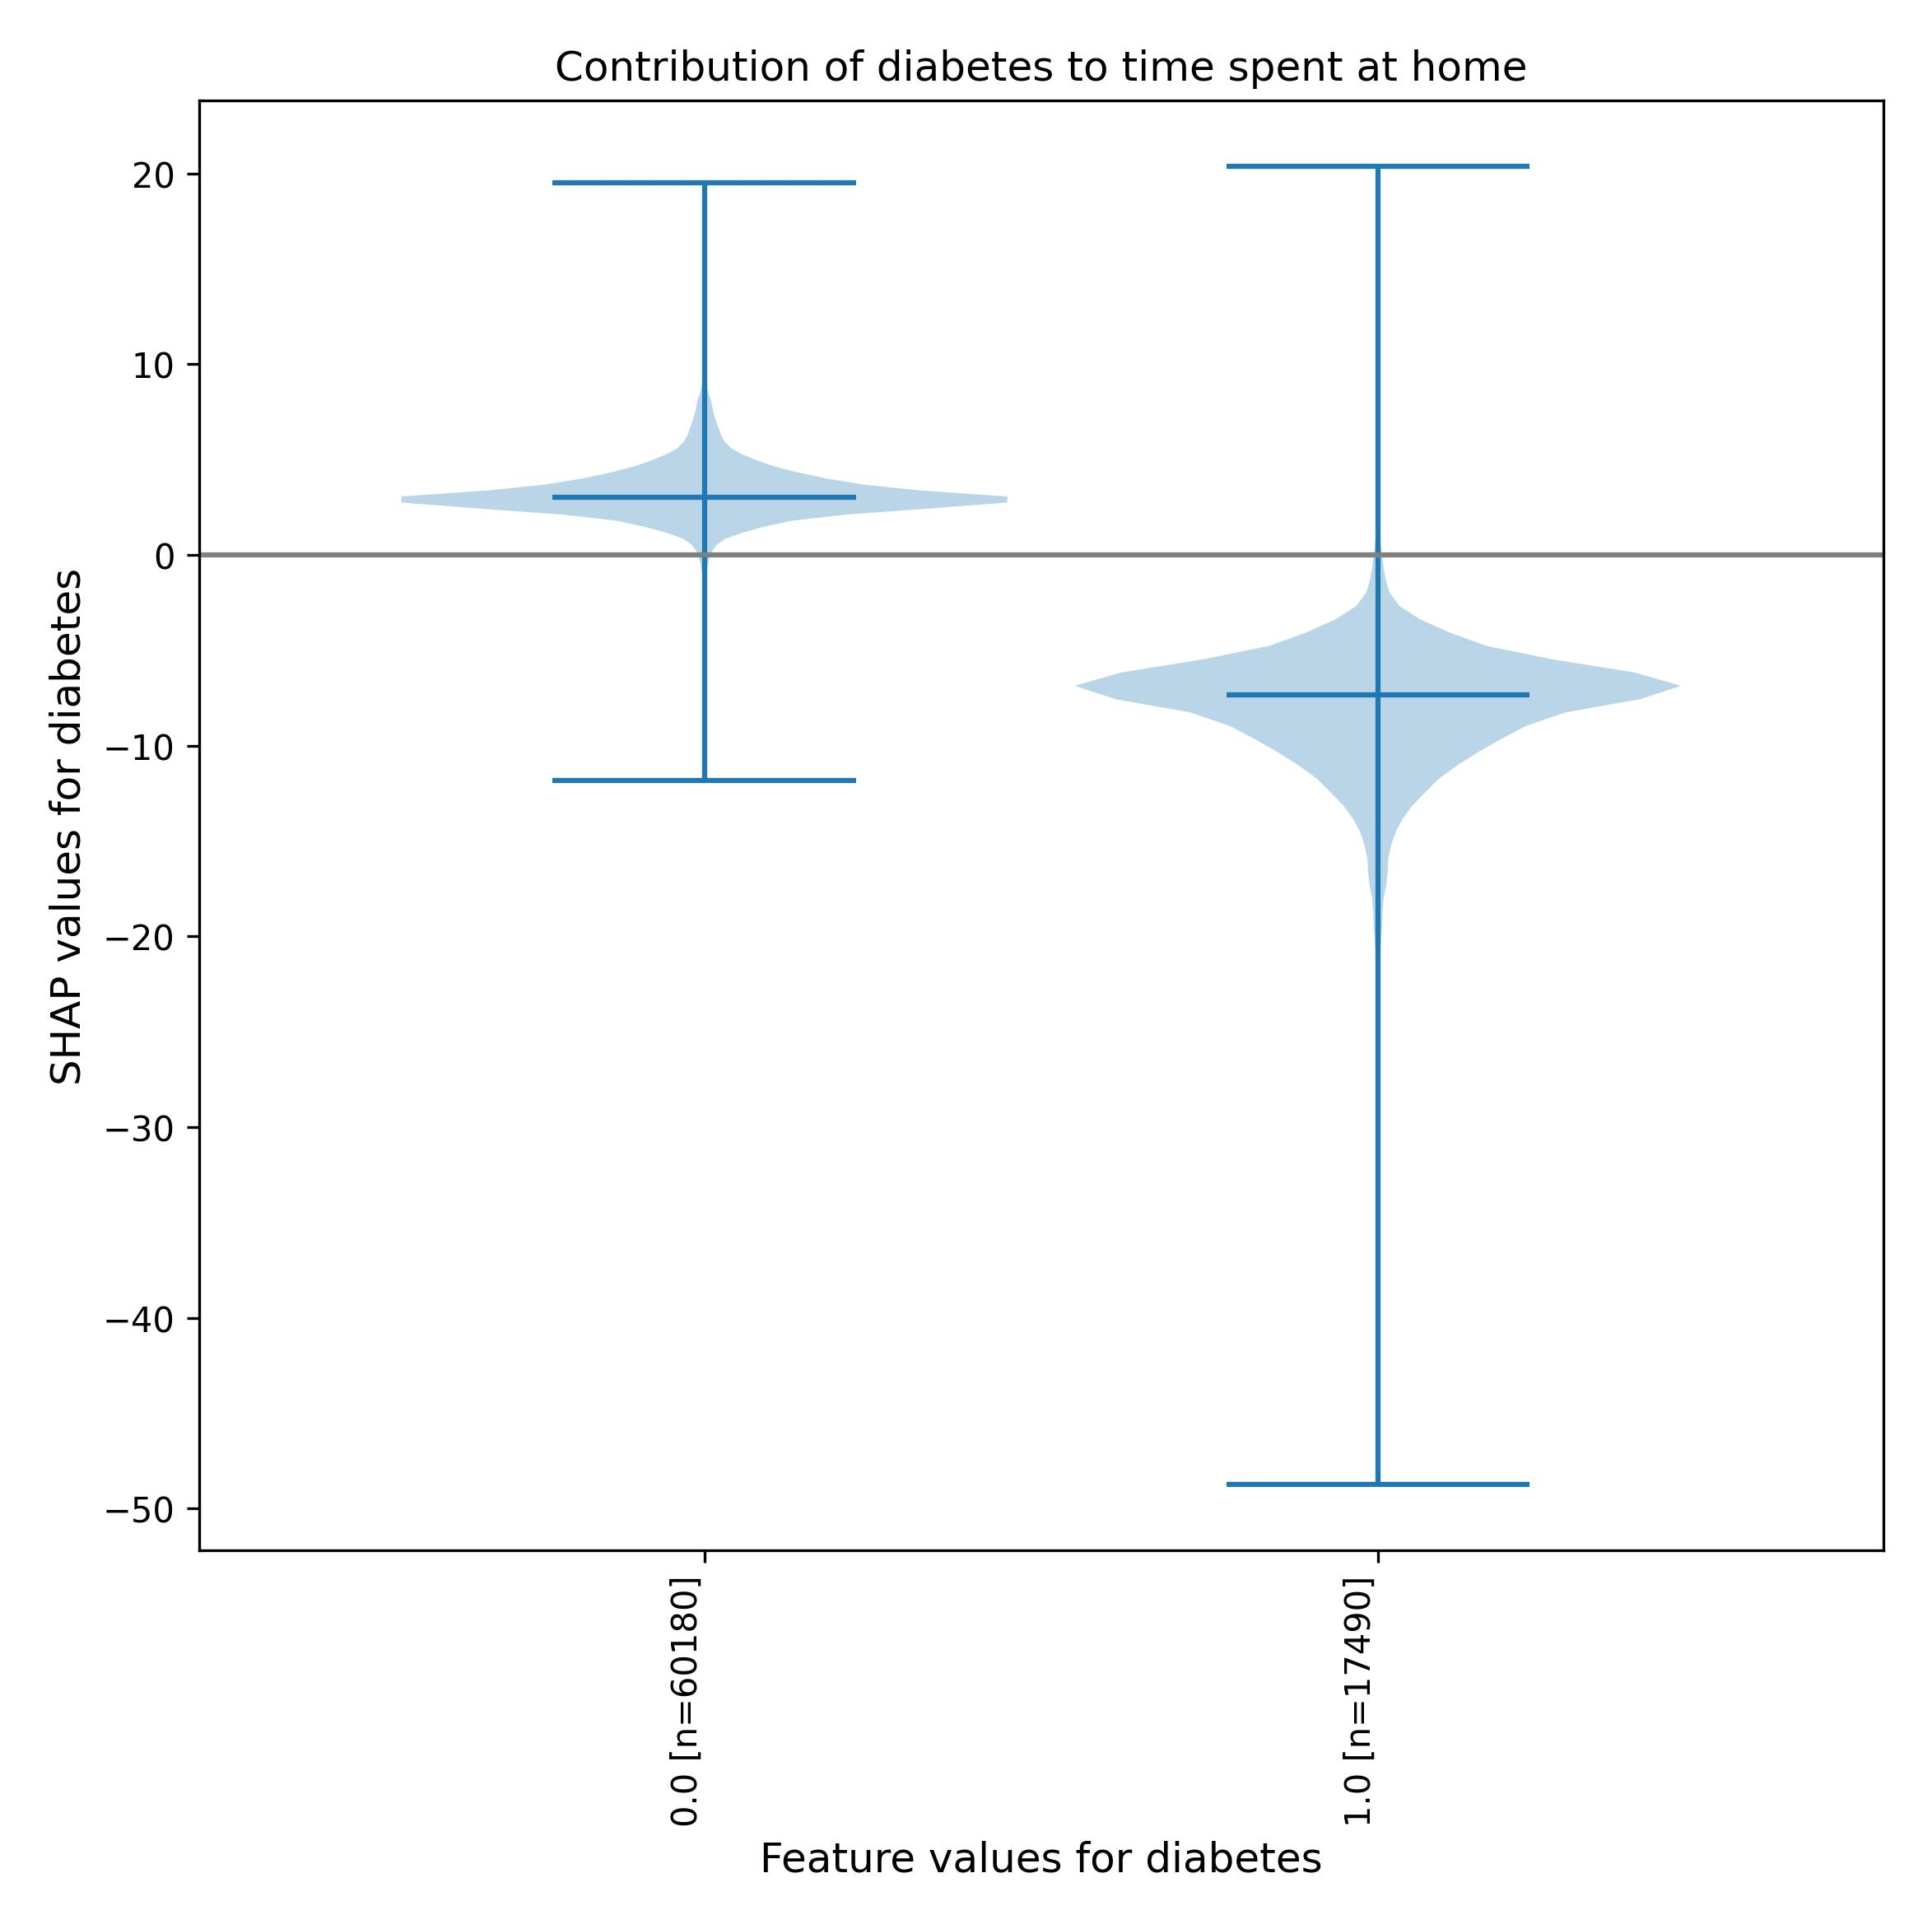
\includegraphics[width=\linewidth]{images/output_results_from_SDE/190_xgboost_at_home_exploratory_population_12_features_violin_shap_diabetes_kfold0.jpg}
        \caption{At home}
        \label{fig:sub8}
    \end{subfigure}
    \hfill
    \begin{subfigure}[t]{0.31\textwidth}
        \centering
        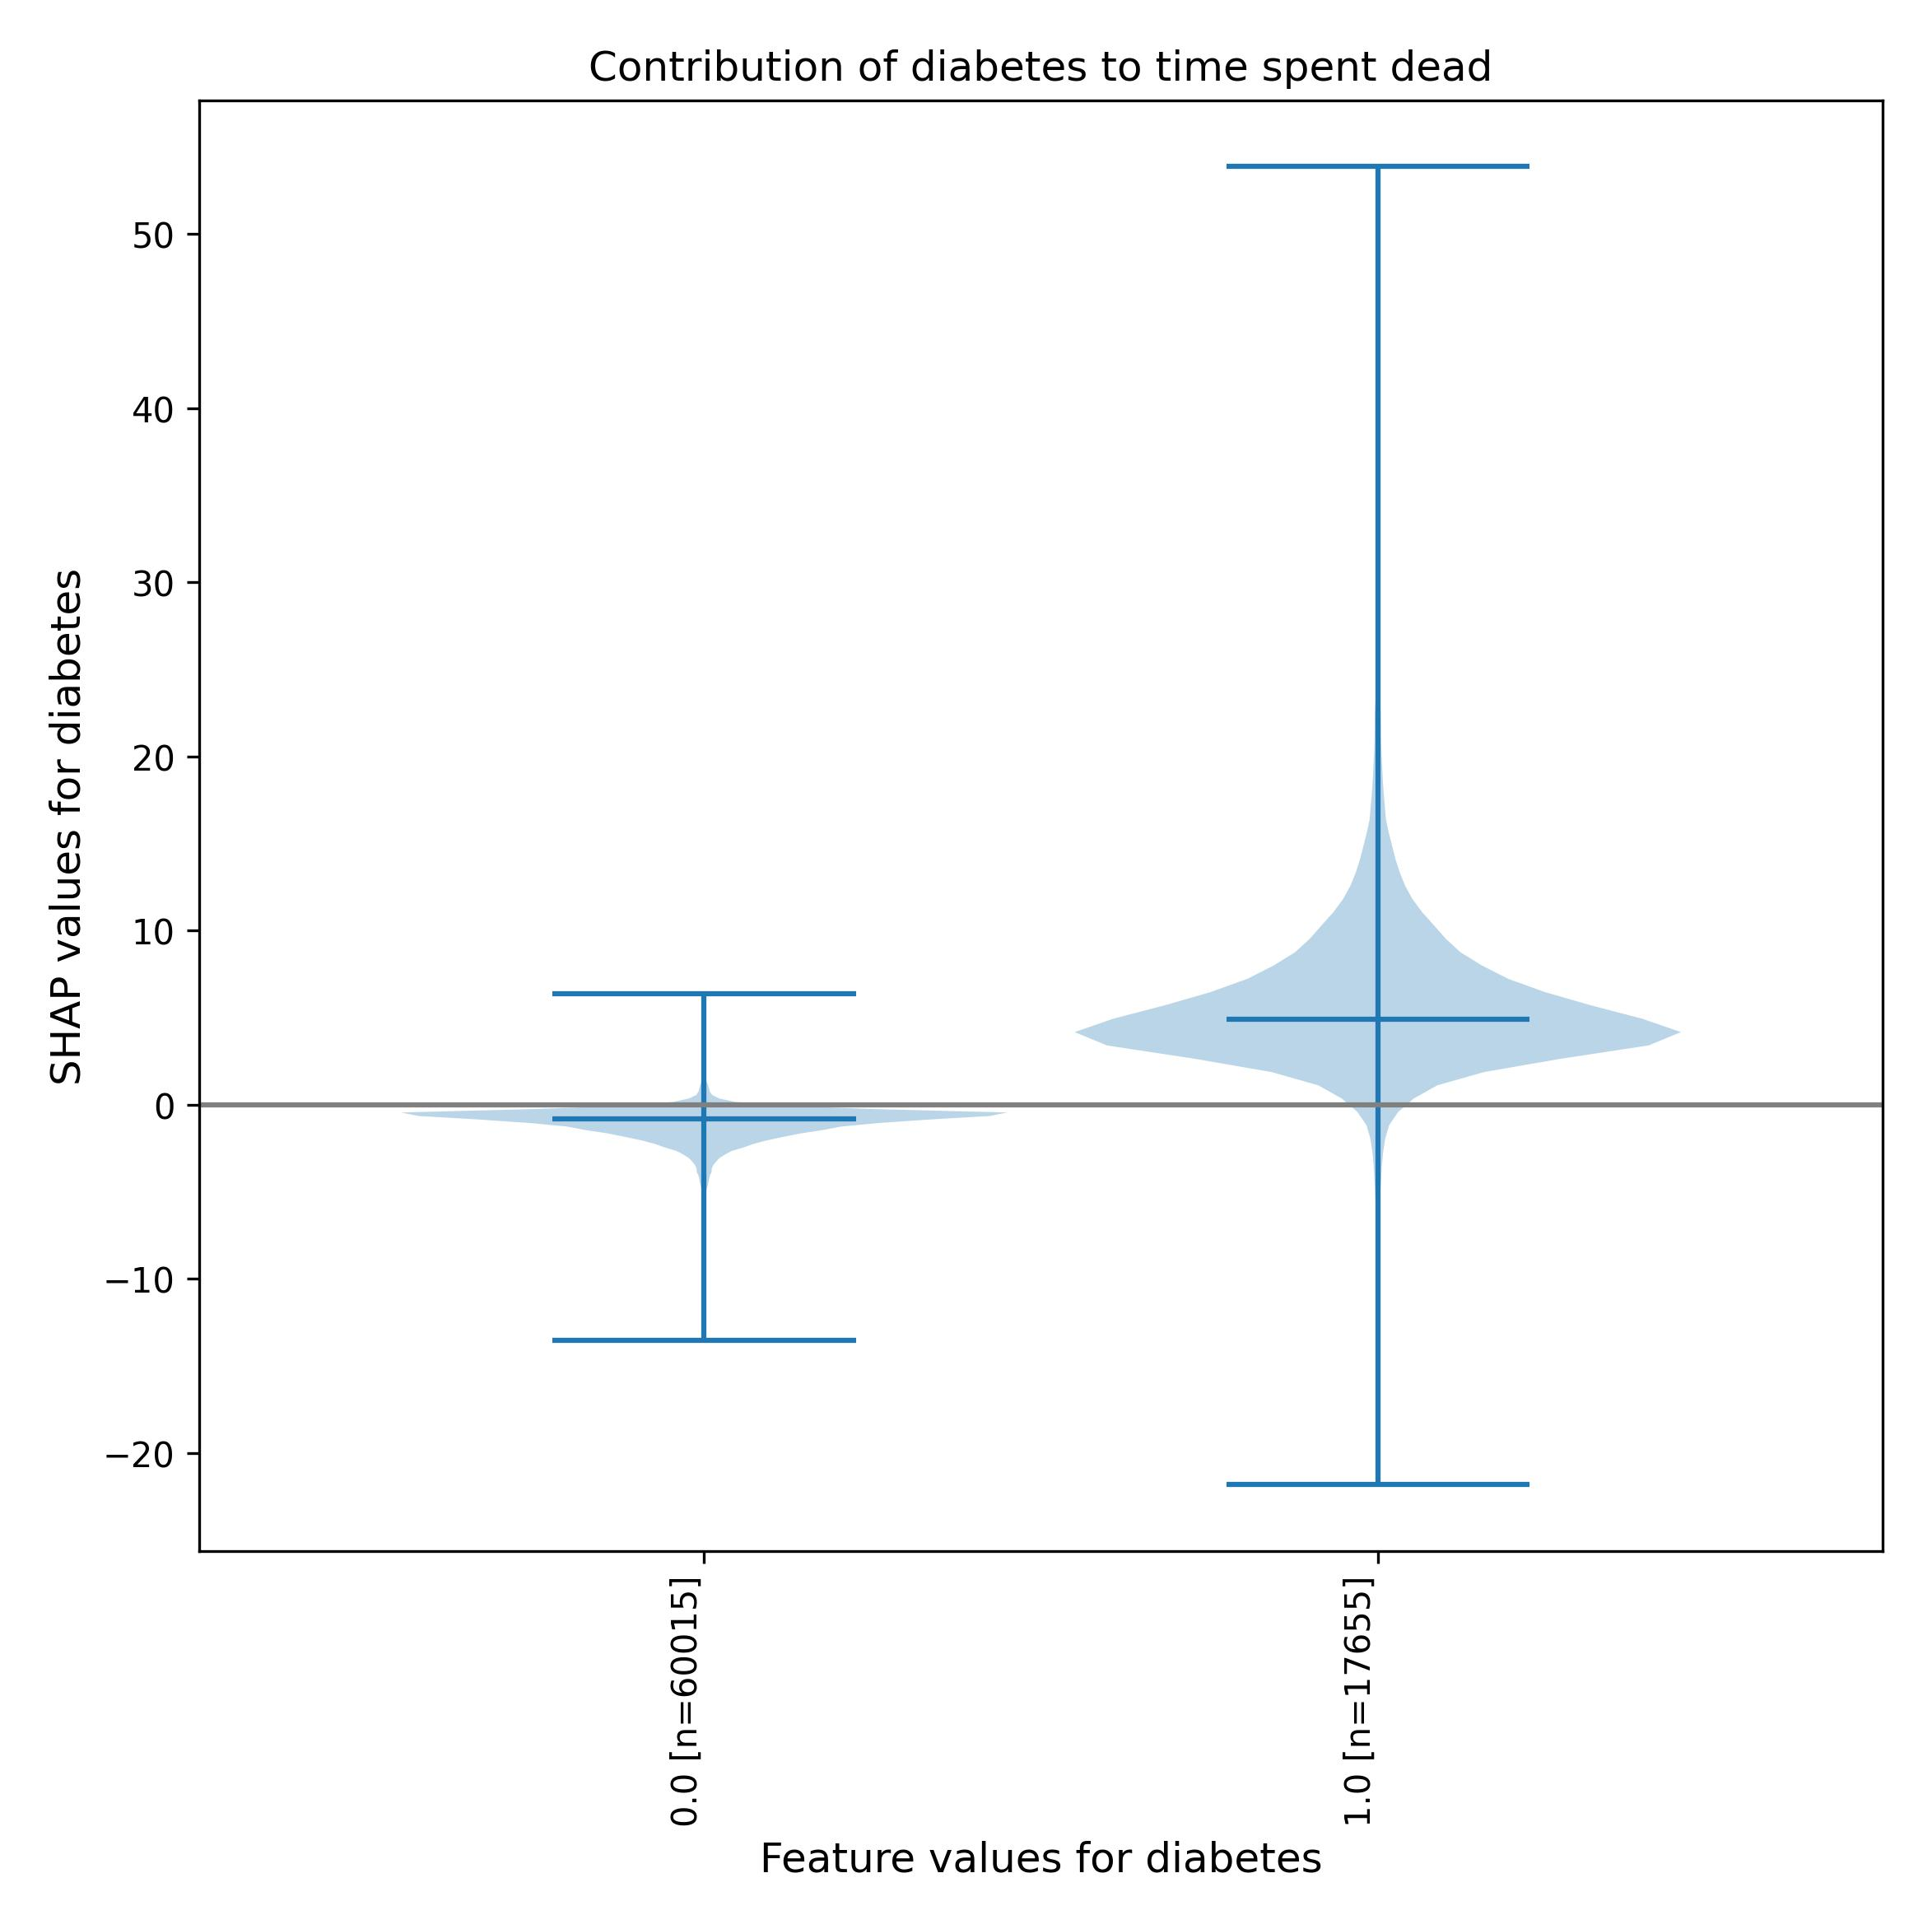
\includegraphics[width=\linewidth]{images/output_results_from_SDE/200_xgboost_dead_exploratory_population_12_features_violin_shap_diabetes_kfold0.jpg}
        \caption{Dead}
        \label{fig:sub9}
    \end{subfigure}
    \caption*{Diabetes}

    \vspace{2em}

    \caption{SHAP analysis on how feature values influence XGBoost model predictions for time spent in a) NHS inpatient care (left), b) at home (alive, and outside of NHS inpatient care), and c) dead, in the year after stroke. Features shown are stroke type (top), diagnosis of atrial fibrillation (middle), and diagnosis of diabetes (bottom). SHAP values are calculated for each prediction, taking into account interactions with other features. The resulting distributions for any given feature value are shown in the figure as violin plots with median and range bars.}
    \label{fig:shap_3}
\end{figure}

%%%%%%%%%%%%%%%%%%%%%%%%%%%%%%%%%%%%%%%%%%%%%%%%%%%%%%%%%%%%%%%%%%%%

\begin{figure}[htbp]
    \centering

    % ---------- Row 1 ----------
    
    \begin{subfigure}[t]{0.31\textwidth}
        \centering
        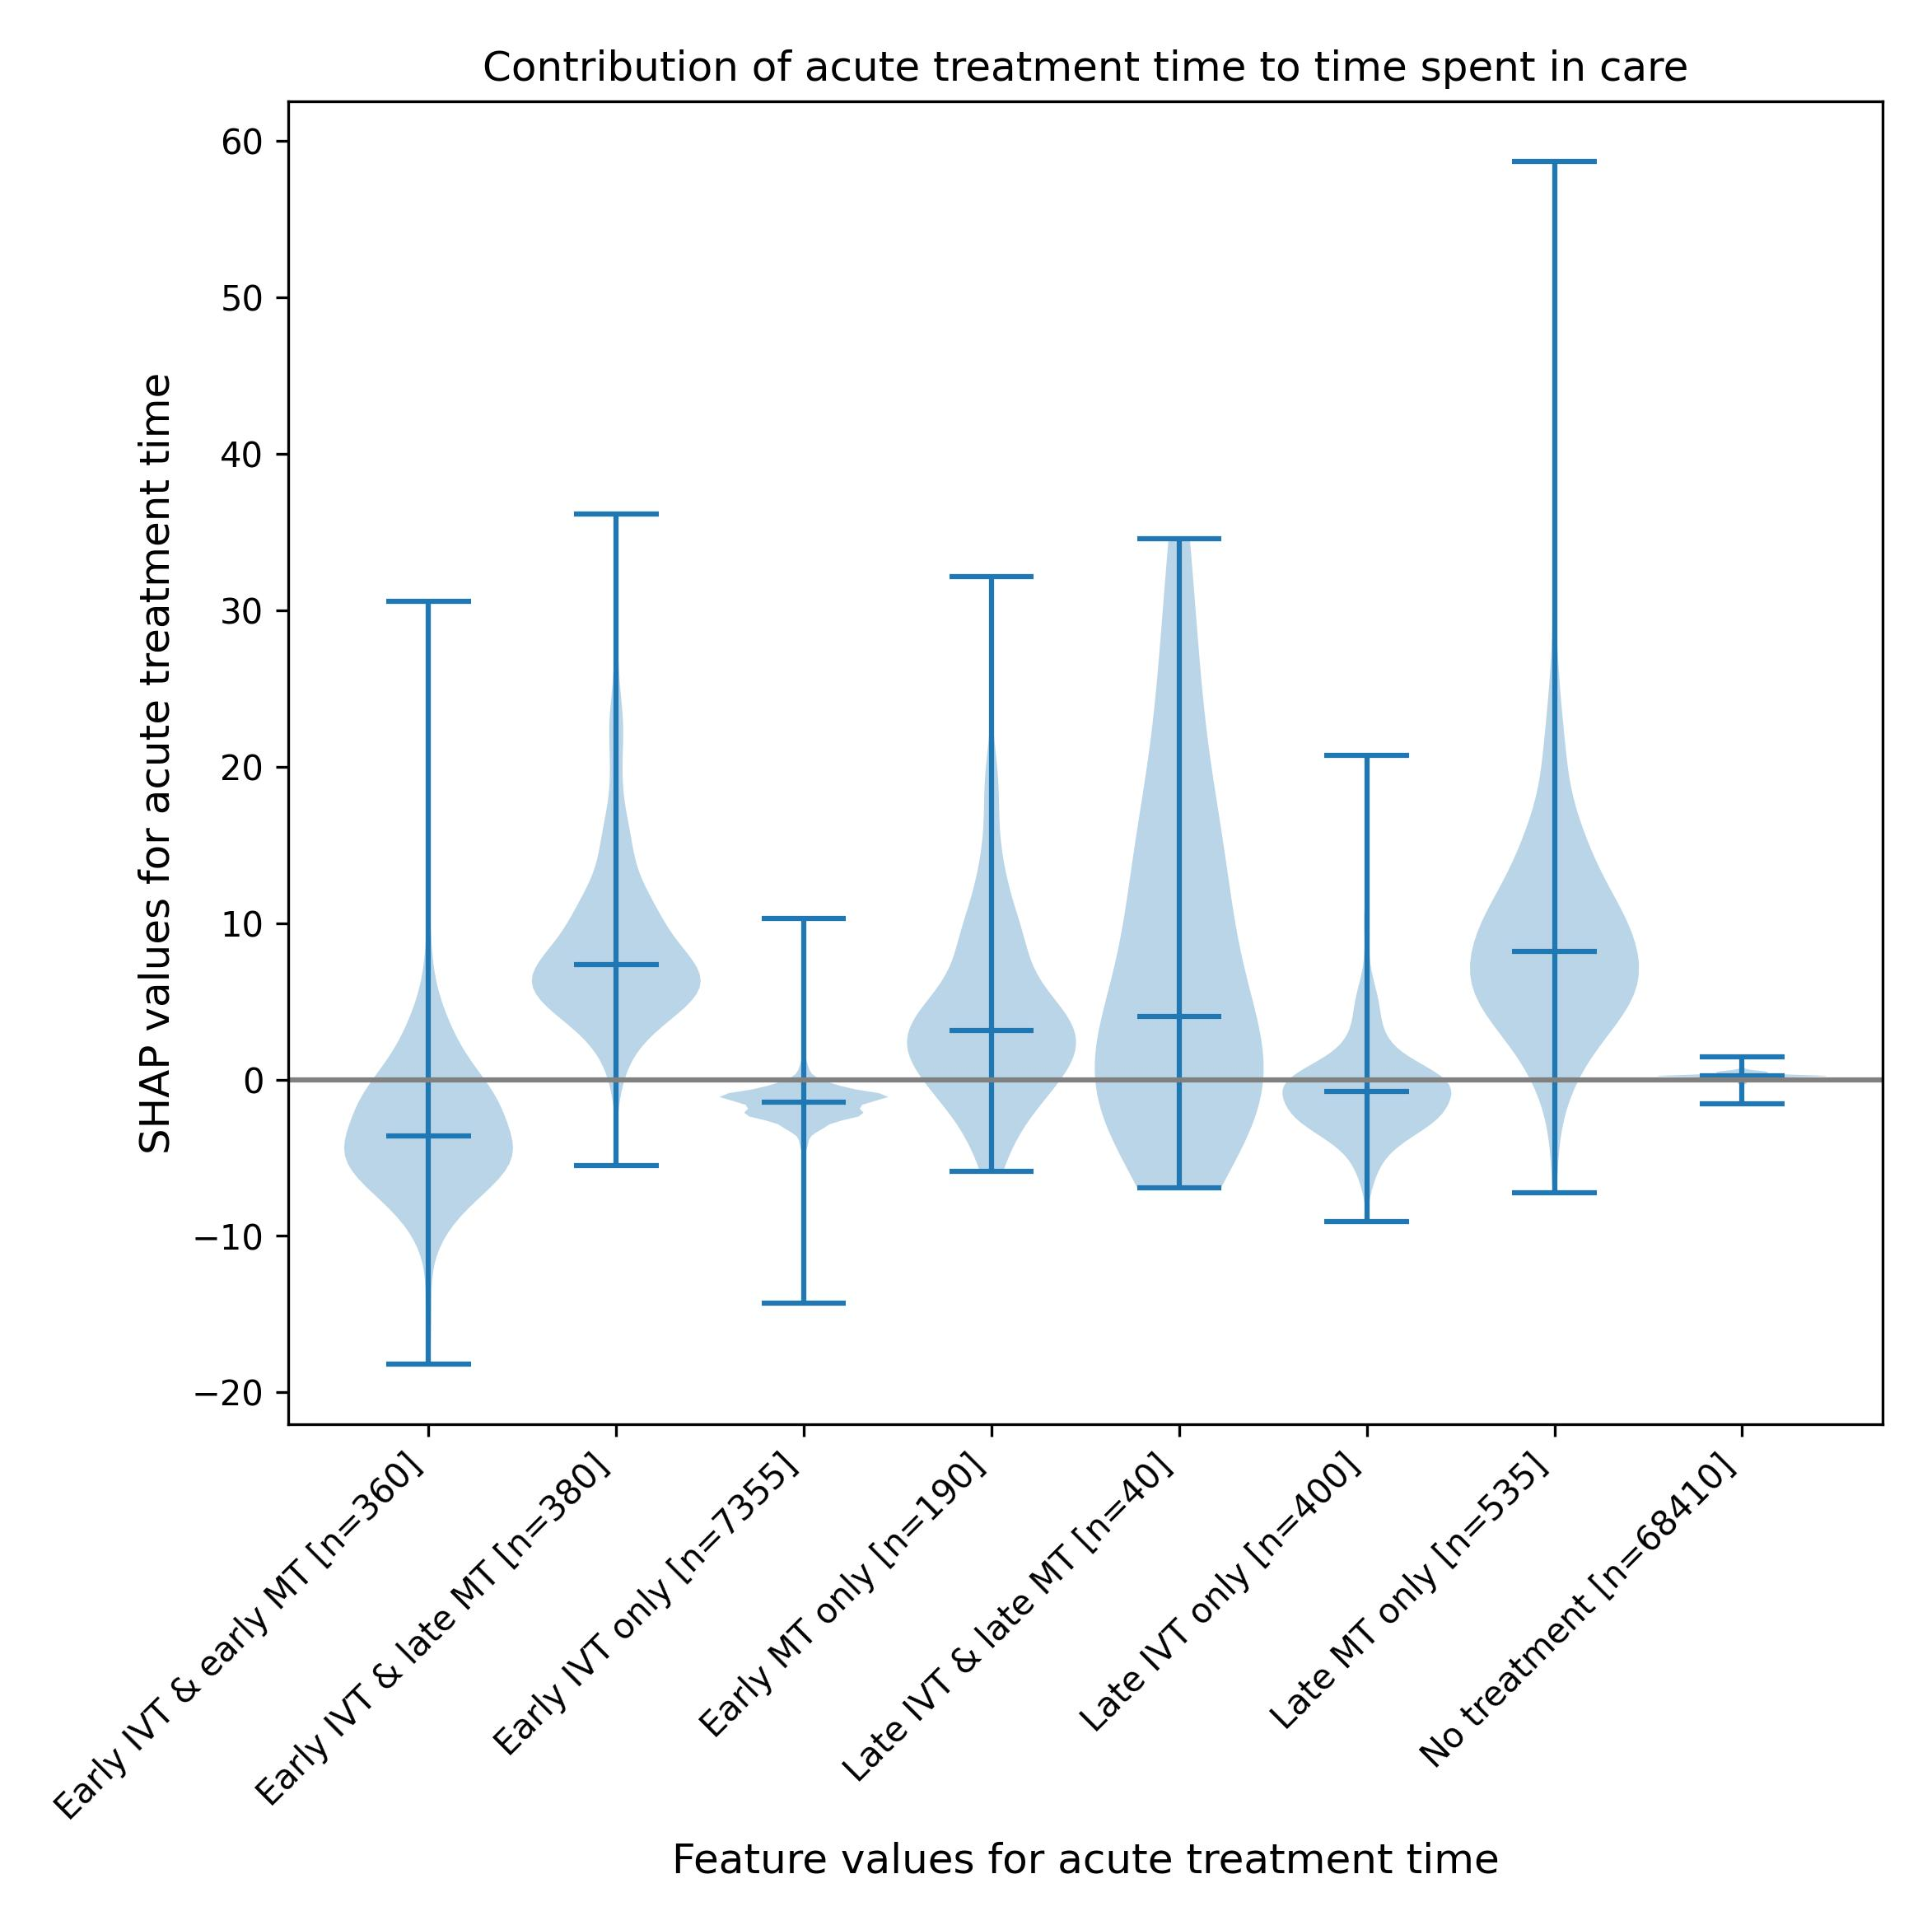
\includegraphics[width=\linewidth]{images/output_results_from_SDE/180_xgboost_in_care_exploratory_population_12_features_shap_violin_acute treatment time_kfold0.jpg}
        \caption{In care}
        \label{fig:sub1}
    \end{subfigure}
    \hfill
    \begin{subfigure}[t]{0.31\textwidth}
        \centering
        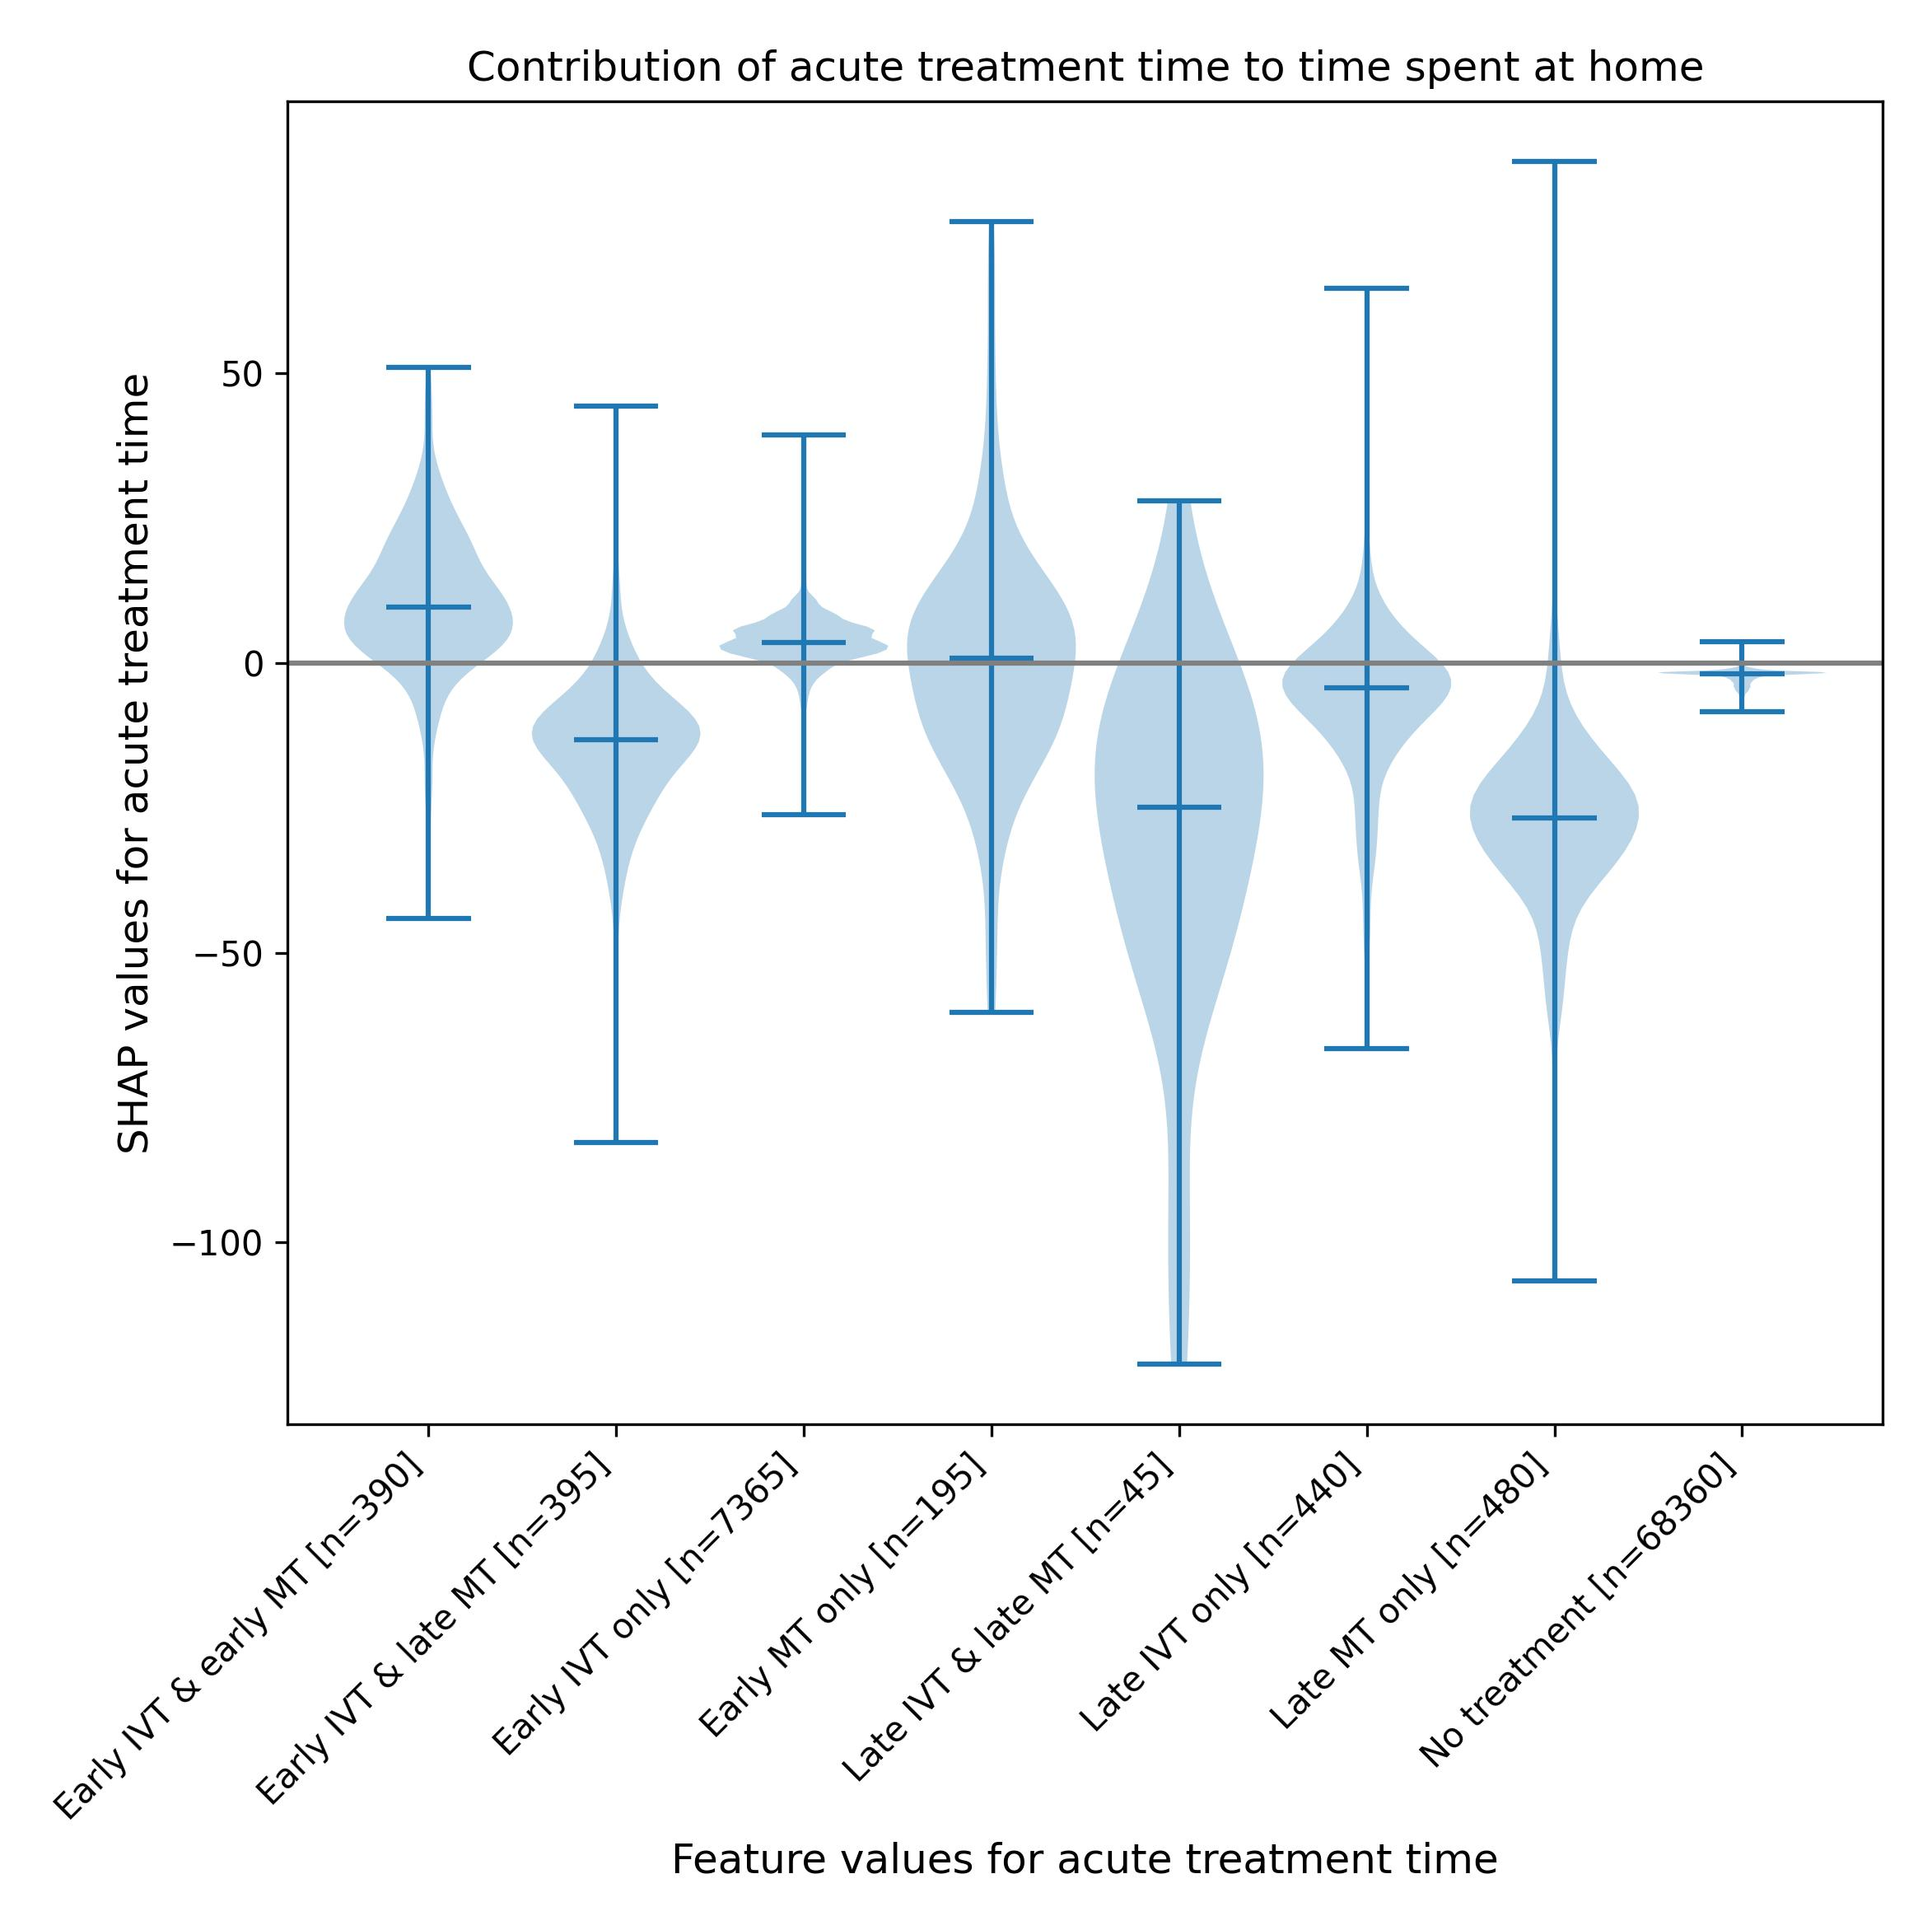
\includegraphics[width=\linewidth]{images/output_results_from_SDE/190_xgboost_at_home_exploratory_population_12_features_shap_violin_acute treatment time_kfold0.jpg}
        \caption{At home}
        \label{fig:sub2}
    \end{subfigure}
    \hfill
    \begin{subfigure}[t]{0.31\textwidth}
        \centering
        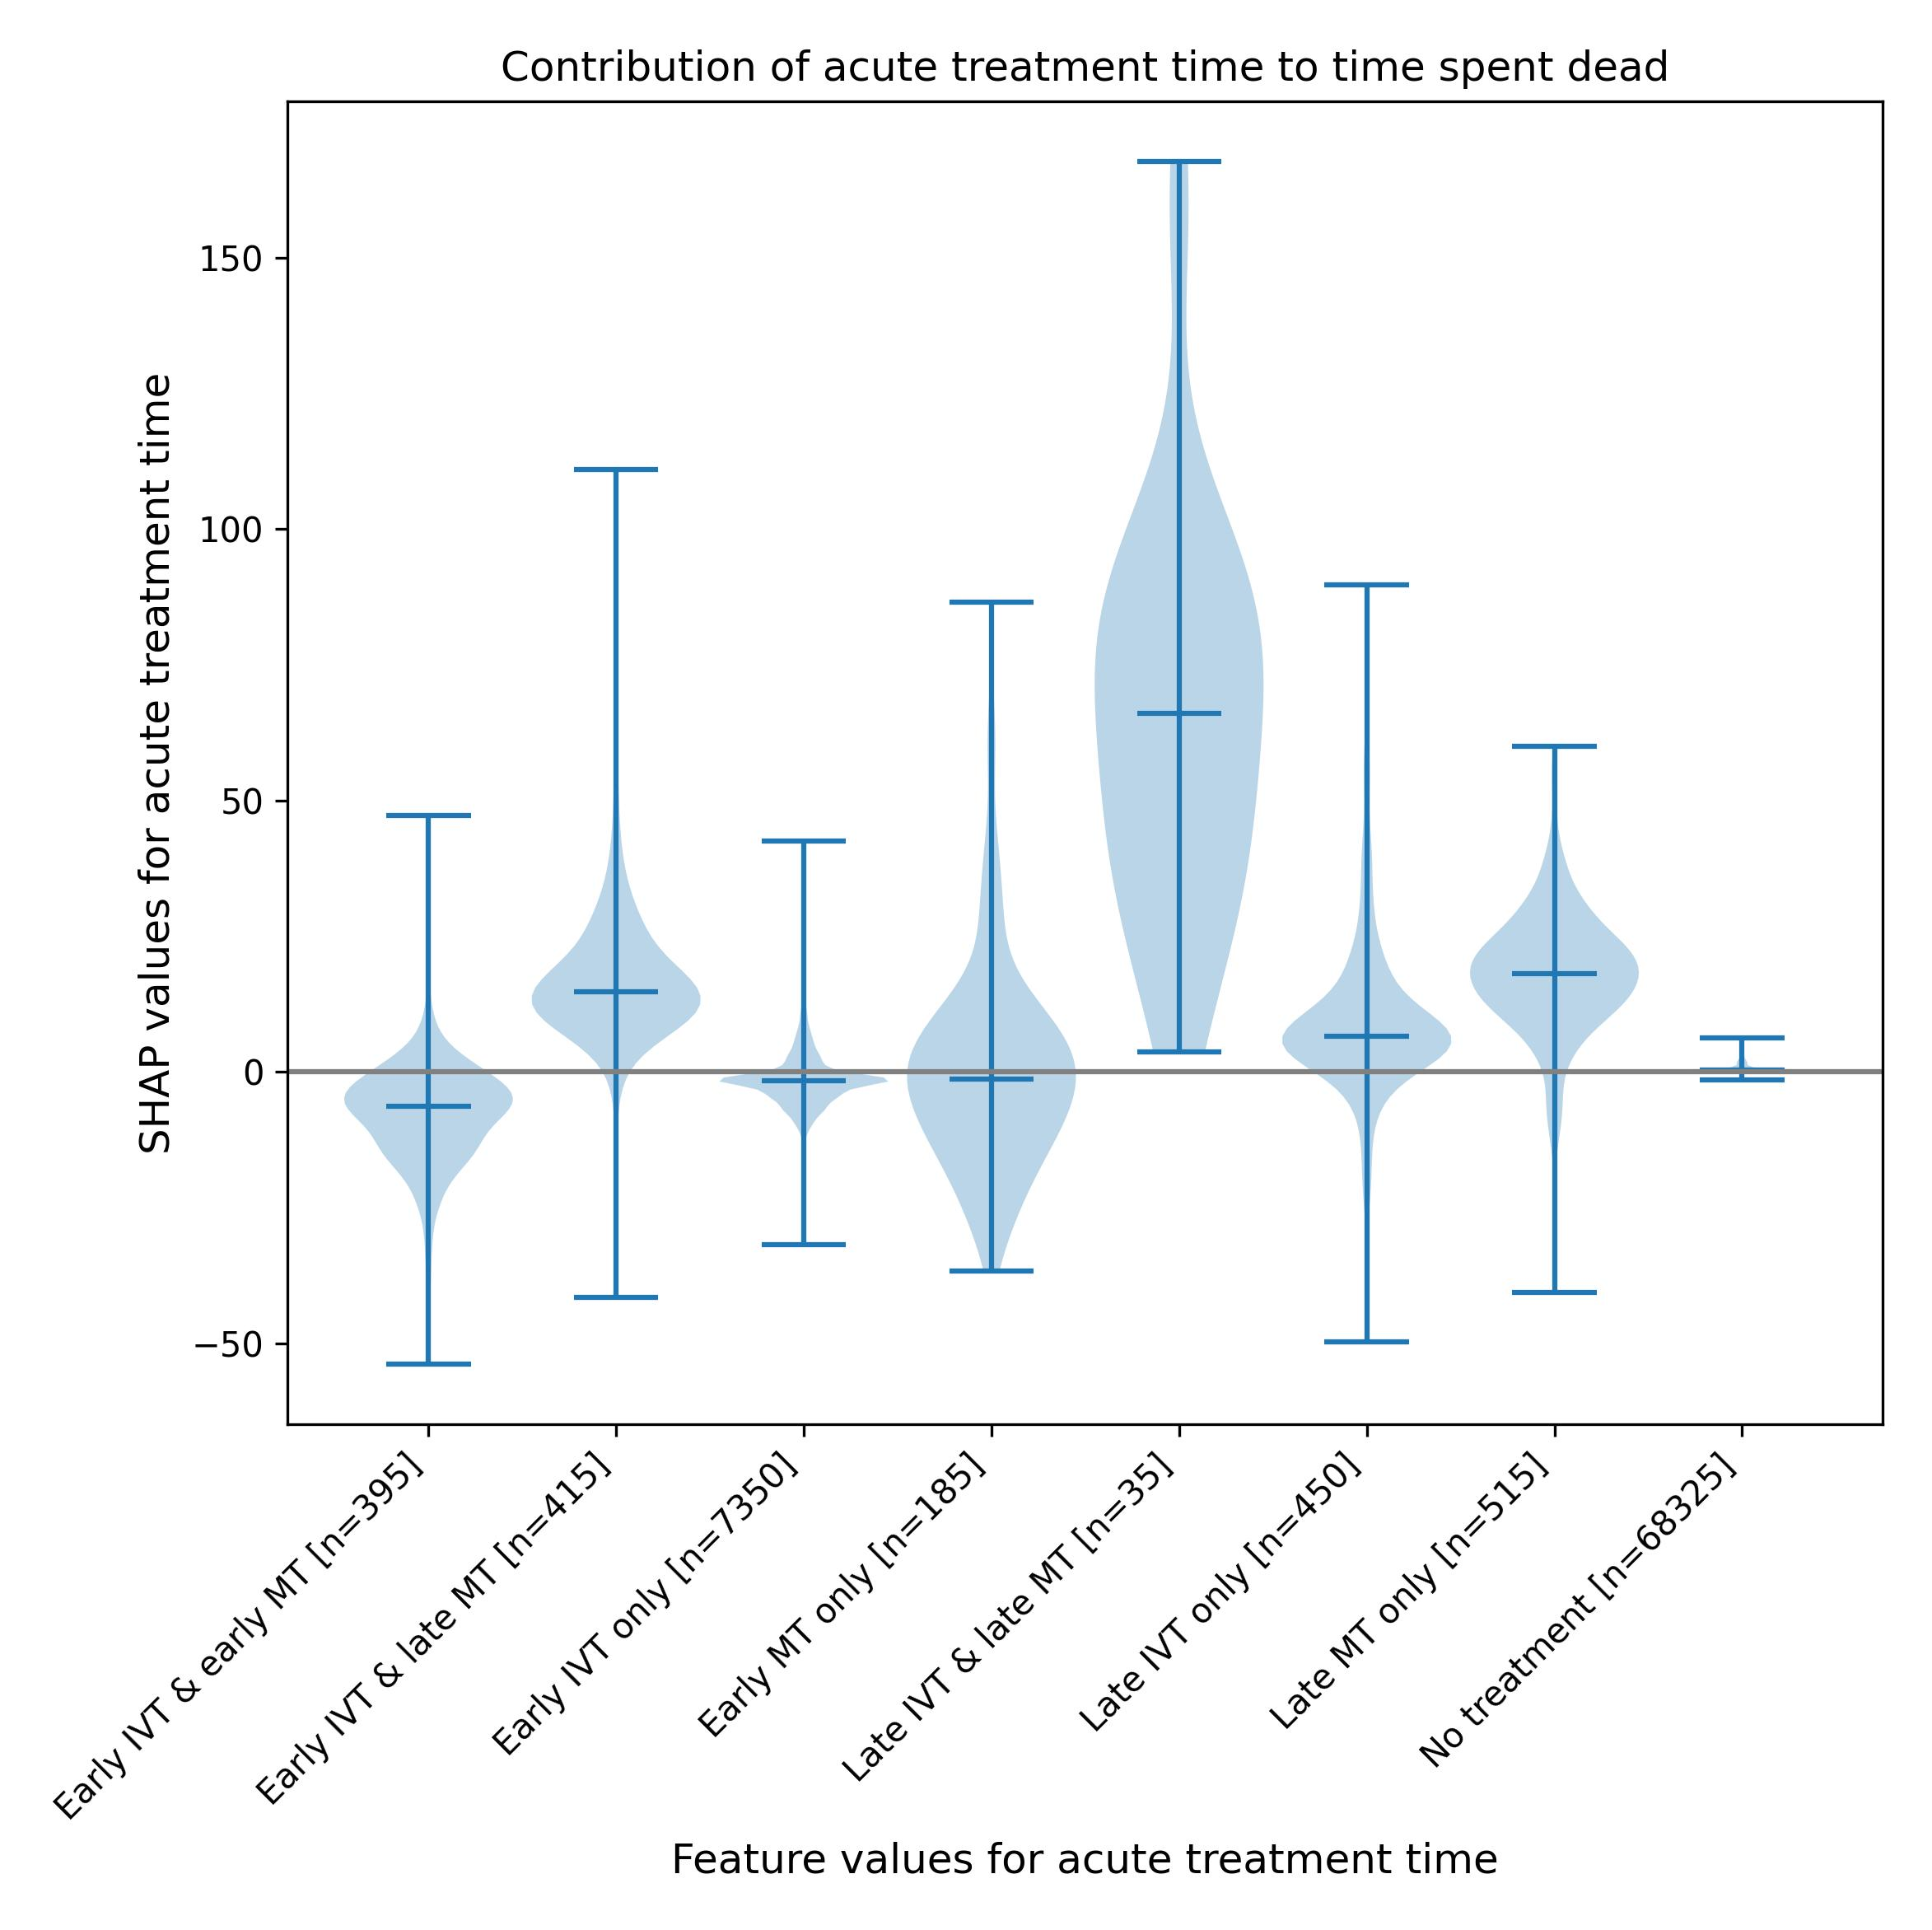
\includegraphics[width=\linewidth]{images/output_results_from_SDE/200_xgboost_dead_exploratory_population_12_features_shap_violin_acute treatment time_kfold0.jpg}
        \caption{Dead}
        \label{fig:sub3}
    \end{subfigure}
    \caption*{Treatment (full population and model)}

    \vspace{2em} % space between rows

        \begin{subfigure}[t]{0.31\textwidth}
        \centering
        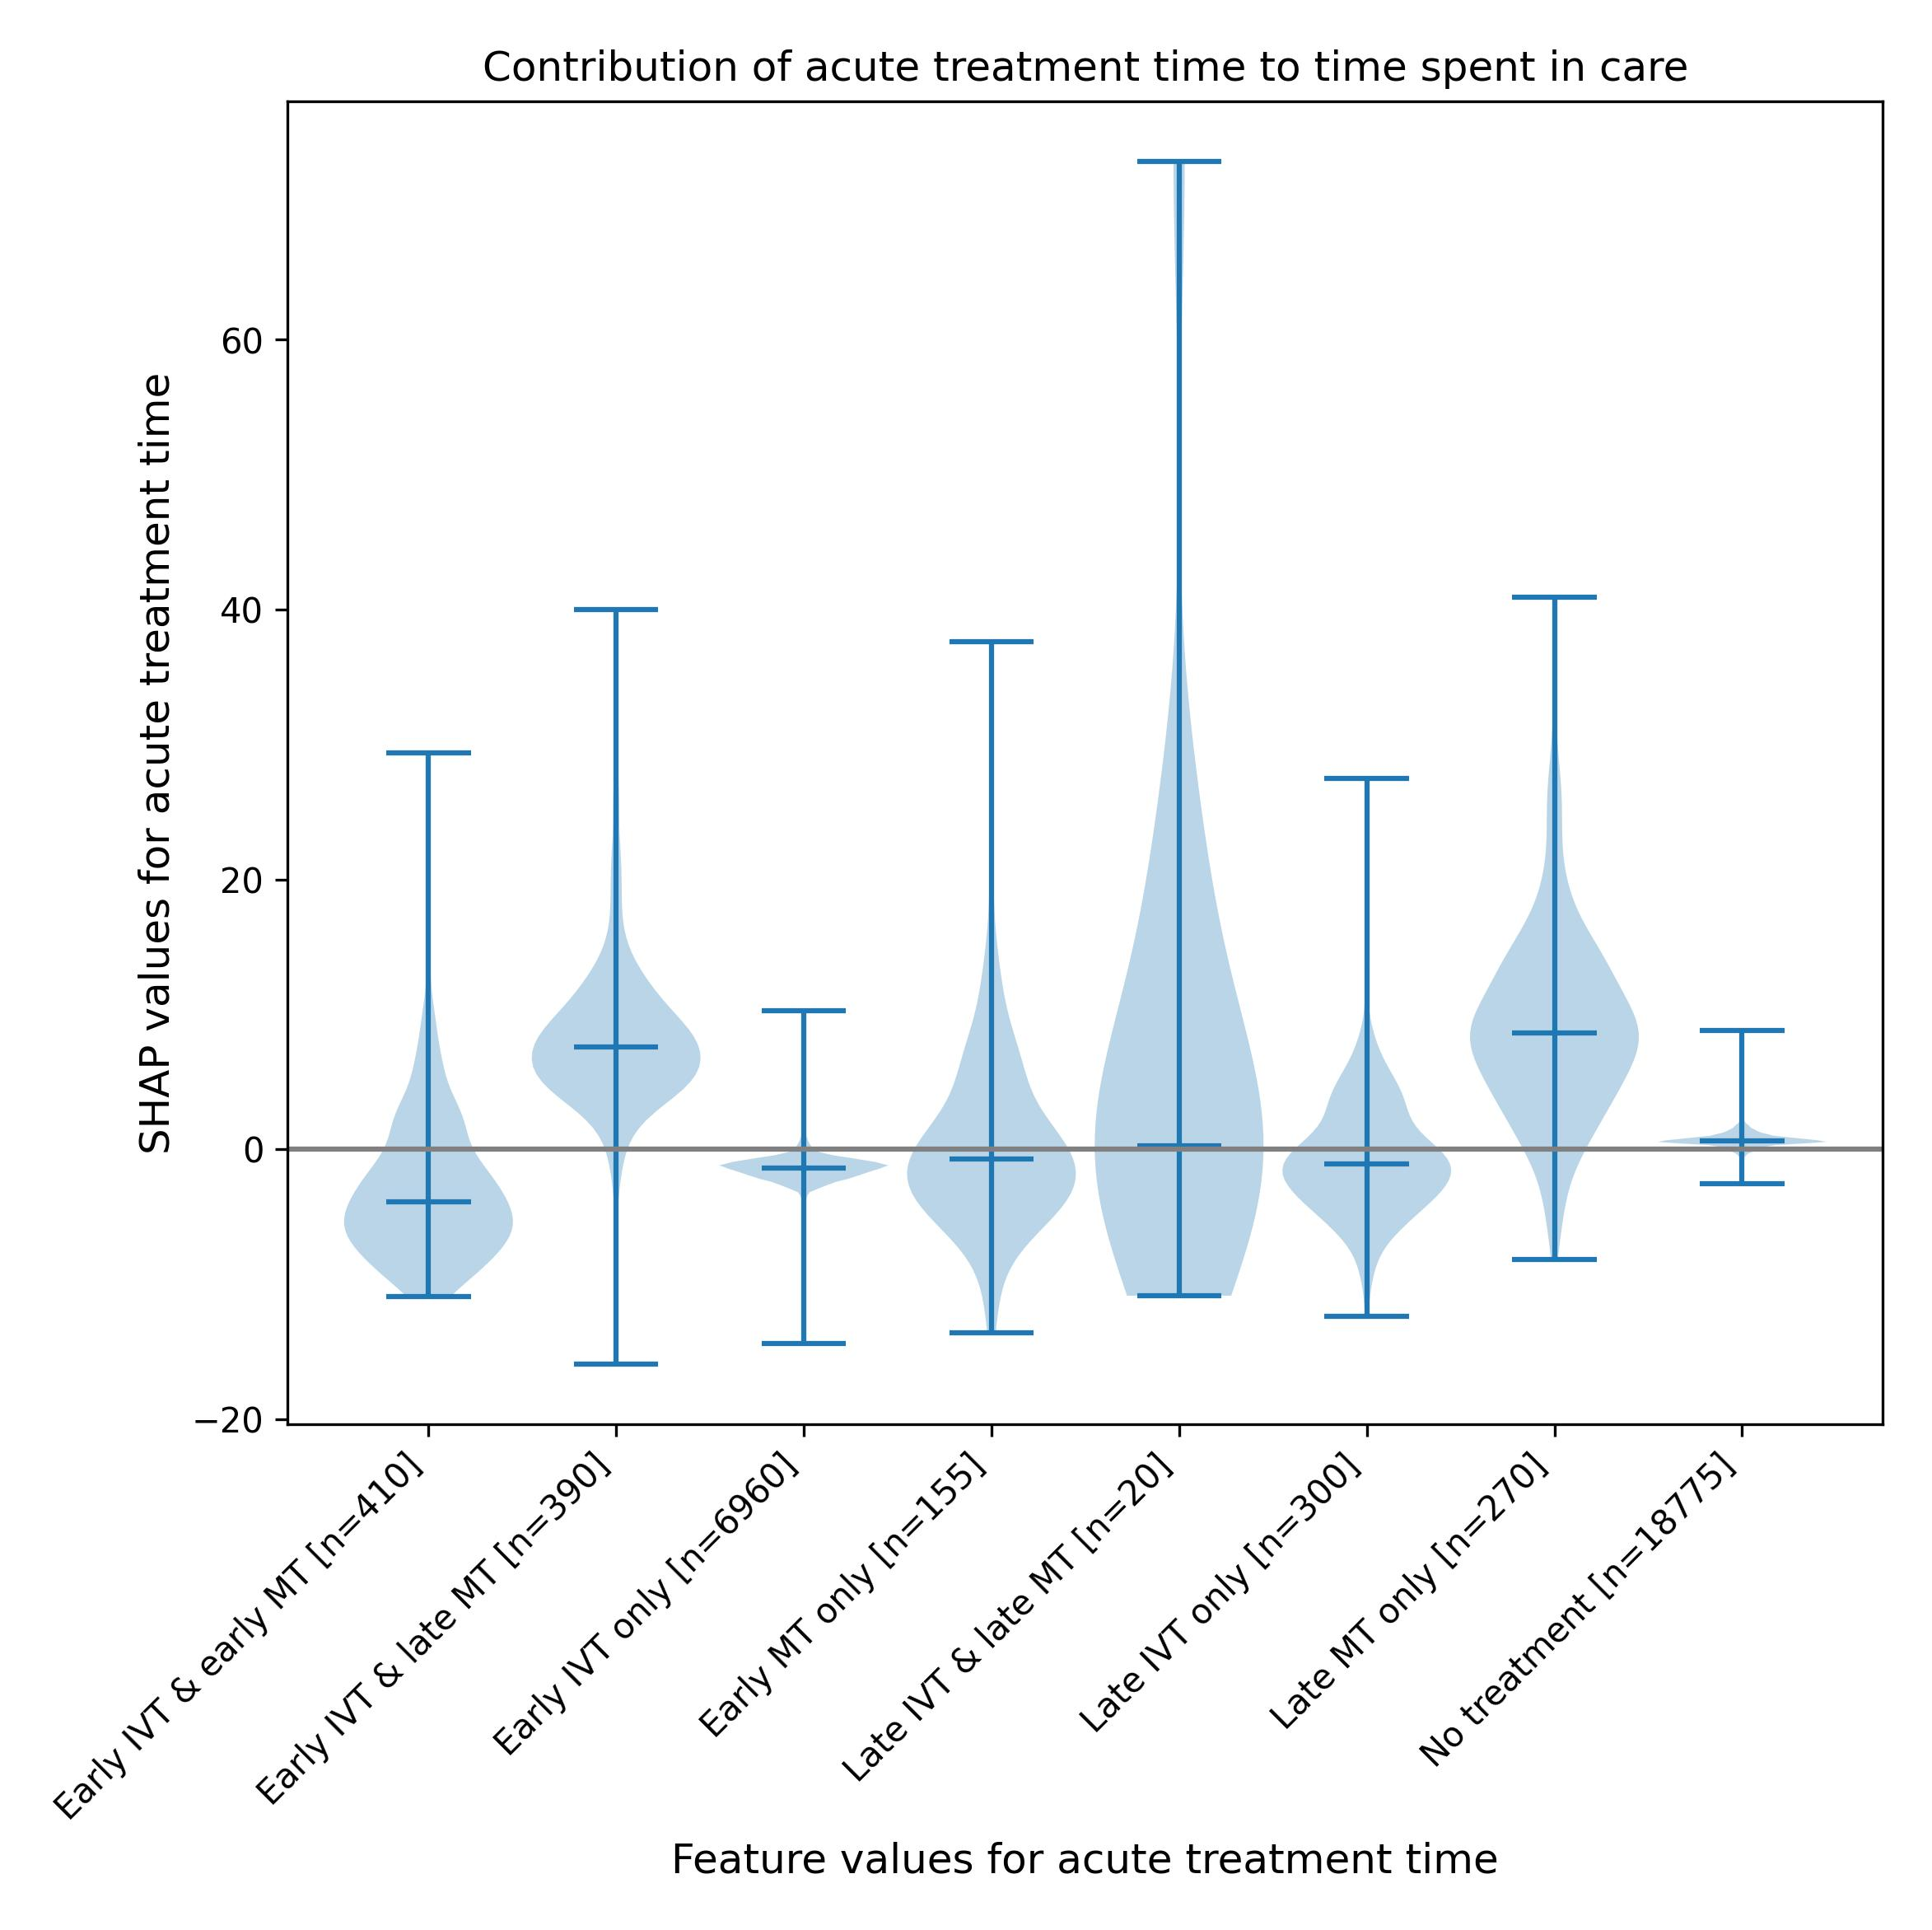
\includegraphics[width=\linewidth]{images/output_results_from_SDE/210_xgboost_in_care_causal_population_6_features_shap_violin_acute treatment time_kfold0}
        \caption{In care}
        \label{fig:sub1}
    \end{subfigure}
    \hfill
    \begin{subfigure}[t]{0.31\textwidth}
        \centering
        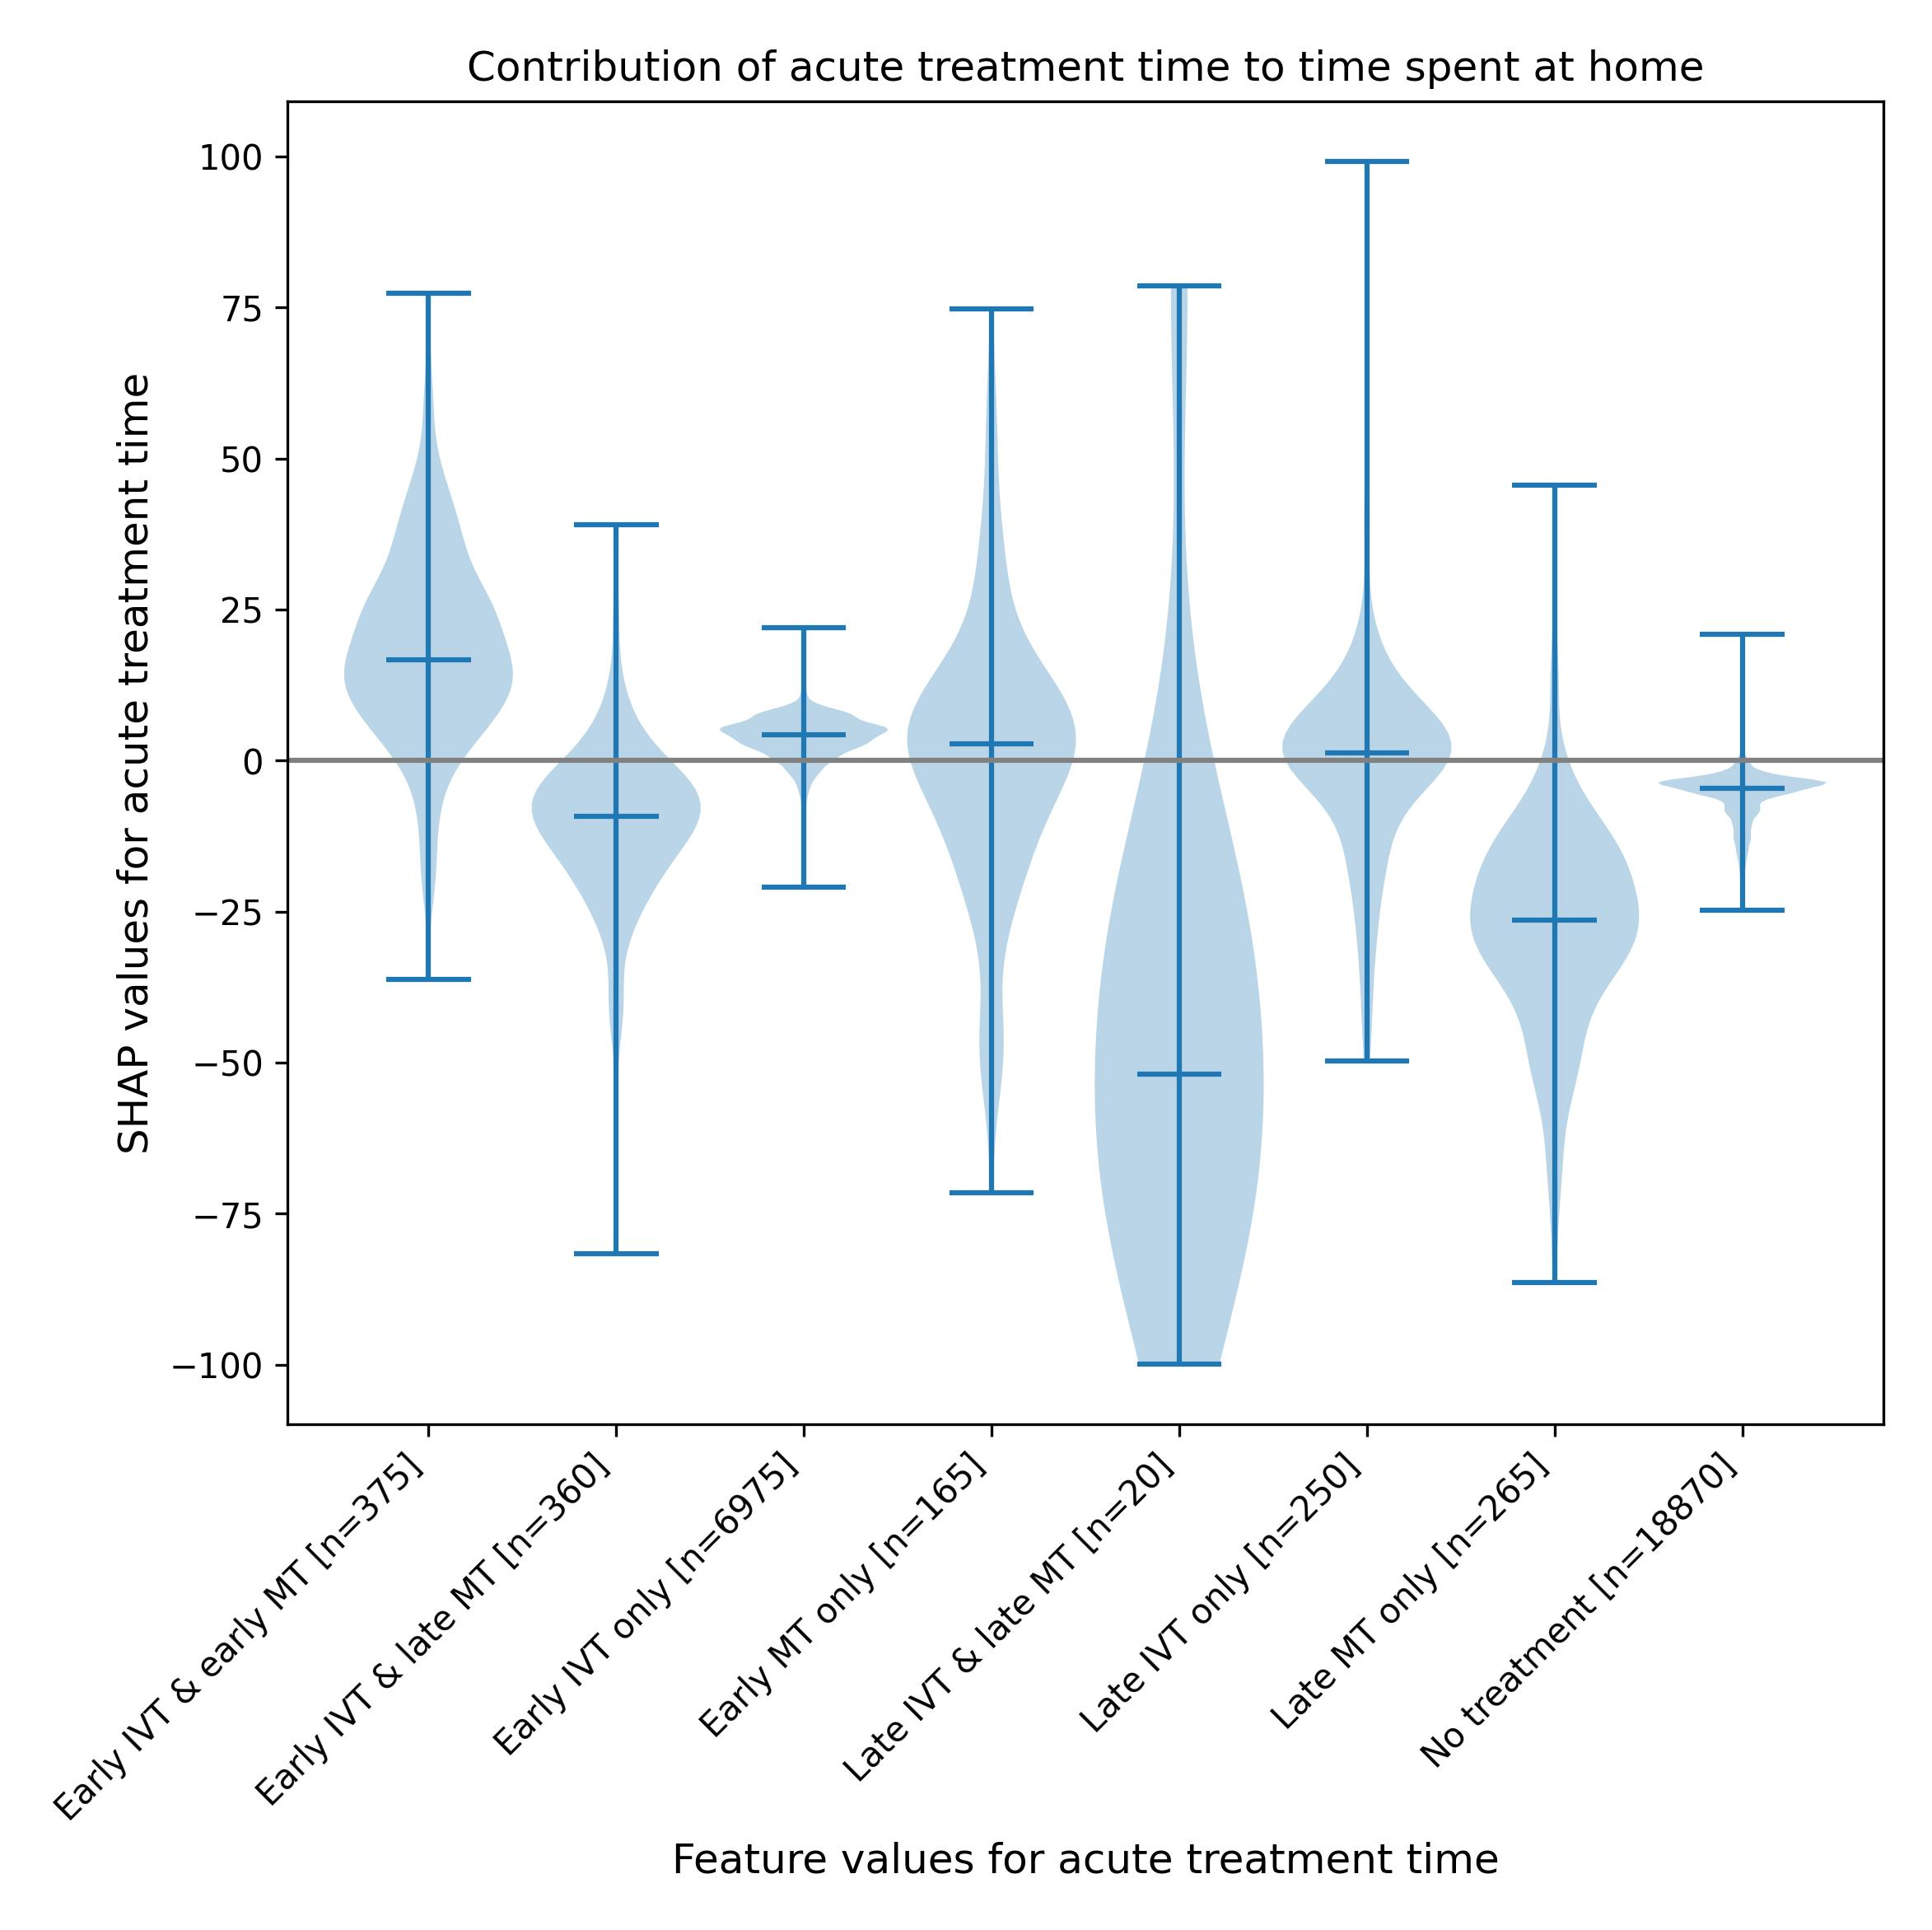
\includegraphics[width=\linewidth]{images/output_results_from_SDE/220_xgboost_at_home_causal_population_6_features_shap_violin_acute treatment time_kfold0}
        \caption{At home}
        \label{fig:sub2}
    \end{subfigure}
    \hfill
    \begin{subfigure}[t]{0.31\textwidth}
        \centering
        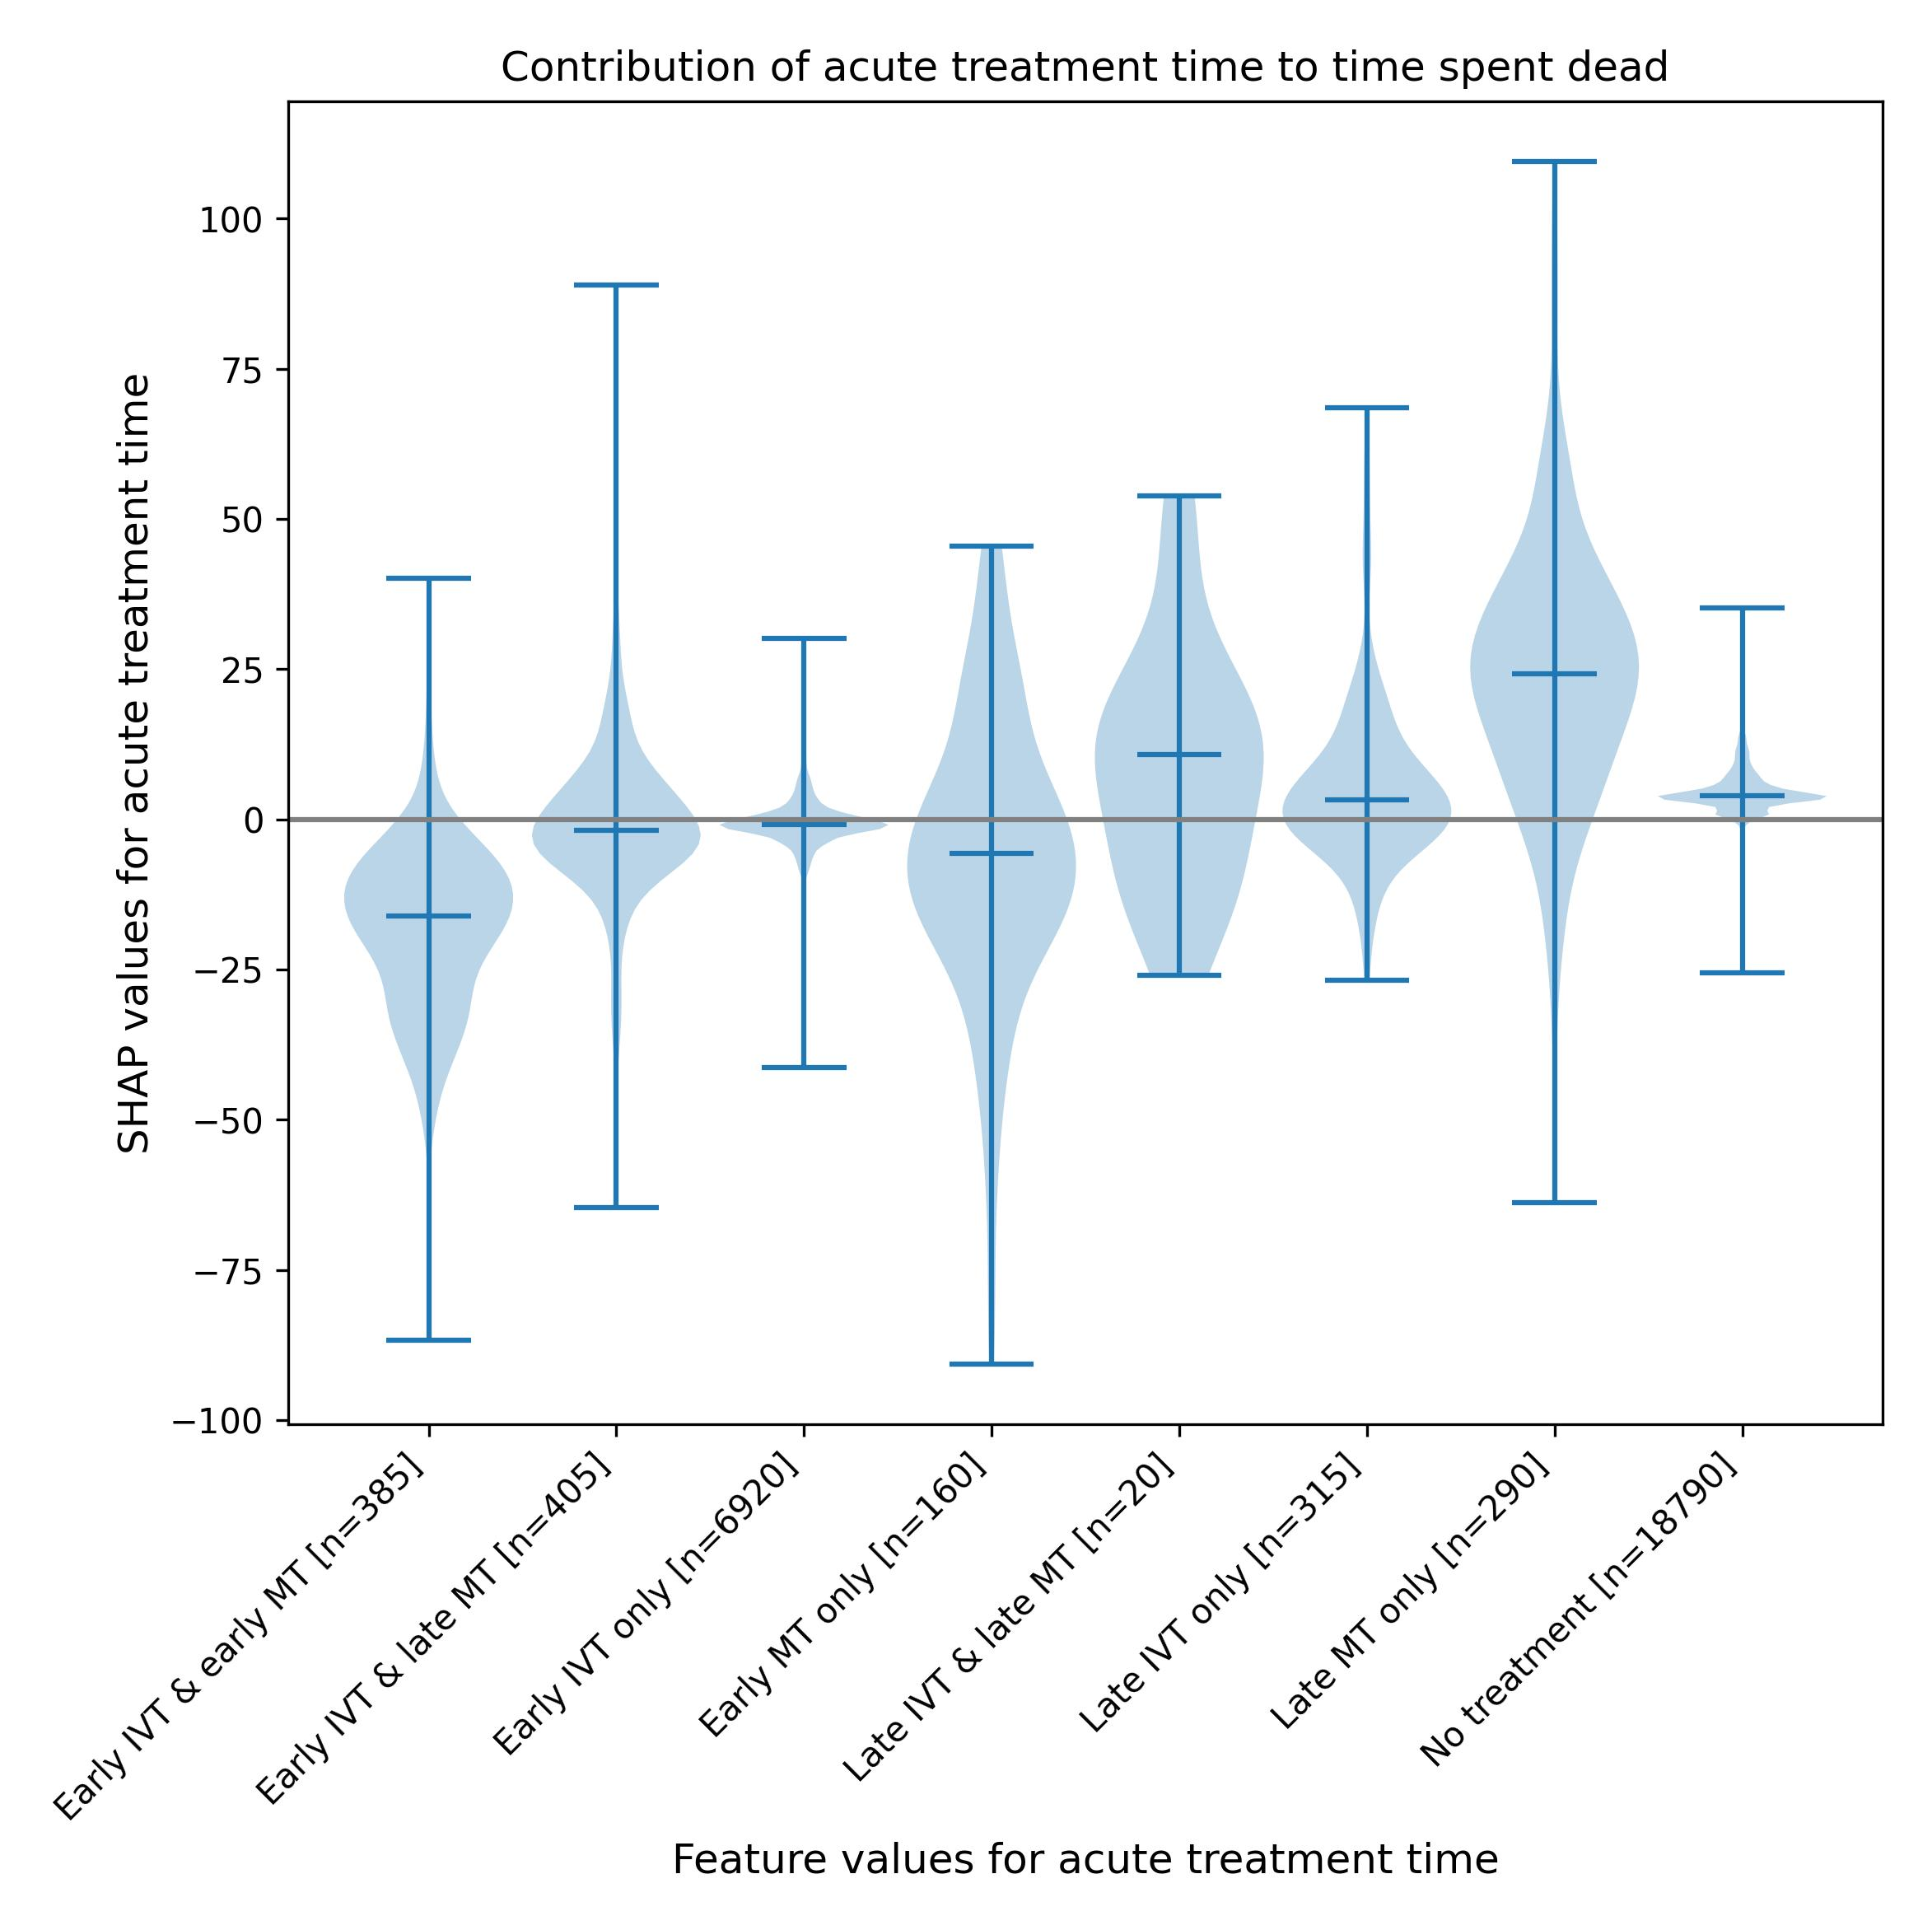
\includegraphics[width=\linewidth]{images/output_results_from_SDE/230_xgboost_dead_causal_population_6_features_shap_violin_acute treatment time_kfold0}
        \caption{Dead}
        \label{fig:sub3}
    \end{subfigure}
    \caption*{Treatment (reperfusion analysis cohort)}


    \vspace{2em}

    \caption{SHAP analysis on how feature values influence XGBoost model predictions for time spent in a) NHS inpatient care (left), b) at home (alive, and outside of NHS inpatient care), and c) dead, in the year after stroke. Features shown are reperfusion treatment received, and time of that treatment (`\textit{early}' defined as before 4.5 hours, and `\textit{late}' as after 4.5 hours, from time of stroke onset). The top panel shows SHAP values in the full stroke population using 12 selected features, and the bottom panel shows SHAP values in the reperfusion treatment cohort with a focused 8 features, designed to strengthen proper isolation of treatment effect. SHAP values are calculated for each prediction, taking into account interactions with other features. The resulting distributions for any given feature value are shown in the figure as violin plots with median and range bars.}
    \label{fig:shap_4}
\end{figure}